\documentclass[twoside,cjk,UTF8]{nputhesis}
\graphicspath{{figure/chapter2/}}
\graphicspath{{figure/chapter5/}}  % 图片文件夹,无需再加,类似于addpath
\begin{document}
\schoolno{10699}
%\classno{}
%\secretlevel{}
\title[ Binaural Rendering Technology In Augmented Reality ]{	增强现实中\\双耳渲染技术研究}
\author[Jieru Chen]{陈洁茹}
\authorno{2018200480}
\major[Signal and Information Processing]{信号与信息处理}
\supervisor[Wen~Zhang~,~Jingdong~Chen]{张雯~~陈景东}
\applydate[March 2021]{2021~年~3~月}
\support{本文研究得到XX基金(编号:XXXXXXX)资助。}
\makecover

\frontmatter
% 中文摘要
\support{本文研究得到XX基金(编号:XXXXXXX)资助。}
\begin{abstract}
	
这是一段摘要

	%\lipsum[2-3]
	\begin{keywords}
		关键词、关键词、关键词
	\end{keywords}
\end{abstract}

% 英文摘要
\begin{Abstract}
	
	This is abstract
	

	
	
	\begin{Keywords}
		Keywords, Keywords, Keywords, Keywords,
	\end{Keywords}
\end{Abstract}
\tableofcontents

\mainmatter  % 开始各章节
% 如果此处include无法成功,将子tex文件的Document的Document setting的 CPconvert的Document Format更改为UTF-8
\chapter{绪论}

\section{研究背景}

%%%%%%%%  引入
如今,虚拟现实(Virtual Reality,VR)和增强现实(Augmented Reality,AR)等沉浸式技术正在快速发展,一定程度上改变了个人、企业与数字世界的互动方式,并给人们带来体验全新世界的可能。增强现实在真实场景的基础上,叠加计算机模拟产生的虚拟物体、场景,呈现给用户更具沉浸感的新体验。一个完整的身临其境的体验需要将视觉、听觉、触觉、嗅觉、味觉等多种感官融合到一个场景中。目前,增强现实技术大部分集中在视觉方面,例如谷歌眼镜。但是相比于视觉,声音能够更好地带来身临其境的体验,因为人可以感知任意方向的声学信息,而无需转向信号源~\tcite{book_immersive}。
% 当其他感官信息改变时,声音可以提供一个固定的场景,例如电影中不断变换视角,通过声音使听者处于一个固定的位置。

% 自然的听音环境可以定义为我们日常生活中所涉及的声音空间,世界上所有声音的本质都是三维的。听觉上的沉浸感指的是声音从四面八方从听者周围传来,这通常是人类在自然听音环境中的必然结果。
世界上所有声音的本质都是三维~(3D)~的,包含空间信息,然而在过去的大部分时间里,人类对~3D~声音的研究和使用集中在建筑声学和音乐创作方面。自~19~世纪以来,更先进的技术允许出现更具沉浸式的声音,目标可能是重现一个完整的声学环境,尽可能接近真实世界,也可能是创造一种新体验,对真实世界进行增强~\tcite{wenZhang_review}。我们可以捕捉、处理、存储和传输来自自然环境的声音,并通过使用扬声器或耳机进行回放以代替或增强自然聆听环境,这将有助于听者的听觉体验。
空间音频技术,特别是~3D~音频,可以再现身临其境的声音体验,已经成为信号与信息处理和人工智能领域的研究热点。从某种意义上来说,这个领域的迅速发展试图重新建立声音和空间之间的联系,而这种联系在某种程度上被早期的录音和复制的技术限制所切断~\tcite{book_immersive}。


空间音频重建技术可以分为双耳音频重建技术和声场重建技术,其区别主要在于是否考虑人的影响。其中,声场重建技术从单通道到立体声,再到多通道环绕声,最后到全息声。其最终目标是通过扬声器阵列在某一空间区域内再现自然的全景虚拟声场,尽可能保留原有声音的空间特性。
双耳音频重建技术,即双耳渲染技术,利用和模仿人耳听觉系统对空间音频的感知,通过耳机或扬声器,针对听者的双耳模拟再现虚拟的听觉环境~\tcite{wenZhang_review}。% 这句话的原因是张雯老师这个review中摘要说到:双耳录制和渲染是为了模仿人的双耳听觉系统,专门为听者的双耳进行重现,引言中第二段出现:双耳录制和渲染是指在双耳处录制和重现声场[1,2]。它的设计类似于人的双耳听觉系统,通常是用耳机[3,4]或几个扬声器[5,6],即,立体声扬声器。
这就产生了一种“你在那里”的第一人称视角,与声场重建技术中“他们在这里”的扬声器系统形成对比,体现了双耳音频技术的优越性~\tcite{book_immersive}。


本课题聚焦于双耳渲染技术,考虑人耳听觉系统,通过给听者提供空间听觉信息,再现具有高度真实感的三维听觉场景。
几十年来,这项技术一直受到科学界众多学者的广泛关注,在虚拟声学、建筑声学、语音通信、信息系统、媒体社交、教育和游戏娱乐等领域有着广泛的应用。


%%%%%%%%%%%%%%%%%%%%  双耳的应用展望
\newpage

当双耳渲染技术足够成熟时,其应用包括:
\begin{itemize}[leftmargin=*]
\item 提高语言通信的可懂度。目前绝大部分的语言通信采用的是单通路的信号传输系统,不能实现目标语言声源与其他声源在空间上分离,因而语言可懂度会变差。如果引入双耳渲染技术,对原始场景进行重现保留声源的空间信息,就可以提高语言通信的质量;
\item 引导视觉定位。声音信息的空间化可以引导视觉定位,甚至可以在不借助视觉的情况下寻找目标,从而减少寻找目标以及采取应对措施的时间,提高安全性。主要用途是民用或军用救援搜索、旅游或博物馆向导、盲人的导向和信息系统;
\item 减轻视觉负担。当目标的位置超出视觉的范围(如后方的目标),或同时有多个视觉目标时,可以结合双耳渲染技术,将部分目标信息转换成声音的空间信息重放出来,减轻视觉的负担;
\item 改变我们聆听音乐、与音乐互动、共存的方式,可以重新定义我们娱乐、交流和合作的方式,改善生活质量。
\end{itemize}


%  在多媒体系统中主要有两方面的应用,其一是双耳渲染技术能其二是多媒体计算机是组合实现虚拟现实和信息通信与处理、声视频娱乐功能的一个理想环境,而各种移动和手持设备可能会成为今后的重要应用方向。移动产品可能会集成语言通信、交互虚拟听觉环境、视像会议、信息导向、娱乐等多种功能,多媒体技术的应用也对空间声信号的压缩和传输提出了新的要求,将双耳渲染与空间音频编码技术相结合,以减少信号的码率和简化信号处理。

%%%%%%%%%%

双耳渲染技术是给听众提供空间音频的一种有效的方式。此外,虚拟听觉环境的音质和能否带来有效的真实感,对听者来说也变得越来越重要。到目前为止,双耳渲染技术得到了快速发展,但仍有许多挑战和待解决的问题。% \textbf{本段再修一下}

\section{国内外研究现状}

%%%%%%%% 实现 : 扬声器  或  耳机 ,实在多的话可以放在发展现状前端

双耳渲染技术的实现有两种方式: 基于耳机的双耳渲染和基于扬声器的双耳渲染。其中,通过耳机将双耳信号直接传输至听者耳膜是最自然和有效的方法。基于耳机的双耳渲染有很多优点:

% 再现双耳信号的终极目标是在听者的耳膜上重新产生一种相当于听者在自然听力条件下所听到的声音信号。将信号直接传输到听者的耳朵是传递高质量空间音频信号最直接和有效的方式。耳机是实现这一目标最方便和首选的再现方法,基于耳机的双耳信号重现有很多优点,其中最大的优点是提供了一个可控的聆听环境。
\begin{itemize}[leftmargin=*]
\item 具有完美的通道分离特性。耳机将左声道信号直接发送到左耳,右声道信号直接发送到右耳,因此到达每只耳朵的信号是独立呈现的,可以防止任何串音信号到达非预期的耳朵;
\item 较小的噪声干扰。除非严格控制,否则任何听力环境都含有背景噪声,这些噪声会叠加在重建的双耳信号上,造成听觉干扰,导致听觉上的声像失真。当使用耳机时,听众与声学环境之间的硬件隔离会减少环境噪声带来的干扰;
\item 可用于移动或手持式设备。相对来说,耳机硬件结构简单,重放功耗较小,所需的数据传输量小,且可以得到相对好的音质,比较适合移动和手持式播放设备的应用;
\item 基于耳机的重现不受听众位置或方向的影响。 除非对头部进行跟踪并使用额外的处理来补偿听者的位置,否则所呈现的信号将与听者的位置或方向无关,并可以使听者始终处于最佳位置。
\end{itemize}

对于一些应用场景,也可以通过扬声器实现双耳渲染,例如在电影音频、家庭影院系统、车载音箱中。需要注意的是,在使用扬声器进行双耳声信号的回放时,需要进行串音消除。未来随着个性化听觉感知的发展,这些市场也可能面临来自基于耳机的双耳渲染的日益激烈的竞争。因此本文更多关注基于耳机的双耳渲染技术,接下来对目前的研究现状进行介绍。


\subsection{双耳录音 }

人类只有两只耳朵来感知三维空间中的声音,人耳听觉系统可以通过双耳接收到的声信号来完成环境感知、声源定位等任务。因此,可以很直观地联想到使用两个分别放置在人头或者假人头模型左、右耳处的高保真麦克风的录制信号来模拟人耳接收到的声信号,这个过程称为双耳录音(binaural~recording)\tcite{book_immersive}\tcite{wenZhang_review}。
麦克风录制得到的双耳信号经过放大、传输等过程后,使用一对耳机进行回放,在听者双耳处呈现与原声场一致的主要空间信息,产生逼真的聆听体验。


假人头模型是人类头部的物理重现,具有与成人头部相似的结构特征,例如头部大小、形状、耳朵、耳廓的位置。在某些情况下,该模型还包括肩膀和躯干。在信号被麦克风采集之前,人体结构对声波的反射和散射导致的空间线索会被叠加,因此所获取的双通道采集信号包含了真人听者的空间听觉线索。假人头模型的作用是捕捉听者两耳处的声信号,从这个角度来看,假人头模型与双通道麦克风类似,是双通道立体声录音的一种特定方法。此外,假人头模型也应用于声学研究和测量,例如头相关传递函数的测量。

% 1881~年,法国工程师克莱门特·阿德(Clement Ader)介绍了一种名为“剧院电话”的设备,在此设备上演示了第一个双耳音频系统\tcite{wenZhang_review}。
1931~年,Fletcher~在贝尔实验室利用一个绰号奥斯卡的假人开发了一种双耳录音设备,并出现在~1933~年的芝加哥世界博览会上,第一次记录了使用假人头模型进行双耳录音的演示过程~\tcite{book_immersive}。由于~1.4~英寸的麦克风太大,无法放置在耳道,只好将麦克风安装在假人头模型耳朵正前方的颧骨上,两只耳朵的声音被实时传输给戴着耳机的听众,实验中超过三分之一的受试者更喜欢双耳~\tcite{1933An}。%而不是单耳
现在有许多假人头模型和双耳声音捕捉设备,在耳朵的位置,或者在耳朵的入口处,或者在耳道的某个地方,都配备了麦克风。可以分为三种类型:假人头,带肩或躯干的假人头和双耳麦克风,如图~\ref{fig:binaural_recording}所示。

\begin{figure}[H]
\centering
\subfigure[]{
\includegraphics[width=0.22\textwidth]{figure/chapter2/Kemar2.jpg}}
\hfill
\subfigure[]{
\includegraphics[width=0.17\textwidth]{figure/chapter2/Neumann_KU100.jpg}}
\hfill
\subfigure[]{
\includegraphics[width=0.21\textwidth]{figure/chapter2/HATS.jpg}}
\hfill
\subfigure[]{
\includegraphics[width=0.21\textwidth]{figure/chapter2/3Diomicrophone.jpg}}
\caption{双耳录音设备,(a)~KEMAR,(b)~Neumann~KU-100,(c)~HATS,(d)~3Dio}
\label{fig:binaural_recording}
\end{figure}


一些广泛使用的双耳录音设备包括仿真人头KEMAR\tcite{KEMAR}、
Neumann~KU-100~\tcite{Neumann_KU100}、头部和躯干模拟器~HATS~\tcite{HATS}~和~3~Dio~自由空间双耳麦克风~\tcite{3Dio}。其中,KEMAR~已被广泛用于头相关传递函数~HRTF~(头相关脉冲响应~HRIR)~和双耳房间脉冲响应~BRIR~的测量,例如麻省理工学院~\tcite{hrtf_MIT}、华南理工大学~\tcite{2013Report}~以及柏林工业大学~\tcite{2011A}。Neumann~KU-100~仅包含了人类头部的结构特征,这种设计便于携带,可以捕获头部和耳廓带来的空间信息,但由于躯干的缺失,肩部所对应的空间线索没有包含在录制的双耳信号中,这一缺陷可能会降低俯仰角线索的强度,从而限制了声音的空间捕捉范围。HATS~的结构与~KEMAR~类似,但其对人体的物理重现精度稍差。 3~Dio自由空间双耳麦克风使用两个仿真人耳进行双耳录音,其间距与人头尺寸相似,但并未考虑头部和躯干对声波的反射和散射。

尽管许多人认为双耳录音是捕捉三维声音和空间线索的最令人信服的方法,但它们的一个限制是,采集的声像代表一个固定的视角。换句话说,一旦声场景被采集,听者就不能转动头部与环境进行互动。相比于静态聆听模式,涉及头部跟踪的交互式系统具有显著的优势,不仅可以创建更加真实和身临其境的聆听环境,还可以提高定位精度,减少前/后和上下混淆~\tcite{2004The}\tcite{2001Direct}。目前已有许多可用的技术来跟踪听众的位置,例如惯性传感器(加速度计、陀螺仪)、声学跟踪、光学跟踪和磁跟踪。


运动跟踪双耳(Motion-tracked~Binaural~,MTB) 是由~Algazi Duda~和~Thompson~于~2004~年提出的一种方法~\tcite{book_immersive}\tcite{review_headphone_spatial},作为一种新的双耳声音捕捉和再现方法,在双耳录音的基础上进行推广,保留了动态头部运动线索,允许听者移动头部,获得以听者为中心的声像。基于使用假人头模型进行声音捕捉的概念,MTB~使用分布在一个接近人头的球体表面上的麦克风获取双耳信号。实际系统中使用一个圆形麦克风阵列,直径设定为人体平均头部直径,如图~\ref{fig:MTB&Omni}~(a)~所示。在回放过程中跟踪听者头部在水平面上的运动,使用头部跟踪器来确定最接近听者耳朵位置的麦克风,并且集成有信号插值模块,可以更有效地获取双耳信号。
如果听者耳朵所在位置碰巧与麦克风位置吻合,来自该麦克风的信号直接发送至耳机;如果耳朵在两个麦克风之间,信号经过插值后发送至耳机。

\begin{figure}[H]
\centering
\subfigure[]{
\includegraphics[width=0.74\textwidth]{figure/chapter2/MTB.jpg}}
\hfill
\subfigure[]{
\includegraphics[width=0.22\textwidth]{figure/chapter1/Omni.jpg}}
\caption{多自由度双耳录音设备:(a)~MTB~\tcite{review_headphone_spatial};(b)~Omni }
\label{fig:MTB&Omni}
\end{figure}


但是,MTB~方法并非没有限制。由于麦克风没有配备人造外耳或耳廓,所以信号缺乏与听者仰角定位相关的谱线索。如图~\ref{fig:MTB&Omni}~(b)~所示,Omni~双耳麦克风与~MTB~类似,是由~3Dio~发展而来。其包含沿正方形放置的四对耳廓,每一边均配备了一个左耳耳廓和右耳耳廓,允许从四个不同的角度捕获双耳信号,即可以同时捕获头部朝向四个方向的双耳信号。类似于~MTB,在重放过程中,可以根据听者的方向调整输出双耳信号。


双耳录音的限制包括以下两点:一是其设备尺寸较大,便携性差。二是仿真人头录音要在个体差异和良好的空间感知之间折中。每个人身体都有独特的尺寸和形状特征,因此直接使用仿真人头录音代替人耳可能会造成空间混淆,特别是在仰角定位方面。这个问题也被称为~HRTF~的个性化差异,是~HRTF~的特征之一。


\subsection{双耳合成}
%%%%%%%%  信号处理
%%%%%%% 双耳合成(binaural synthesis)

一般来说,双耳信号可以分为两个主要成分,一是声音从声源传播到听者所在的位置,二是听者头部等生理结构对声波的影响。“双耳”一词专指进入听者耳朵的双声道声音经过了一系列旨在模仿人类定位的线索的综合滤波。这些线索可以被自然地叠加(例如双耳录音),也可以通过信号处理的方式获得(例如双耳合成)。自从~1989~年~Wightman~和~Kistler~采用信号处理的方法在耳机重放中模拟出三维空间虚拟源~\tcite{wightman1989headphone_a}\tcite{wightman1989headphone_b}以来,虚拟听觉重放的研究得到了很大的发展,成为国际上空间声的研究热点,并在许多领域得到了广泛的应用~\tcite{3D_Sound_VR}\tcite{wightman2005measurement}\tcite{book_xiebosun},例如在电脑游戏和军事训练系统中遇到的虚拟声学环境。本节将对现有的双耳合成方法进行介绍。

头相关传递函数~HRTF~在双耳合成中至关重要,是双耳空间研究及虚拟听觉应用的核心问题。其描述了听者的头部、躯干和耳廓等生理结构对入射声波的综合滤波,包含了双耳声压的各种空间线索,尤其是人耳听觉系统对声源进行精确定位的关键线索,例如~Rayleigh~双因素理论中的双耳时间差和双耳声级差,耳廓所带来的单耳因素~——~谱因素。HRTF~的时域表示为头相关脉冲响应~HRIR。
% 1907~年,Rayleigh~提出的双因素理论表明,双耳声音的方位感知主要依赖于双耳时间差~ITD~和双耳声级差 ~IID~这两个线索。

简单的双耳合成是通过对声源的单声道信号卷积左右耳的~HRIR~来实现。如上所述,一对左右耳~HRIR~包含了听者感知声源方位所必要的空间线索。当我们将包含在~HRIR~中的线索叠加在一个声源信号上,可以创建一个位于听者耳道入口处的双耳信号,由此产生了声音似乎来自~HRIR~所对应方位的一种错觉。

用于双耳合成的~HRIR~可以是通用的、单独测量的、从数据库中选择的和/或定制的,其中许多~HRIR~数据库是在无回声环境中测量的。也可以捕捉扬声器、室内声学和听者~HRIR~的组合特性,从而得到双耳房间脉冲响应~BRIR。同样,通过卷积将左右耳的~BRIR~和扬声器播放信号相结合,即可通过耳机重现一个在房间内的虚拟声源,使感知到的虚拟声像等效于房间里的真实扬声器。

% 自然界是一个不断变化的环境,声源与听者的相对位置可以通过以下两种方式来修改:1)声源位置的改变,2)听者位置或方向的改变。因此
在渲染过程中,当声源位置相对于听者发生动态变化时,要想给听者产生连续空间位置变化的主观印象,而不是突然的声像变化,必须经常更新虚拟声源的位置并使用相应的~HRIR~和~BRIR~滤波器。为了在空间上产生均匀的运动状态,HRIR~和~BRIR~必须在两个或多个离散测量的位置之间进行插值,以获取各个位置的~HRTF。目前已经有多种方法和技术应用于时域和频域的插值,例如简单局部线性插值、主成分分析(PCA)、Karhunen Loeve~展开、小波域表示和球谐函数分解。

%%%%%

上述信号处理方法需要已知声源位置和相应的驱动信号,常用于~VR~产生虚拟声学环境。 对于捕捉的自然声场, 经常存在多个声源的叠加,此时需要先对采集信号进行方位估计和声源分离。该方法的运算复杂度较高,且估计误差会降低双耳信号的质量。
有一些先进的方法提出对整个声场进行统一处理,避免了方位估计和对多个声源的单独处理,降低复杂声场景下的运算复杂度,同时提升空间音频的效果。其中,Ambisonics~技术已经在物理声场重建领域占据重要地位,现有的部分双耳渲染技术在其基础上进行~\tcite{davis2005high}\tcite{2012All}\tcite{20033D}\tcite{JieruChen_CSMT}。

%%%% AMBISONICS

1973~年,Michael Gerzon~首次提出~Ambisonics~\tcite{gerzon1973}~技术,使用球谐基函数对来自某采样点周围各个方向的声场进行编码和重建。Ambisonic~技术最大的优点是其编码与播放系统无关,因此在重建过程中非常灵活。最初,Michael~Gerzon~和~Peter~Craven~发明了著名的声场麦克风,使用四个麦克风实现入射声场的一阶近似,包括指向~x、y、z~轴的八字形麦克风和一个全向型麦克风进行空间三维录音,分别采集声场的前后、左右、上下和全向信息,即~$X$、$Y$、$Z$、$W$~分量,这四个正交的分量信号被称为~B~格式音频信号。

由于一阶的~Ambisonics~系统使用低阶截断的球谐分解,所获取的声场空间信息不足,不能达到声场重建中完美的沉浸式体验效果,因此高阶~Ambisonics~引起了广泛关注。更高阶的~Ambisonics~系统(HOA)使用额外的麦克风,在数学上进行更高阶次的球谐波展开来实现声场的更精确逼近,重现效果较为理想,最佳听音区和可实现的音频带宽得以提高。目前在技术上比较成熟的~Ambisonics~话筒有~CoreSound~的~TetraMic、TSL~的声场麦克风~SPS200~,以及可进行高阶~Ambisonics~录制的~Eigenmike~球形话筒~\tcite{microphone},如图~\ref{fig:Ambisonics_microphone} 所示。

\begin{figure}[H]
\centering
\includegraphics[width=0.75\textwidth]{figure/chapter2/Ambisonics_microphone_new.eps}
\caption{Ambisonics~麦克风}
\label{fig:Ambisonics_microphone}
\end{figure}


双耳渲染技术对~Ambisonics~方法进行移植,和虚拟扬声器方法相结合,获取双耳信号。基于耳机的虚拟扬声器方法的目的是仿真听者在含有一个或多个扬声器的场景中的听感。对所有虚拟扬声器的声源信号卷积相对应方位的左右耳~HRIRs,并进行叠加,以获取综合的双耳信号。虚拟扬声器方法不仅可以和~Ambisonics~技术进行结合,还可以与~5.1、 7.1、10.2、22.2~等多通道环绕声相结合,创建虚拟听觉 。

但是基于~Ambisonics~的虚拟扬声器方法会带来一些问题:一是不同的虚拟扬声器数目和位置会对所获取的双耳信号带来影响,二是扬声器所在位置的声像会不可避免地被加重。

近年来,球形麦克风阵列在声场录制及重放领域中日益普及。球面阵列的使用自然导致在球面谐波(Spherical Harmonics,SH)域中进行 三维声场的处理和分析。
1998~年,Evans~等人~\tcite{1998Analyzing}~首次提出了用球谐函数来表示~HRTF~的方法,接着一些新的双耳渲染工作在球谐域进行~\tcite{Bernsch2014Binaural}\tcite{sheaffer2014rendering}\tcite{2018Binaural}\tcite{2019Perceptual}。
其核心思想是不仅将声场在球谐域进行表示,同时将~HRTF~在球谐域展开,并直接在球谐域中进行渲染。

在球谐域渲染双耳信号的优点在于能够直接使用现有的球谐域算法来处理声场或相应的~HRTFs,例如波束形成、定位等。在球谐域实现听者追踪时,只需要对原始声场乘以一个旋转因子即可实现对声场的转向~\tcite{2008Spherical},无需传统算法中的~HRTF~匹配和插值。
相比于基于~Ambisonics~的虚拟扬声器方法来说,该方法无需解码到虚拟扬声器这一步骤,避免了虚拟扬声器数目和位置对听感的影响。

为了精确地使用球谐函数表示声场和~HRTF,通常需要使用高阶展开。然而实际系统中由于麦克风数量有限,导致声场的阶次较低,一般实际系统中小于~5~阶~\tcite{2018Binaural}。而对于现有的~HRTF~数据库来说,其球面采样点较多,可以实现较高的分解阶次。Zhang~等人~\tcite{2016Insights}~对~HRTF~的空间维度进行了研究,得出的结论是,要想对高达~15~kHz~的~HRTF~进行精确的物理表征,大约需要~34~阶。

声场和头相关传递函数~HRTF~之间存在不匹配性,最简单直接的方法是对~HRTF~进行低阶截断,与声场阶次保持一致。但是现有的低阶双耳渲染算法在提供高保真空间声方面仍受到很多限制。HRTF~的直接低阶截断会导致高频能量损失,带来一定的误差,导致空间分辨率受限,直接影响对声源方位的感知、外化~(externalization)、感知声源宽度和音色等~\tcite{sheaffer2014rendering}\tcite{2013Spatial}\tcite{2015Efficient}\tcite{2017equalization}。

现有的一些改进方法主要集中在~HRTF~的预处理方面,例如,通过使用时间对准或相位对准~\tcite{1998Analyzing},最小相位表示~\tcite{2015Efficient},或方向均衡~\tcite{2019Directional}~等。文献~\cite{2018comparison}~对现有的方法归纳总结,主要分为单纯基于复谱的方法和复合方法,其中复合方法分别处理~HRTF~的绝对值和相位。包括相位上的频域解卷积、空域解卷积、时间对准,幅度上的取对数谱,以及对复频谱进行平滑,并且可以相互结合,如表~\ref{tab.pre_processing}~所示。


\begin{table}[H]
\caption{HRTF 预处理方法}
\centering
\begin{tabular}{|c|c|c|}
\hline
方法 & 预处理对象 & 预处理方法 \\
\hline
$H_{a}$ & 复频谱 & 时间对准 \\
$H_{s m}$ & 复频谱 & 平滑 \\
$|H|$ & 幅度谱 & 无 \\
$|H|_{\mathrm{dB}}$ & 幅度谱 & 取对数 \\
$\left|H_{s m}\right|$ & 幅度谱 & 平滑 \\
$\left|H_{s m}\right| \mathrm{d} \mathrm{B}$ & 幅度谱 & 平滑,取对数\\
$\angle_{f} H$ & 相位 & 频域解卷绕 \\
$\angle_{s} H$ & 相位 & 空域解卷绕 \\
$\angle_{f} H_{s m}$ & 相位 & 平滑,频域解卷绕\\
\hline
\end{tabular}
\label{tab.pre_processing}
\end{table}


基于双耳对准的~HRTF~预处理方法(时间对准、相位对准)已被证明是一种有效降低~HRTF~球谐分解阶次的稳健方法,有很多工作基于此进行。

2018年,Zaunschirm~等人的另一项研究~\tcite{2018Binaural}~也提出了改善球谐域双耳渲染算法中的~HRTF~阶次问题。通过去除高频~HRTF~的线性相位成分,实现了频率相关的时间对准的~HRTF~预处理方法,并在再现信号上添加扩散场约束。2019~年,Zamir Ben-Hur~等人~\tcite{2019Efficient}~将相位对准预处理和新的稀疏采样方式相结合,提出了一种有效的~HRTF~表示方法。该方法能够在相对较少的方向上测量~HRTF,并通过精确的插值重建高空间分辨率的~HRTF。结果表明,该方法仅需要~100~个测量方向的稀疏~HRTF~采样,不到全采样所需测量次数的~10$\%$。

2020~年,Zamir Ben-Hur~将对~HRTF~引入相位对准这种有效的表示融入到整个双耳渲染过程中~\tcite{ben2020binaural},提出了一个新的概念——双耳~Ambisonics~信号。该信号表示左右耳所在位置的声场~Ambisonics~表示,可以直接录制某场景下两个耳朵处的声场,例如使用两个分别位于左右耳处的~Eigenmike~或声场麦克风,也可以由录制声场计算得到左右耳位置出的声场分量,计算原理与~HRTF~进行双耳对准的逆过程相似。

除此之外,还有一些~HRTF~预处理方法通过对~HRTF~的稀疏采样降低球谐分解的阶次,也有部分方法主要集中在对双耳信号的频谱补偿方面。


2014年,Bernschütz~等人对~HRTF~数据库进行空间重采样~\tcite{Bernsch2014Binaural},根据所需的阶次设定相对应的低阶复合网格,有效的采样网格可以减少音色失真。采样方式包括等角高斯采样和列别捷夫采样,若~HRTF~数据库不包含所选取的采样点,则需要引入插值的方法获取。


2017~年,Zamir Ben-Hur~等人提出了一种将低~SH~阶双耳信号的频谱校正为高~SH~阶频谱的均衡滤波器~\tcite{2017equalization},使原始双耳信号的频谱分布更为均匀。该方法以刚性球为模型,通过计算高阶扩散场与低阶截断扩散场的比值获取均衡滤波器,从而减小阶次降低对~HRTF~所带来的影响。所提出的滤波方法能够有效地恢复截断后的双耳信号的音色成分,同时保留甚至改善了信号的一些空间特性。结果显示,当使用均衡滤波器时,再现信号的空间感知能力显著改善,双耳声音的音色得以校正。另外,虚拟源被认为完全外化。


2019~年~Christoph Hold~等人提议通过补偿滤波器和球谐域渐变来校正音色~\tcite{2019Improving}~。之前的研究直接对~HRTF~进行低阶截断,这相当于一个矩形窗。该方法在~HRTF~在截断过程中进行加窗,降低直接使用矩形窗进行阶次截断所引入的旁瓣,并且和均衡滤波器相结合。结果表明,所提出的方法可以减少音色损失,从而改善音频的感知质量。

还有一部分工作对现有的~HRTF~预处理方法进行比较和进一步验证,例如~Brinkmann~等人在~2018~年和~Lubeck~等人在~2019、2020~年的几项研究~\tcite{2018comparison}\tcite{lubeck2019perceptual}\tcite{Tim2020Perceptual}~验证了各种~HRTF~预处理方法对双耳信号在感知方面的改善。





\section{研究内容与论文结构}

\subsection{研究内容及创新点}

本论文聚焦于球谐域的双耳渲染技术。尽管这一领域已经取得了重大进展,但基于低阶球谐的高质量双耳渲染算法仍然是一个值得探索的问题。

对于球谐域双耳渲染算法来说,其包含两个同等重要的部分,声场和~HRTF。二者之间存在阶次和尺寸等不匹配问题,直接基于低阶~HRTF~球谐分解的双耳渲染算法会对双耳信号带来众多感知方面的损失。实验研究表明,当双耳信号以更高的球谐波阶次进行重构时,对声源的感知会更清晰和更外化,使用更高的球谐波阶构建双耳表征将导致外部的、更窄的、更远的声像,以及更平衡的音色。
%文献~\cite{2013Spatial}~在球型麦克风阵列录制声场和双耳合成感知之间建立了一个更加清晰的关系。

近年来许多学者对低阶球谐分解的双耳渲染算法加以改进,但这些方法都是从~HRTF~角度出发。本文不仅从~HRTF~预处理的角度出发,并且在声场层面对现有的双耳渲染算法加以改进,创新性提出了一种新的声场扩阶理论,并且将声场扩阶理论、头相关传递函数预处理和基于球谐分解的双耳渲染算法相结合,实现了基于声场扩阶的双耳渲染算法。 该声场扩阶理论对麦克风阵列的采集声场进行分析,将入射声场分解为直达波和混响场的叠加。根据直达波入射方向进行空间加窗处理,可以实现声场分量的阶次提升,同时扩大控制区域的半径。


\subsection{论文结构安排}

论文共分为六个章节,各章节的主要内容如下:
\newpage

\par
本章(第一章)为绪论。首先对增强现实下双耳渲染技术的研究背景及可预见的应用进行了简单的介绍,接下来对现有的双耳渲染实现方法加以详细阐述,最后说明了本文的研究内容、创新点与论文结构安排。
\par
第二章为双耳渲染算法。本章对三种典型的双耳渲染算法的原理进行详细介绍,其中包含本文所关注的基于球谐分解的双耳渲染算法,并给出了双耳渲染中至关重要的头相关传递函数和声场的球谐分解等基础知识,为后续工作奠定理论基础。
\par
第三章为基于~HRTF~球谐分解的双耳渲染算法。本章首先详细介绍了声场和头相关传递函数~HRTF~的球谐分量求解方法,并对本文所采用的~HRTF~预处理方法进行介绍,最后通过实验验证了预处理算法的有效性。
\par
第四章为基于声场扩阶的双耳渲染算法。本章首先对信号模型和球谐域~MUSIC~定位算法进行介绍,其次从有界线性算子出发,对通过空域加窗实现声场阶次提升的方法进行详细推导,最后将声场扩阶和~HRTF~预处理方法相结合,给出总体算法框架。
\par
第五章为实验结果及分析 。本章首先对评价指标及其计算方法加以介绍,其次在消声室和混响环境下,将对标算法和本文所提出的算法进行对比和分析,验证本算法的优越性。
\par
第六章为全文总结。对论文的研究内容进行归纳和总结。


\chapter{双耳渲染算法 }

本章对三种典型的双耳渲染算法的原理进行详细介绍,主要包括虚拟听觉重放技术、基于~Ambisonics~的虚拟扬声器方法和基于球谐分解的双耳渲染算法,其中基于球谐分解的双耳渲染算法是本文的研究重点。并给出了双耳渲染中至关重要的头相关传递函数、球谐函数的定义及性质,以及球傅里叶变换及其逆变换等基础知识,为后续工作奠定理论基础。

\section{虚拟听觉重放技术}


人类是通过双耳进行声音感知的,除了可以感知声音的响度、音调和音色,还可以对声源的方位和距离进行判断。声源发出的声音经过头部、躯干、耳廓等散射和反射后到达双耳,因此双耳信号中包含了大多数声源定位的因素,例如双耳时间差和双耳声级差。虚拟听觉方法是指采用信号处理的方法来模拟声波经由头部、躯干、耳廓等人体生理结构的散射和反射的过程。声波从声源到双耳的传输过程可以看作一综合滤波器,该滤波器可以通过头相关脉冲响应(HRIR)和头相关传递函数(HRTF)来描述。


\subsection{头相关传递函数~HRTF}
头相关传递函数(Head-related~Transfer~Function~,~HRTF)定义为自由场情况下从声源到双耳的频域传输函数,表达了生理结构对声波的综合滤波效果\tcite{book_xiebosun}。
如式~\eqref{hrtf_definition}~所示,HRTF~是声源到头中心距离~$r$、声源的方位角~$\theta$、 仰角~$\phi$、 频率~$f$~和人头半径~$a$~的函数。
当声源位于远场时,HRTF~与距离无关,一般略去参数~$r$。
\begin{equation}
\begin{split}
H_{\text{L}} = H_{\text{L}}(r,\theta,\phi,f,a)=\frac{P_{\text{L}}(r,\theta,\phi,f,a)}{P_{0}(r,f)}~, \\
H_{\text{R}} = H_{\text{R}}(r,\theta,\phi,f,a)=\frac{P_{\text{R}}(r,\theta,\phi,f,a)}{P_{0}(r,f)}~,
\end{split}
\label{hrtf_definition}
\end{equation}
式中:$P_{0}$~是头移开后点声源在头中心位置处的频域复数声压,$P_{\text{L}}$、$P_{\text{R}}$~分别为左右耳的频域复数声压。
每个人的生理结构和尺寸不同,式~\eqref{hrtf_definition}~中参数~$a$~的引入就是为了体现~HRTF~的个性化特征,一般不涉及个性化~HRTF~时略去参数~$a$。

严格来说,$P_{\text{L}}$、$P_{\text{R}}$~应定义为左、右耳鼓膜处的电压。但实际测量表明,至少在~14~kHz~ 以下的频率,整个耳道可以近似为一维传输。
所以耳道入口、鼓膜,甚至耳道内任一点的声压,都可以作为~HRTF~定义中的左、右耳声压~$P_{\text{L}}$~、$P_{\text{R}}$~,它们都包含了有关声源空间位置的信息,并且不同测量点的声压之间可以互相转换。
将耳道声压的测量点称为参考点,耳道内任意参考点的声压统称为双耳声压。

在时域上,HRTF~表示为头相关脉冲响应(Head-related~Impulse~Response~,~HRIR),HRIR~和~HRTF~是一对傅里叶变换,HRIR~表示声源到双耳的脉冲响应,是声源位置~$r$、$\theta$、$\phi$~和时间~$t$~的函数。HRIR~和~HRTF~包含了众多主要的声源定位因素,但并不是包含全部的定位因素,至少没有包括头部微小转动所产生的动态因素。

\subsection{基于~HRIR~和~BRIR~的虚拟听觉方法}
为了在双耳渲染中产生空间音频效果,我们可以通过将单声道信号与虚拟声源位置对应的~HRIR~卷积来生成虚拟音效。
该技术中双耳声信号和相应的空间信息都是通过信号处理的方法人为产生或虚拟出来的,其中不同的声源信号和方位都是已知的。

在自由场情况下,位置~$(r,\theta,\phi)$~的声源在双耳处产生的声压可以通过相应角度的头相关传递函数~$H_{\text{L}}(r,\theta,\phi,f)$~和~$H_{\text{R}}(r,\theta,\phi,f)$~ 描述。
通过实验测量或理论计算得到头相关传递函数后,将频域信号~$E_{0}(f)$~代入式~\eqref{eq.convtobinaural}~即可计算出双耳声压。
\begin{equation}\label{eq.convtobinaural}
\begin{split}
B_{\text{L}}(f) = E_{0}(f)H_{\text{L}}(r,\theta,\phi,f)\\
B_{\text{R}}(f) = E_{0}(f)H_{\text{R}}(r,\theta,\phi,f).
\end{split}
\end{equation}

然而人耳听音的环境大多都是多声源和混响环境,实际系统中通常需要引入多个声源的叠加,并且需要考虑房间的声学特性,如早期反射和晚期混响。使用~HRIR~进行双耳渲染时,需要先对采集信号进行方位估计和声源分离,再对其进行渲染,如图~\ref{fig:BRS}所示。此时计算量取决于听觉场景的复杂度,场景中声源数目越多,计算量越大。

\begin{figure}[H]
\centering
\includegraphics[width=0.6\textwidth]{figure/chapter2/rendering_based_HRIR_BRIR}
\caption{基于~HRIR~和~BRIR~的方法}
\label{fig:BRS}
\end{figure}

一个概念上简单的例子是通过双耳房间冲激响应(Binaural Room Impulse Response , BRIR)进行渲染。在一个经过声学优化的混响环境下的听音室中,使用放置在某一固定位置的高性能扬声器播放声源信号,并通过放置在理想收听位置的假人头模型,测量扬声器到麦克风的冲激响应即可获取~BRIR。~BRIR~描述了声音从房间里的一点传到听者耳朵的特征,需单独考虑直达波、早期反射、晚期混响,能够准确地捕捉房间的特征,直接对整个环境进行渲染 。使用~BRIR~进行渲染是一种有效的方式来给听者提供身临其境的三维空间音频场景。


假设~$S$~个信号源的空间位置~$(r_{s},\theta_{s},\phi_{s})$~和激励信号~$E_{s}(f)$~已知,通过卷积对应的双耳房间冲激响应获取双耳信号:
\begin{equation}
\begin{split}
B_{\text{L}}(f) = \sum_{s=1}^{S} E_{s}(f)BRIR_{\text{L}}(r_{s},\theta_{s},\phi_{s},f)\\
B_{\text{R}}(f) = \sum_{s=1}^{S} E_{s}(f)BRIR_{\text{R}}(r_{s},\theta_{s},\phi_{s},f),
\end{split}
\end{equation}
其中,$BRIR_{\text{L}}(r_{s},\theta_{s},\phi_{s},f)$~和~$BRIR_{\text{R}}(r_{s},\theta_{s},\phi_{s},f)$~分别声源方位为~$(r_{s},\theta_{s},\phi_{s})$~对应的左耳和右耳的房间冲激响应。


基于~HRIR~和~BRIR~的方法在使用耳机进行回放的过程中,需要根据听者和声源的相对位置选择对应的~HRIR/BRIR~数据(当声源位置未包含在数据库时还需进行插值),再对于每个声源,将源信号与其对应的~HRIR/BRIR~进行卷积的结果求和并反馈给耳机。
当听者处于运动状态时需要快速产生符合真实听感的声像轨迹,除非使用高速、低延时的算法,否则~HRTF~插值和卷积的组合过程可能导致对头部移动的响应产生不可接受的延时。


\section{基于~Ambisonics~的虚拟扬声器方法}\label{section_Ambisonic_virtual_loudspeaker}

对于许多应用,我们希望能够直接对捕获的整个声场进行渲染,而不需要事先知道源的数量或位置,或声学环境的结构。基于~Ambisonics~的虚拟扬声器方法就是其中一种。

首先对~Ambisonics~技术进行简单介绍,该技术是一种基于空间声场球谐函数分解和重构的声音回放技术,其核心思想是使用某一场景中的麦克风阵列(例如,声场麦克风,球形麦克风阵列)捕获来自不同方向的声压波,并通过位于听众周围的扬声器阵列进行重现~\tcite{review_headphone_spatial}。

Ambisonics~技术包括编码和解码两大模块,编码是对声场采集信号进行分解,求得各阶球谐分量;解码则是根据扬声器的位置对各阶分量进行组合得到扬声器激励信号,实现声场重建。
Ambisonics~系统最大的优点在于其编码和解码模块是互相独立的,编码时无需事先知道扬声器的摆放位置,解码时根据扬声器位置选择不同的解码矩阵即可,并且扬声器阵列的摆放具有较高的灵活性,便于实现。

Ambisonics~系统的编解码是在以下假设下进行的:(1)~录制采样的声源为空间某方向入射的平面波;(2)~回放过程中,扬声器发出的声波相对听音位置也可视为平面波。以上假设在声源和扬声器均位于远场时成立\tcite{Ambisonics_yuanchang}。


\subsection{Ambisonics~编码}

对于~Ambisonics~来说,其编码时通过完备正交集球谐函数进行的,通过使用球傅里叶变换对声场进行球谐分解,从而获取声场的球谐系数,接下来将详细介绍。

球谐函数有复数和实数两种等价定义形式~\tcite{williams_fourier_2000}\tcite{2013Hilbert}\tcite{rafaely_fundamentals_2019},其中~$n$~阶~$m$~次复数形式的归一化球谐函数定义如下:
\begin{equation}\label{qiuxiefushu}
Y_{n}^{m}(\theta,\phi) = \sqrt{\frac{2n+1}{4\pi}\frac{(n-m)!}{(n+m)!}}P_{n}^{m}(\cos\theta)e^{im\phi},
\end{equation}
其中,$n=0,1,2,\cdots,~m=0,\pm1,\pm2,\cdots,\pm~n$,$i=\sqrt{-1}$,$(\cdot)!$~表示阶乘,$P_{n}^{m}(\cdot)$~表示关联勒让德函数。
$\sqrt{\frac{2n+1}{4\pi}\frac{(n-m)!}{(n+m)!}}$~是归一化系数,其值由关联勒让德函数决定。~$\theta$~表示俯仰角,定义为方向矢量与~$z$~正轴的夹角,$\phi$~表示水平面的方位角,且~$0^{\circ}\le\theta\le180^{\circ}$~,~$0^{\circ}\le\phi\le360^{\circ}$,角度定义如图~\ref{fig:harmonics_theta_phi_definition}~所示。


\begin{figure}[H]
\centering
\includegraphics[width=0.7\textwidth]{figure/chapter2/harmonics_theta_phi_definition.eps}
\caption{球谐函数角度定义图}
\label{fig:harmonics_theta_phi_definition}
\end{figure}

球谐函数有许多特性,其中最重要的是正交完备性,将在本文中多次应用。不同阶的~$Y_{n}^{m}(\theta,\phi)$~满足以下正交关系式:
\begin{equation}\label{eq.orth}
\int_{0}^{2\pi}\int_{0}^{\pi}[Y_{n}^{m}(\theta,\phi)]^{*}Y_{n^{'}}^{m^{'}}(\theta,\phi)\sin\theta d\theta d\phi = \delta_{nn^{'}}\delta_{mm^{'}},
\end{equation}
式中,$\delta_{nn^{'}}$、$\delta_{mm^{'}}$~为~$\delta$~函数:
\begin{equation}
\delta_{nn^{'}}=\left\{
             \begin{array}{lr}
             1 ,& n=n^{'},  \\
             0 ,& n\neq~n^{'}.
             \end{array}
\right.
\end{equation}

\begin{figure}[H]
\centering
\includegraphics[width=1\textwidth]{figure/chapter2/SH_4order.pdf}
\caption{球谐函数三维图}
\label{fig:SH_4order}
\end{figure}

图~\ref{fig:SH_4order}~为球谐函数的三维图,其中从上到下分别对应~$n=0$~到~$n=4$,从左到右分别对应~$m=-n$~到~$m=n$,当~$m$~取负值时绘制~$Y_n^m$~的虚部,$m$~取实值时绘制~$Y_n^m$~的虚部。图中黄色部分表示正值,绿色部分表示负值。
% 从图中可以看出不同~$n$~和~$m$~下的球谐函数之间正交。


正是因为球谐函数的正交完备性,在很多应用中采用球谐函数作为基底函数,以保证声场的正交分解。如式~\eqref{eq.coe}~所示,声场中任意一点的声压可以看作不同阶球谐函数的叠加:
\begin{equation}\label{eq.coe}
   S(r,\theta,\phi,f)=\sum _{n=0}^\infty \sum _{m=-n}^n S_n ^m(r,f)Y_n ^m(\theta,\phi),
\end{equation}
其中,球谐系数~$S_n ^m(r,f)$~可通过式~\eqref{eq.SFT}~得到。
\begin{equation}\label{eq.SFT}
   S_n ^m(r,f)=\int_{0}^{2\pi}\int _{0}^{\pi}S(r,\theta,\phi,f)[{Y_n^{m}(\theta,\phi)}]^{*}\sin \theta d\theta d\phi.
\end{equation}

式~\eqref{eq.SFT}~称为~$S(r,\theta,\phi,f)$~的球傅里叶变换(Spherical Fourier Transform,SFT),式~\eqref{eq.coe}~称为~$S_n ^m(r,f)$~的反球傅里叶变换(Inverse Spherical Fourier Transform,ISFT),二者构成逆变换。

如式~\eqref{eq.coe}~可知,声场可以看作是无穷个球谐函数的线性组合,然而在实际系统中这是不可实现的,不能实现声场的无限阶球谐分解,需要对原始声场的分解做截断处理,即使用有限阶的球谐函数来对声场进行近似:
\begin{equation}\label{eq.coe_N}
   \hat{S}(r,\theta,\phi,f)=\sum _{n=0}^{N} \sum _{m=-n}^n S_n ^m(r,f)Y_n ^m(\theta,\phi),
\end{equation}
其中,$\hat{S}(r,\theta,\phi,f)$~是~$S(r,\theta,\phi,f)$~的近似值,$N$~是球谐函数阶数的最大值。



这种截断处理必然会影响声场的精度,定义归一化截断误差如下~\tcite{Ward2001Reproduction}:
\begin{equation}\label{eq.varepsilon}
  \varepsilon _N(kr)= \frac{\int_{0}^{2\pi}\int _{0}^{\pi} |S(r,\theta,\phi,f)-\hat{S}(r,\theta,\phi,f)|^2 \sin \theta d\theta d\phi }
  {\int_{0}^{2\pi}\int _{0}^{\pi} |S(r,\theta,\phi,f)|^2 \sin \theta d\theta d\phi } ,
\end{equation}
式中,波数~$k=2\pi f/c$,声速~$c=343~\mathrm{m}/\mathrm{s}$。

对于内部域问题,即所有声源均位于所关注的区域外,内部声压场可以表示为~\tcite{williams_fourier_2000}:
\begin{equation}\label{eq.coeS}
   S(r,\theta,\phi,f)=\sum _{n=0}^\infty \sum _{m=-n}^n A_n ^m(f)j_n(kr)Y_n ^m(\theta,\phi),
\end{equation}
其中,~$A_n ^m(f)=S_n ^m(r,f)/{j_n(kr)}$~是与位置无关的球谐系数,$j_n(\cdot)$~为球贝塞尔函数。

自由场环境下,对于来波方位为~($\theta_{s},\phi_{s}$)~的单位幅度平面波来说,式~\eqref{eq.coeS}~及其截断表示为:
\begin{equation}\label{eq.coeS_planewave}
   S(r,\theta,\phi,f)=\sum _{n=0}^\infty \sum _{m=-n}^n 4\pi i^{n} j_n(kr)\left[ Y_n ^m(\theta_{s},\phi_{s}) \right] ^{*} Y_n ^m(\theta,\phi).
\end{equation}
\begin{equation}\label{eq.coeS_planewave_N}
   \hat{S}(r,\theta,\phi,f)=\sum _{n=0}^{N} \sum _{m=-n}^n 4\pi i^{n} j_n(kr)\left[ Y_n ^m(\theta_{s},\phi_{s}) \right] ^{*} Y_n ^m(\theta,\phi).
\end{equation}

将式~\eqref{eq.coeS_planewave}~和式~\eqref{eq.coeS_planewave_N}~代入到式~\eqref{eq.varepsilon},归一化截断误差可表示为:
\begin{equation}\label{varepsilon1}
  \varepsilon _N(kr)=1-\sum _{n=0}^ N(2n+1)(j_n(kr))^2.
\end{equation}

关于~$kr$~的归一化截断误差~$\varepsilon_N(kr)$~与截断阶数~$N$~之间的关系如图~\ref{Fig:N_kR}所示。

\begin{figure}[H]
\centering
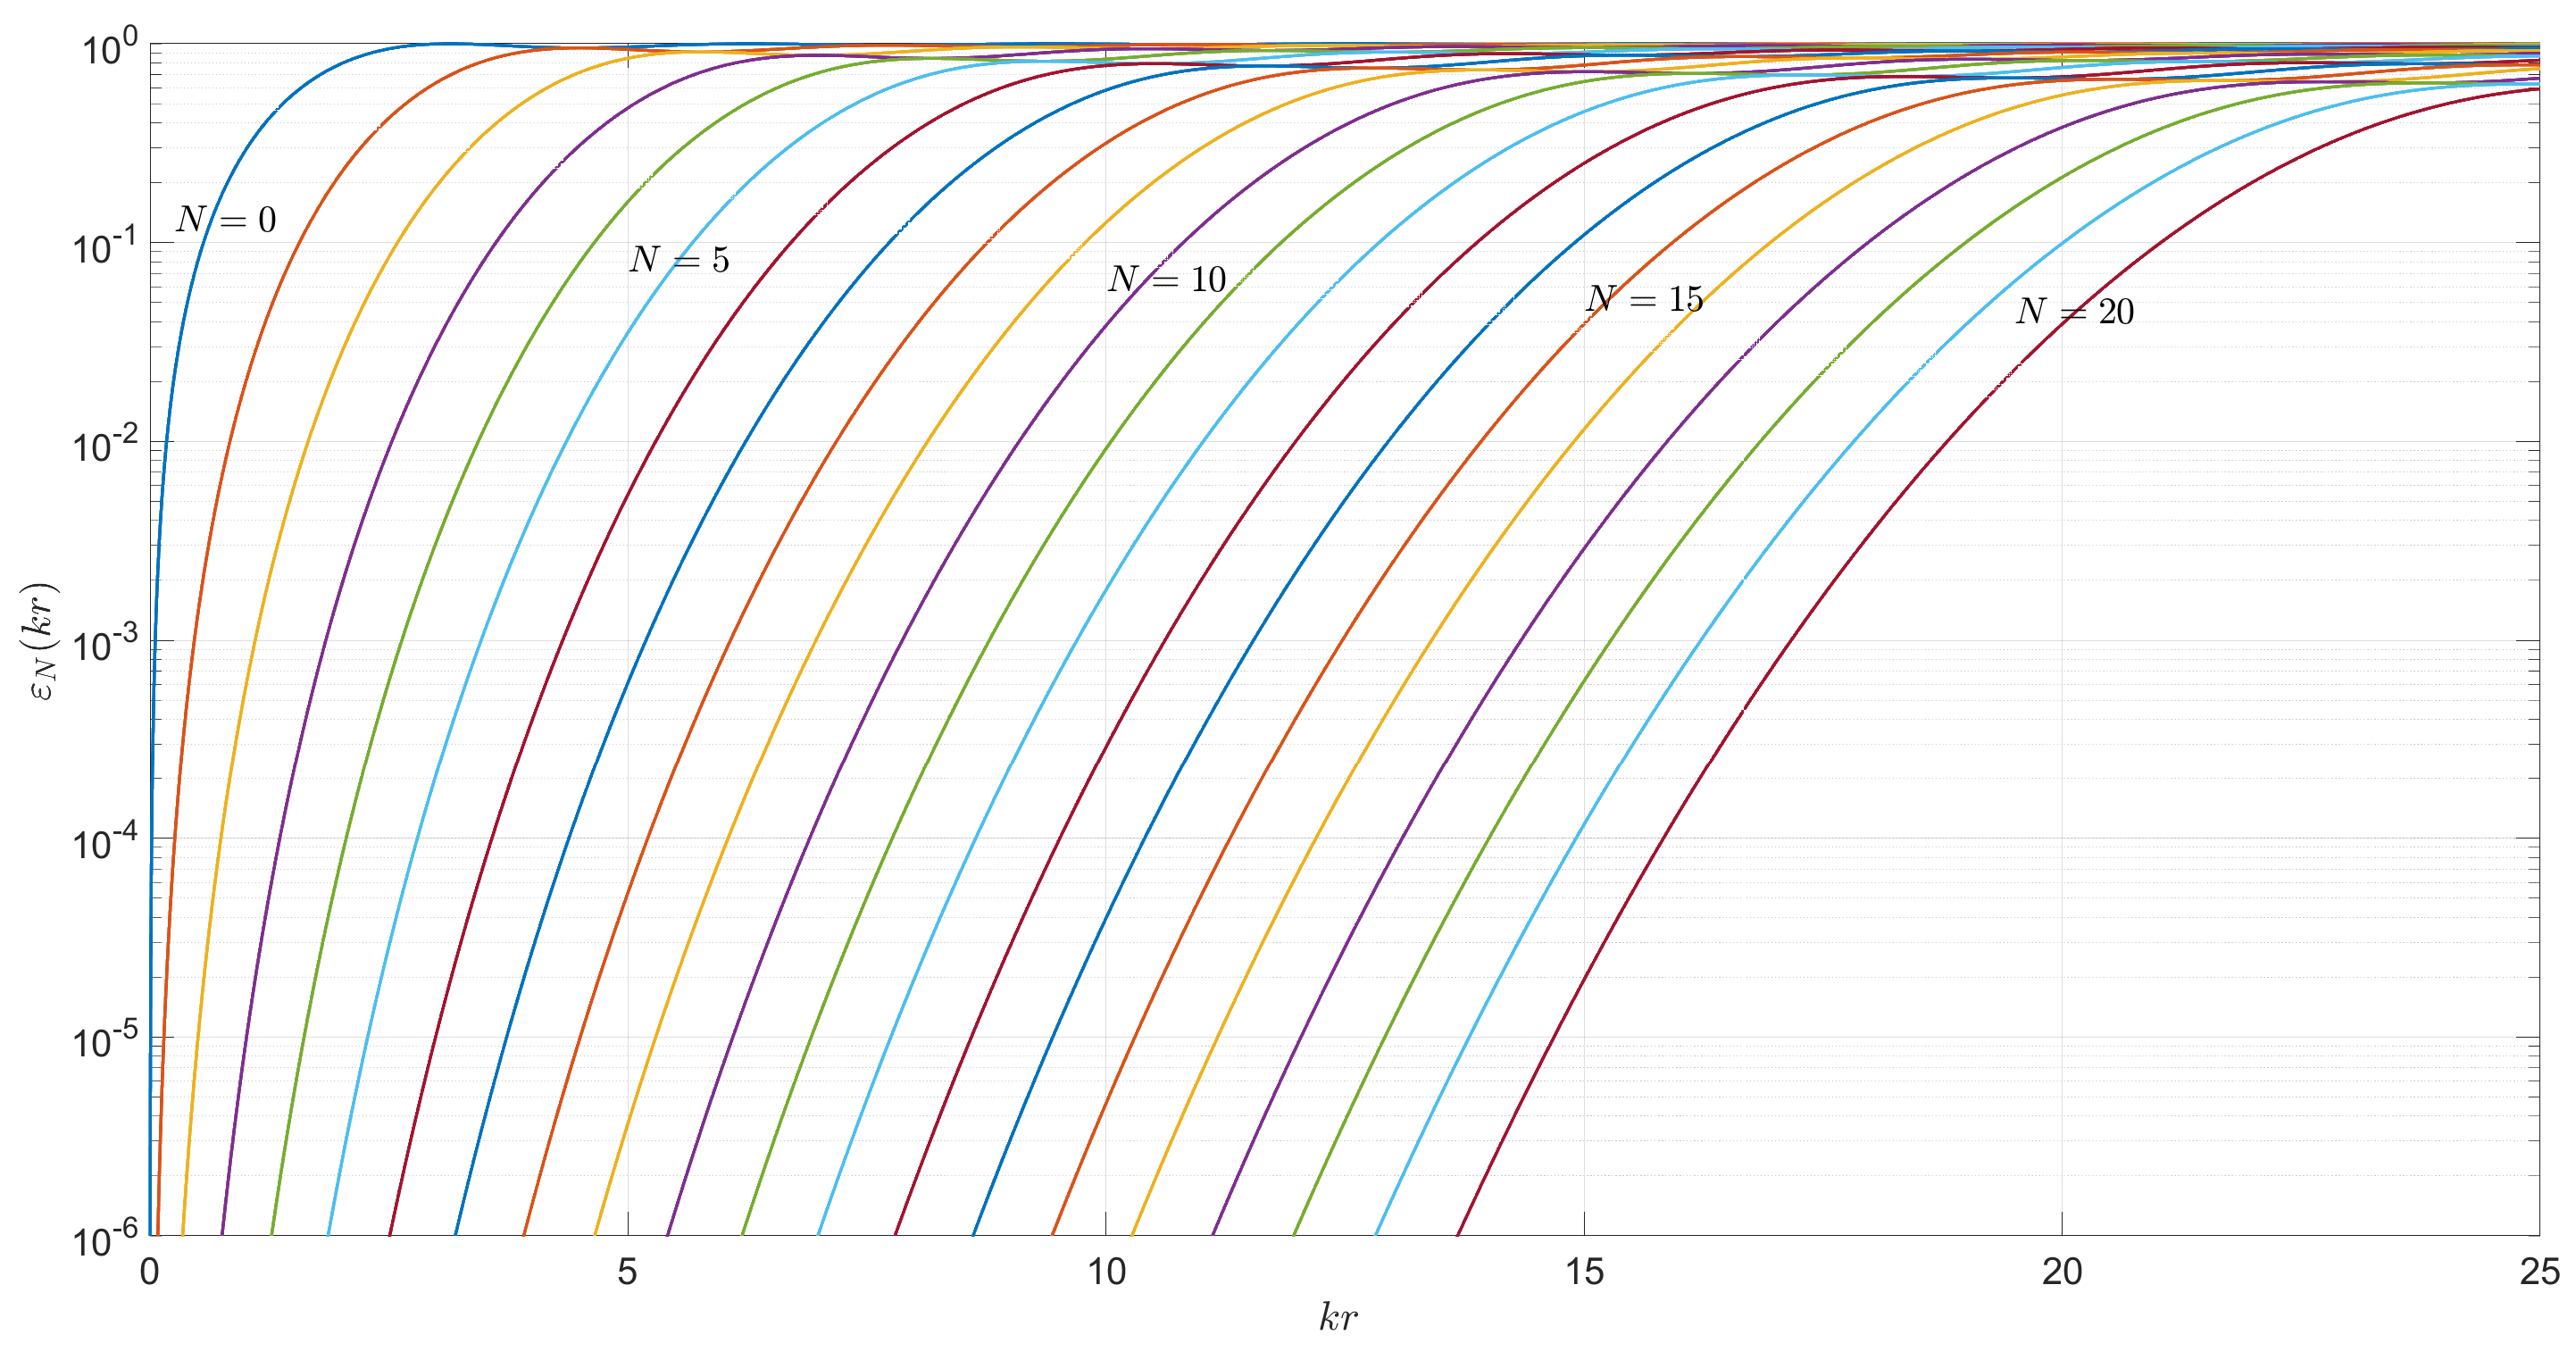
\includegraphics[width=0.9\textwidth]{figure/chapter2/N_kR.eps}
\caption{ 不同阶数~$N$~时归一化截断误差~$\varepsilon _N(kr)$~与~$kr$~的之间的关系}\label{Fig:N_kR}
\label{Fig:N_kR}
\end{figure}

在实际应用中,对于给定的频率~$k$、区域半径~$r$~以及可接受的误差,可以从图~\ref{Fig:N_kR}~查询所需要的分解阶次~$N$。以~$4\%$~的误差为例\tcite{Ward2001Reproduction}(对于大多数实际应用已经足够),可以看出频率~$k$、半径~$r$~和最低截断阶次~$N_{0}$~之间存在关系:
\begin{equation}\label{eq.krN}
   N_0=\lceil kr_0 \rceil,
\end{equation}
式中~$\lceil \cdot \rceil$~表示向上取整。

在半径小于~$r_0$~的重建区域内,重建声场可近似表示原始声场;在半径大于~$r_0$~的重建区域内,重建声场与原始声场差异较大,重建效果不准确。


\subsection{Ambisonics~解码}\label{Ambisonics_decoding}

Ambisonics~解码过程需要满足平面波声场的假设条件,扬声器均匀分布在球上,且只辐射平面波,实现扬声器阵列中心处的声场重建。
采用扬声器阵列重现声场的关键在于求取各个扬声器的激励信号,求解方法为使扬声器阵列产生的声场与原始平面波声场相匹配。原则上,通过使用~Ambisonics~分量信号的线性组合来导出扬声器信号,其中每个信号取决于扬声器相对于重建声场中心的实际位置。接下来从理论上对扬声器激励信号的求解过程进行推导。

由于假设扬声器只辐射平面波,参考式~\eqref{eq.coeS_planewave_N},使用~$L$~个位于~$(\theta_{l},\phi_{l})$~的扬声器进行声场重建时,所产生的线性叠加声场表示为:
\begin{equation}\label{eq.loudspeaker_array}
   \hat{P}(r,\theta,\phi,f)= \sum_{l=1}^{L} w_{l} \sum _{n=0}^{N} \sum _{m=-n}^n 4\pi i^{n} j_n(kr)\left[ Y_n ^m(\theta_{l},\phi_{l}) \right] ^{*} Y_n ^m(\theta,\phi),
\end{equation}
其中,$w_{l}$~为第~$l$~个扬声器的激励信号。

结合式~\eqref{eq.coeS_planewave_N}~和式~\eqref{eq.loudspeaker_array},建立扬声器阵列产生的总声场与原始平面波声场之间的等式:
\begin{equation}\label{eq.mode_matching}
   \sum_{l=1}^{L} w_{l} \left[ Y_n ^m(\theta_{l},\phi_{l}) \right] ^{*}  = \left[ Y_n ^m(\theta_{s},\phi_{s})\right] ^{*}.
\end{equation}

将式~\eqref{eq.mode_matching}~写为矩阵形式:
\begin{equation}\label{eq.min_error_odd_matrix}
\bm{\Psi w}=\bm{d},
\end{equation}
其中,$\mathbf{\Psi}$~是大小为~$(N+1)^2\times L$~的矩阵,其第~$v$~行~$l$~列元素~$\Psi_{v,l} = Y_{n}^{m}(\theta_{l},\phi_{l})$,其中~$v=n^2+n+m+1$,$\bm{w}$~是包含扬声器激励信号的矢量,
\begin{equation}\label{eq.matrix_a}
\bm{w} = [w_{1}~,~w_{2}~,~\cdots~,~w_{L}]^{T},
\end{equation}
\begin{equation}\label{eq.matrix_d}
\mathbf{d} = [Y_{0}^{0}(\theta_{s}~,~\phi_{s})~,\cdots,~Y_{n}^{m}(\theta_{s},\phi_{s})~,~\cdots~,~Y_{N}^{N}(\theta_{s},\phi_{s})]^{T}.
\end{equation}

由于扬声器阵列的配置方式是一定的,因此只有~$\bm{w}$~是未知量。根据球谐系数的数量~$(N+1)^2$~和扬声器的数量~$L$~之间的大小关系,对~$\bm{w}$~的求解分情况讨论~\tcite{Ward2001Reproduction,bookMatrix}:
\begin{compactitem}
\item 当~$L>(N+1)^2$~时,矩阵~$\bm{\Psi}$~是一个欠定矩阵,式~\eqref{eq.min_error_odd_matrix}~可能没有解,也可能有无穷多个解。$\bm{w}$~通常可以通过最小二乘问题求解:
    \begin{equation}
    \mathop{\min}_{\bm{w}} \| \bm{w} \|^{2}~~~\text{subject to}~~\bm{\Psi w = d}
    \end{equation}
    其中,$\| \cdot \|$~表示向量的~2~范数。
\item 当~$L=(N+1)^2$~时,矩阵~$\mathbf{\Psi}$~是一个非奇异方阵,式~\eqref{eq.min_error_odd_matrix}~有唯一解,采用矩阵求逆的方法求解~$\bm{w}$~:
    \begin{equation}
    \bm{w}_{\text{opt}} = \bm{\Psi}^{-1}\bm{d}.
    \end{equation}
\item 当~$L<(N+1)^2$~时,矩阵~$\bm{\Psi}$~是一个超定矩阵,式~\eqref{eq.min_error_odd_matrix}~没有准确解。$\bm{w}$~通常可以通过下式求解:
    \begin{equation}
    \mathop{\min}_{\bm{w}} \| \bm{\Psi w- d} \|^{2}
    \end{equation}

\end{compactitem}

并且在实际系统中,精确再现原始声场所需的扬声器数量为~$L\geq(N+1)^2$,即保证扬声器的数目大于需要约束的模态数~\tcite{Ward2001Reproduction}。

对于一阶~Ambisonics~来说,只包含零阶分量~$W$~和一阶分量~$X$~、$Y$~、$Z$,其扬声器激励信号也可以通过以下方式进行求解。
假设扬声器阵列均匀布放,且扬声器数目~$L\geq4$~,则扬声器激励信号为:
\begin{equation}
w_{l} = \bar{w}_{l}W + \bar{x}_{l}X + \bar{y}_{l}Y + \bar{z}_{l}Z,
\end{equation}
其中,
\begin{equation}
\begin{split}
\bar{w}_{l} & = \sqrt{2}/L \\
\bar{x}_{l} & = 3\cos\phi_{l}\cos\theta_{l}/L \\
\bar{y}_{l} & = 3\sin\phi_{l}\cos\theta_{l}/L \\
\bar{z}_{l} & = 3\sin\theta_{l}/L
\end{split}
\end{equation}



\subsection{虚拟扬声器方法}

在多通路环绕声系统中,为了产生空间中某一方向的虚拟源,并不一定需要在此方向布放一个扬声器,而是可以在空间中适当地布置若干个扬声器,通过调整各个扬声器的激励信号来产生不同方位的虚拟源。借鉴多通路环绕声系统,在双耳合成过程中,可以分别合成多个不同方位的虚拟扬声器,通过改变各个虚拟扬声器的激励信号,即可模拟出多通道声重放中不同虚拟源产生的双耳声信号。虽然这种双耳信号可能只是理想情况的低阶近似,但利用多声源综合定位的心理学原理,可在耳机重放中得到相应空间虚拟源的听觉感知~\tcite{jot1998approaches}\tcite{jot1999comparative}。这就是双耳合成中虚拟扬声器(virtual loudspeaker)方法的基本思路。 % 本段来源于《空间声原理》

由~\ref{Ambisonics_decoding}~节可以得到声场重现所需的虚拟扬声器摆放方式和对应的扬声器激励信号,为了让~Ambisonics~系统可以用于耳机实现,我们需要对虚拟扬声器信号加以~HRTF~渲染,该方法可以消除听音空间对扬声器回放产生的影响。

假设整个空间中有~$L$~个虚拟声源(虚拟扬声器),其位置为~$(\theta_{l},\phi_{l})$,激励信号为~$w_{l}(f)$,双耳接收到的信号是多个声源共同作用的结果:
\begin{equation}\label{eq.loudspeaker_to_headphone}
\begin{split}
B_{\text{L}}(f) = \sum_{l=1}^{L}H_{\text{L}}(\theta_{l},\phi_{l},f)w_{l}(f)\\
B_{\text{R}}(f) = \sum_{n=l}^{L}H_{\text{R}}(\theta_{l},\phi_{l},f)w_{l}(f),
\end{split}
\end{equation}
其中,$H_{\text{L}}(\theta_{l},\phi_{l},f)$~和~$H_{\text{R}}(\theta_{l},\phi_{l},f)$
是声源位于~$(\theta_{l},\phi_{l})$~处的左、右耳~HRTF~数据。
最后对~$B_{\text{L}}(f)$~和~$B_{\text{R}}(f)$~求反傅里叶变换即可得到时域双耳信号。

但是基于~Ambisonics~的虚拟扬声器方法会带来一些问题:一是不同的虚拟扬声器数目和位置会对所获取的双耳信号带来影响,二是扬声器所在位置的声像会不可避免地被加重。并且当扬声器所处方位在现有的~HRTF~数据库中没有对应的数据,此时需要对原始~HRTF~进行插值。

\section{基于球谐分解的双耳渲染算法}\label{sec.SHdecomposition}

近年来,基于球谐分解的双耳渲染算法受到人们的广泛关注。其核心思想是不仅对声场进行球谐分解,同时对~HRTF~进行球谐分解,直接在球谐域上进行渲染。可以避免了虚拟扬声器引入对双耳信号带来的影响。

对声场使用球谐函数进行表示:
\begin{equation}
S(r,\theta,\phi,f) = \sum_{n=0}^{N_{s}}\sum_{m=-n}^{n} S_n^m(r,f)Y_{n}^{m}(\theta,\phi),
\end{equation}
其中,$S_n^m(r,f)$~是声学场景的球谐系数,无需声源信号和方位的先验信息。$N_{s}$~为声场的球谐分解阶次,由录制设备决定。

HRTF~一般在一个固定的球面上进行多点采样,当球面半径大于~1~米时,可以认为是远场~HRTF~,可以使用球谐函数进行分解:
\begin{equation}\label{HRTF_decomposition}
\begin{split}
H_{\text{L}}(\theta,\phi,f) & = \sum_{n=0}^{N_{h}}\sum_{m=-n}^{n} \beta_{nm}^{\text{L}}(f)Y_{n}^{m}(\theta,\phi) \\
H_{\text{R}}(\theta,\phi,f) & = \sum_{n=0}^{N_{h}}\sum_{m=-n}^{n} \beta_{nm}^{\text{R}}(f)Y_{n}^{m}(\theta,\phi),
\end{split}
\end{equation}
其中,$N_{h}$~是~HRTF~进行球谐分解的阶数。

由于声源可能具有一定体积,例如面源、体源,并且房间混响会产生反射,因此假设声场中声源是连续分布的,则左耳的信号可以表示为~\tcite{Benesty2008Microphone}\tcite{2013Study}\tcite{2016Fundamentals}:
\begin{align}
B_{\text{L}}(f) &= \int_{0}^{2\pi}\int _{0}^{\pi}S(r,\theta,\phi,f)\left[H_{\text{L}}(\theta,\phi,f)\right]^{*}\sin \theta d\theta d\phi \nonumber \\
&= \int_{0}^{2\pi}\int _{0}^{\pi} \sum_{n=0}^{N_{s}}\sum_{m=-n}^{n} S_n^m(r,f)Y_{n}^{m}(\theta,\phi) \left[  \sum_{n'=0}^{N_{h}}\sum_{m'=-n'}^{n'} \beta_{n'm'}^{\text{L}}(f)Y_{n'}^{m'}(\theta,\phi)\right]^{*}
\sin\theta d\theta d\phi \nonumber \\
&=\sum_{n=0}^{N_{s}}\sum_{m=-n}^{n} \sum_{n'=0}^{N_{h}}\sum_{m'=-n'}^{n'} S_n^m(r,f)\left[\beta_{n'm'}^{\text{L}}(f)\right]^{*}
\int_{0}^{2\pi}\int _{0}^{\pi} Y_{n}^{m}(\theta,\phi)\left[Y_{n'}^{m'}(\theta,\phi)\right]^{*}\sin\theta d\theta d\phi \nonumber \\
&= \sum_{n=0}^{N}\sum_{m=-n}^{n} S_n^m(r,f)\left[\beta_{nm}^{\text{L}}(f)\right]^{*},
\label{eq.BL}
\end{align}
其中,$N=\min \left\{ N_{s},N_{h} \right\}$,最后一个等式的推导借助了球谐函数的正交性,如式~\eqref{eq.orth}~所示。

同理,右耳信号可以表示为:
\begin{equation}
B_{\text{R}}(f) = \sum_{n=0}^{N}\sum_{m=-n}^{n} S_n^m(r,f) \left[ \beta_{nm}^{\text{R}}(f)\right]^{*}
\label{eq.BR}
\end{equation}


由~$N=\min \left\{ N_{s},N_{h} \right\}$~可知,在球谐域上进行双耳渲染时的球谐阶次由声场和~HRTF~进行球谐分解的阶次共同决定。HRTF~数据库的球面采样点较为密集,可以实现高阶球谐系数的获取,并且研究表明,要想对高达~15~kHz~的~HRTF~进行精确的物理表征,大约需要~$N_{h}= 34$~的阶次。声场方面,要想准确获取~$N$~阶声场,至少需要~$(N+1)^2$~个采样点,其详细推导见第~\ref{section_microphone_array_coe}~节,而实际系统中,对~$N_{h}=34$~对应的~1225~个通道的采集、传输和处理很难实现,一般来说录制设备的通道数较少,所能准确获取的声场系数的阶次较低,基本满足~$N_{s}<5$~\tcite{2018Binaural}。
二者之间的阶次存在不匹配问题,HRTF~虽然可以获取高阶球谐分量,但也只能使用低阶进行表示。HRTF~的直接低阶截断会导致高频能量损失,带来一定的误差。除此之外,还存在其他问题,例如录音设备的尺寸小于人头尺寸,录音设备的采样率与~HRTF~数据库采样率不一致等。
这些不匹配问题将会导致所获取的双耳信号的空间分辨率受限、定位线索(双耳时间差~ITD、双耳声级差~ILD)的损伤、空间感的下降等,直接影响声源方位的感知、外化~(externalization)、感知声源宽度和音色等~\tcite{sheaffer2014rendering}\tcite{2013Spatial}\tcite{2015Efficient}\tcite{2017equalization}。


本文主要针对以上问题,对基于球谐分解的双耳渲染算法进行研究,对头相关传递函数~HRTF~的预处理加以研究,并且从另外一个方面~——~声场出发,提出改进方法。

\newpage
\section{本章小节}
本章主要介绍了几种常见的双耳渲染技术及其原理。 首先对基于~HRIR~和~BRIR~的虚拟听觉的方法进行了简单介绍,其中头相关传递函数~HRTF~是所有双耳渲染算法中的核心数据。接下来对基于~Ambisonics~的虚拟扬声器方法进行了详细推导,其核心思想是对声场的球谐分解,再利用各阶谐波分量求解重建声场所需的扬声器设置和对应的激励信号,最后结合虚拟扬声器获取双耳信号,其中对声场进行正交球谐分解是本文的重要理论基础。最后对基于球谐分解的双耳渲染技术进行了介绍和理论推导,并对其所存在的问题进行了简单描述,本文将在此算法框架下进行,针对其所存在的问题,提出改进算法。
%Binaural Reproduction of Plane Waves With
%Reduced Modal Order
%
%Binaural rendering of Ambisonic signals by head-related impulse response time
%alignment and a diffuseness constraint
%
%HRTF——Note
%
%Insights into head-related transfer function: Spatial
%dimensionality and continuous representation
%
%可以参考: Interaural cross correlation in a sound field represented by spherical harmonics
%里面包括了双耳信号获取和HRTF分量求解。 已下载,已打印,other标号。

\chapter{基于~HRTF~球谐分解的双耳渲染算法} \label{chapter.HRTF}

对~HRTF~进行球谐分解并在球谐域上直接渲染的双耳渲染算法近年来得到了广泛关注,本章将在~\ref{sec.SHdecomposition}~节的基础上对其进行详细介绍,其包含两个同等重要的部分:声场和~HRTF。在声场获取方面,麦克风阵列尤其是球形麦克风阵列可以更好地采集声场的特征,具有高质量、高保真的录制效果,是多通道录制与重构、空间音频技术的重要工具。首先对空心球和刚性球进行讨论和对比,分别给出其球谐系数的求解方法。接下来对~HRTF~的获取和其球谐分量的求解方法进行介绍。并且在此基础上,对~HRTF~的预处理方法的原理进行详细介绍,该方法可以有效降低~HRTF~的球谐分解阶次。最后通过实验验证了预处理方法的有效性。

\section{球形麦克风阵列的声场录制及球谐系数估计}\label{section_microphone_array_coe}
声场录制的关键在于如何准确获得待录制声场的高阶球谐系数,使用球形麦克风阵列可以实现此目标。球形麦克风阵列是通过将麦克风放置在三维空间中并记录麦克风所在位置的声压信号来实现的。影响球阵可以准确重现声场的因素包括频率、阵列半径、阵元数目和球面采样方式等~\tcite{SMA_design}。
录制声场球谐系数的估计依赖于麦克风阵列的采样配置,在一些特殊的采样方式~\tcite{rafaely_fundamentals_2019}~例如等角采样、高斯采样和均匀采样(如图~\ref{fig:sampling}~所示)的情况下,可以使用求和来代替积分计算录制声压的球谐系数,能够方便地计算函数的球傅里叶变换。在实际系统中很难要求所有球阵满足特殊的采样方式,因此需要给出在任意采样配置下使用球傅里叶变换来计算球谐系数的方法。

\begin{figure}[!h]
\centering
\includegraphics[width=0.85\textwidth]{figure/chapter3/sampling-eps.pdf}
\caption{ 球面采样:(a)~等角采样;
(b)~高斯采样;(c)~均匀采样。}\label{fig:sampling}
\end{figure}

%%%%%%%%%%%%%%%%%%%%% 开球和刚性球 %%%%%%%%%%%%
使用半径为~$R$~的球形麦克风阵列采集来自~$(\theta_s,\phi_s)$~的单位幅度平面波时,麦克风~$(\theta _q,\phi _q)$~ 连续分布在球面上。此处假设声源均位于球形麦克风阵列外,麦克风观测声压可分为空心球和刚性球两种情况进行讨论~\tcite{williams_fourier_2000,rafaely_fundamentals_2019}。

\subsection{空心球的球谐系数估计}

对于空心球来说,忽略单个麦克风和支架对声波的影响,可以认为其录制的声场即为真实环境下的声场,直接进行球谐系数的估计。

对于特殊的采样方式,球面积分可以通过~$Q$~个球面采样~$(\theta_{q},\phi_{q})$~的加权求和来逼近,如式~\eqref{eq.sum_integral}~所示:
\begin{equation}\label{eq.sum_integral}
   \int_{0}^{2\pi}\int _{0}^{\pi} g(\theta,\phi) \sin\theta d\theta d\phi \approx \sum_{q=1}^{Q} \alpha_{q} g(\theta_{q},\phi_{q}),
\end{equation}
其中,$\alpha_{q}$~是采样权重,式~\eqref{eq.Equal_angle_sampling}、\eqref{eq.Gaussian_sampling}~和~\eqref{eq.uniform_sampling}~分别为等角采样、高斯采样和均匀采样下的权重表达式:
\begin{equation}\label{eq.Equal_angle_sampling}
\alpha_{q}=\frac{2 \pi}{(N+1)^{2}} \sin \left(\theta_{q}\right) \sum_{q^{\prime}=0}^{N} \frac{1}{2 q^{\prime}+1} \sin \left(\left[2 q^{\prime}+1\right] \theta_{q}\right).
\end{equation}
\begin{equation}\label{eq.Gaussian_sampling}
\alpha_{q}=\frac{\pi}{N+1} \frac{2\left(1-\cos ^{2} \theta_{q}\right)}{(N+2)^{2}\left[P_{N+2}\left(\cos \theta_{q}\right)\right]^{2}}.
\end{equation}

\begin{equation}\label{eq.uniform_sampling}
   \alpha_{q} = \frac{4\pi}{Q}.
\end{equation}

则通过球傅里叶变换获取球谐系数的式~\eqref{eq.SFT}~可以表示为:
\begin{equation}\label{eq.sample_coe}
   S_n ^m(r,f)=\sum_{q=1}^{Q} \alpha_{q} S(r,\theta_{q},\phi_{q},f)[{Y_n^{m}(\theta_{q},\phi_{q})}]^{*}.
\end{equation}
此时,球谐系数可以直接采用上式进行求解。

在某些情况下,从这些或其他预定义的采样配置中选择采样集可能是不可行的,例如,由于麦克风定位的机械限制。因此,在任意给定采样集时,如何计算球面球谐系数在实际应用中具有重要的价值。考虑在单位球面上进行采样,根据球傅里叶变换,第~$q$~个麦克风的接收信号可以写为:
\begin{equation}\label{eq.coe_random_sampling}
   S(r,\theta_{q},\phi_{q},f)=\sum _{n=0}^{N_{s}}\sum _{m=-n}^n S_n ^m(r,f)Y_n ^m(\theta,\phi),
\end{equation}
其矩阵形式为:
\begin{equation}\label{eq.coeMat_random_sampling}
\bm{S}=\bm{Y S_{nm}},
\end{equation}
其中,$\bm{S}$~和~$\bm{S_{nm}}$~是长度为~$Q$~和~$(N_{s}+1)^2$~的列向量,$\bm{Y}$~是大小为~$Q\times(N_{s}+1)^2$~的矩阵,
\begin{equation}
\bm{S} = [S(r,\theta_{1},\phi_{1},f),~S(r,\theta_{2},\phi_{2},f)~,~\cdots~,~S(r,\theta_{Q},\phi_{Q},f)]^{T},
\end{equation}
\begin{equation}
\bm{S_{nm}} = [S_{0}^{0}~,\cdots,~S_{n}^{m}~,~\cdots~,~S_{N_{s}}^{N_{s}}]^{T},
\end{equation}

\begin{equation}
\bm{Y}=\left[
\begin{array}{ccccc}
Y_{0}^{0}\left(\theta_{1}, \phi_{1}\right) & \cdots & Y_{n}^{m}\left(\theta_{1}, \phi_{1}\right) & \cdots & Y_{N_{s}}^{N_{s}}\left(\theta_{1}, \phi_{1}\right) \\
Y_{0}^{0}\left(\theta_{2}, \phi_{2}\right) & \cdots &  Y_{n}^{m}\left(\theta_{2}, \phi_{2}\right) & \cdots & Y_{N_{s}}^{N_{s}}\left(\theta_{2}, \phi_{2}\right) \\
\vdots  & \ddots & \vdots  & \ddots & \vdots \\
Y_{0}^{0}\left(\theta_{Q}, \phi_{Q}\right) & \cdots & Y_{n}^{m}\left(\theta_{Q}, \phi_{Q}\right) & \cdots & Y_{N_{s}}^{N_{s}}\left(\theta_{Q}, \phi_{Q}\right)
\end{array}\right].
\end{equation}

当~$Q=(N+1)^2$~时,式~\eqref{eq.coeMat_random_sampling}~的解可以通过矩阵~$\bm{Y}$~的逆求解(要求球形麦克风阵列的采样位置满足矩阵~$\bm{Y}$~可逆的条件):
\begin{equation}
\bm{S_{nm}} = \bm{Y}^{-1}\bm{S},
\end{equation}
在许多情况下都使用过采样,即~$Q>(N+1)^2$,此时式~\eqref{eq.coeMat_random_sampling}~超定,其最小二乘解由矩阵的伪逆给出::
\begin{equation}
\bm{S_{nm}} = \bm{Y^{\dagger}} \bm{S}= (\bm{Y}^{H}\bm{Y})^{-1}\bm{Y}^{H}\bm{S}.
\end{equation}
当~$Q<(N+1)^2$~时,采样点数不足,式~\eqref{eq.coeMat_random_sampling}~可能不能提供正确的解。

\subsection{刚性球的球谐系数估计}

和空心球相比,刚性球录制的总声压场,也就是实验中的被测声压,可以分为入射声场和散射声场两个部分。从实验的角度来说,入射声场是针对球体不存在时测量的声压场,而散射声场是球体存在时声压场的变化量。对于刚性球来说,其表面的径向速度为~0,即球体表面处入射场和散射场的总径向速度为~0,满足~Neumann~边界条件~\tcite{williams_fourier_2000}。如果散射场为零,则认为该球体是完全可透射的。
% 对于释压球来说,其在球体表面上的总声压为~0。

大多数散射问题的研究都是从平面波着手的,对于来波方向为~$(\theta_s,\phi_s)$~的单幅度平面波来说,麦克风~$(r,\theta _q,\phi _q)$~处观测到的入射声压(直达声)可以用球贝塞尔函数表示:
\begin{equation}  \label{SMic_pressure open}
   S_{\mathrm{dir}}(r,\theta _q,\phi _q,f)=\sum _{n=0}^{\infty}4\pi i^n j_n(kr)\sum _{m=-n}^{n}[Y_n ^{m}(\theta_s,\phi_s)]^*Y_n ^{m}(\theta_q,\phi_q).
\end{equation}
上式即为空心球情况下麦克风的接收信号。

因为散射声场代表了入射声波在球面的散射而发出的球面声波,因此散射声压可以利用表示去波的第一类球汉克尔函数展开:
\begin{equation}  \label{SMic_pressure scat}
   S_{\mathrm{scat}}(r,\theta _q,\phi _q,f)=-\sum _{n=0}^{\infty}4\pi i^n \frac{j'_n (kr)}{({h^{(1)}_n})'(kr)}h_n^{(1)}(kr)\sum _{m=-n}^{n}[Y_n ^{m}(\theta_s,\phi_s)]^*Y_n ^{m}(\theta _q,\phi _q),
\end{equation}
其中,$j_n'(kr)$~和~$({h^{(1)}_n})'(kr)$~分别为~$n$~阶球贝塞尔函数~$j_n(kr)$~和~$n$~阶第一类球汉克尔函数~$h_n^{(1)}(kr)$~的导数。波动方程在频域上的表示称为亥姆霍兹方程,球坐标系下亥姆霍兹方程中只与距离相关的项所构成的方程被称为球贝塞尔方程,球贝塞尔函数和球汉克尔函数共同组成了球贝塞尔方程的解。

对于刚性球来说,麦克风的录制信号中除了直达声外,还包含因球面散射形成的散射声,则接收到的总声压可表示为:
\begin{align}  \label{SMic_pressure rigid}
   S(r,\theta_q,\phi_q,f)&= S_{\mathrm{dir}}(r,\theta_q,\phi_q,f)+S_{\mathrm{scat}}(r,\theta_q,\phi_q,f)   \nonumber \\
   &=\sum _{n=0}^{\infty} 4\pi i^n \left( j_n(kr)-\frac{j'_n (kr)}{({h^{(1)}_n})'(kr)}h_n^{(1)}(kr) \right) \sum _{m=-n}^{n}[Y_n ^{m}(\theta_s,\phi_s)]^*Y_n ^{m}(\theta_q,\phi_q),
\end{align}

整合公式~\eqref{SMic_pressure open}~和式~\eqref{SMic_pressure rigid},可以得到采用不同麦克风阵列时,第~$q$~个麦克风接收信号的表达式:
\begin{equation}  \label{SMic_pressure}
   S(r,\theta_q,\phi_q,f)=
   \sum _{n=0}^{\infty} b_n(kr) \sum _{m=-n}^{n}[Y_n ^{m}(\theta_s,\phi_s)]^*Y_n ^{m}(\theta_q,\phi_q),
\end{equation}
其中,$b_n$~表示模态强度:
\begin{equation}\label{eq.bn(kr)}
b_n(kr) =
\begin{cases}
 4\pi i^n j_n(kr)  & ~\mbox{空心球} \\
 4\pi i^n \left(j_n(kr)-\frac{j'_n (kr)}{({h^{(1)}_n})'(kr)}h_n^{(1)}(kr) \right) & ~\mbox{刚性球}.
\end{cases}
\end{equation}


\begin{figure}[H]
\centering
\subfigure[]{
\includegraphics[width=0.48\textwidth]{figure/chapter3/bn_open}}
\hfill
\subfigure[]{
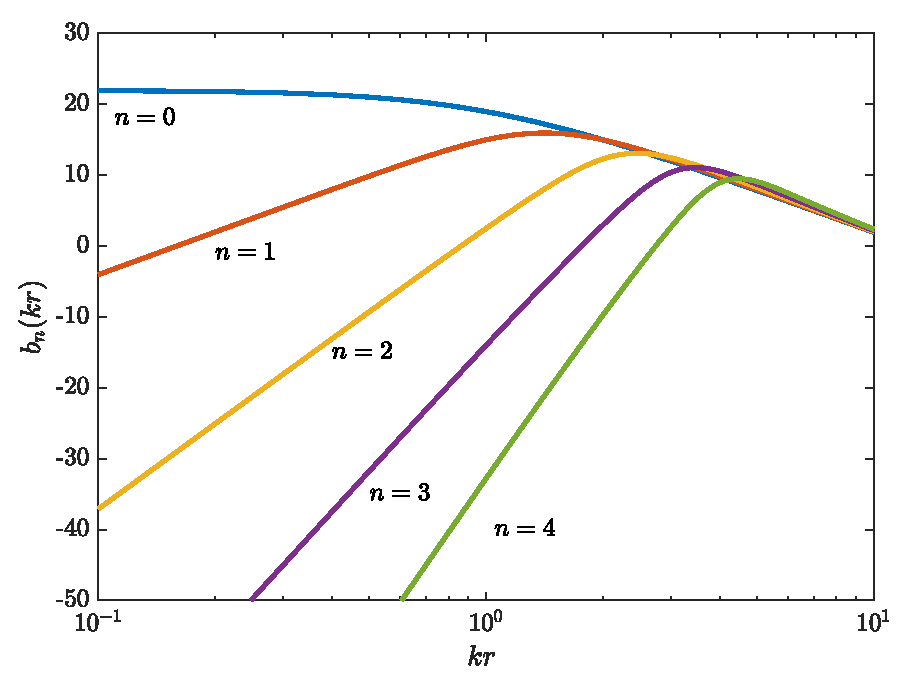
\includegraphics[width=0.48\textwidth]{figure/chapter3/bn_rigid}}
\caption{模态强度~$b_n$:(a)~空心球模态强度; (b)~刚性球模态强度}
\label{fig:bn}
\end{figure}

图~\ref{fig:bn}~为模态强度~$b_n$~随~$kr$~的变化趋势图。(a)~中曲线有很深的凹陷,即在某些频率处模态强度为~0。而~(b)~中刚性球可以避免空心球所带来的凹陷(零点)问题,这是因为刚性球麦克风接收到的不仅包含直达声还有声波入射到球体产生的散射声。关于零点问题带来的影响将在第~\ref{sec.modelAndMusic}~节中关于球谐域~MUSIC~定位算法和第~\ref{subsec.open_rigid}~节中的实验结果进行展现。

并且由于散射声场的存在,在高阶次和低频率的情况下,刚性球模态强度的幅度稍大于空心球,因此刚球对传感器噪声和其他误差的影响的鲁棒性有些许提升~\tcite{rafaely_fundamentals_2019}。另外,实际情况下由于麦克风数目较多,所以做成刚性球更合理,目前常用的刚球为~32~通路~Eigenmike~\tcite{microphone}。

%在求解刚性球录制声场的球谐分量时,在根据式~\eqref{eq.coe_random_sampling}~计算得到~$S_n ^m(r,f)$~之后需要一定的转换,以避免球面散射带来的影响。
%
%\begin{equation}\label{eq.coe_eigen}
%S_{nm}^{rigid}(r,f) = \frac{ S_n^m(r,f) }{j_n(kr)-\frac{j'_n (kr)}{[{h^{(1)}_n}]'(kr)}h_n^{(1)}(kr) } j_n(kr)
%\end{equation}
%
%通过式~\eqref{eq.coe_eigen}~即可求解原始无刚球情况下的球谐分量。

\section{~HRTF~的球谐分解}\label{sec.SHcoe_HRTF}

本节将对头相关传递函数~HRTF~的三种获取方式以及本文所采用的两种数据库加以介绍,并且给出了如何从给定~HRTF~数据库中求解~HRTF~球谐系数的方法。


\subsection{HRTF~的获取}
HRTF~和~HRIR~是双耳渲染算法中合成双耳信号的重要数据基础,其可以通过计算、定制与测量三种方法获取~\tcite{book_xiebosun}。

原则上,声波经由头部、耳廓、躯干等生理结构的综合滤波过程可以通过求解加以边界条件约束的波动方程来获得,即边界元法(boundary element method,BEM)\tcite{katz2001boundary}。但实际上边界表面的不规则性会产生及其复杂的现象,以足够的准确度实现边界表面(尤其是耳廓)的测量具有一定的挑战,并且计算量较大。还有一些分析解决方案适用于非常简单的几何形状,在简化情况下,忽略耳廓和躯干的影响,将头部近似为刚性球体。在此基础上,雪人模型~\tcite{algazi2002approximating}~将头部和躯干简化为两个不同半径的球,并采用多重散射或多级展开的方法进行求解,数学方法非常复杂。目前已知的仿真~HRTF~数据库为~MESH2HRTF~\tcite{HRTF_MESH2HRTF},其采用边界元法,频率范围为~100Hz~到~22kHz,以~100Hz~为间隔,球面采样点数为~4334~个,采样方式为列别捷夫采样。

~HRTF~的定制主要应用于获取个性化~HRTF~,假定~HRTF~和一定的生理参数之间存在高的相关性。主要包括生理参数匹配法、频率标度变换法和生理参数线性回归法,近几年也出现了基于机器学习的个性化~HRTF~生成模型。总体上,定制~HRTF~较测量和计算来说比较简单,且可以得到一定的效果,但其准确性有待进一步改进~\tcite{book_xiebosun}。% (摘自《空间声原理》)

现有的技术中,实验测量是获得~HRTF~最重要且最准确的手段~\tcite{book_xiebosun},一个扬声器在特定的位置产生一个脉冲或其他宽带信号,然后通过记录放置在人工头或真人受试者耳道内的两个麦克风的输出信号来测量。根据~HRTF~的定义,理想情况下的测量应该在自由场(消声室)的环境下进行,但实际中也经常采用非消声室的测量方法,为了避免环境反射声的影响,会加以时间窗处理。

双耳麦克风的尺寸很小可以放置在耳道入口处,并使用泡沫环保持在适当的位置,这被称为封闭耳道法,进入耳道的信号被麦克风捕获并存储为双通道录音。封闭耳道法经常用于~HRTF~的测量~\tcite{book_immersive}。

目前国际上已有许多课题组对人工头和真人受试者的远场~HRTF/HRIR~进行了测量,建立了相应的数据库~\tcite{book_xiebosun},大多数数据库都是在远场条件下进行测量,但也有部分是在近场进行。
现有的较为常用的远场~HRTF~数据库包括~MIT~数据库~\tcite{hrtf_MIT}~和~CIPIC~数据库~\tcite{hrtf_CIPIC},其对应的数据已在网上公开。
% (http://sound.media.mit.edu/resources/KEMAR.html~和~http://www.ece.ucdavis.edu/cipic/spatial-sound/hrtf-data)。

除此之外,Benjamin~Bernschutz~使用~Neumann~KU-100~建立了一个远场~HRTF~数据库~\tcite{Benjamin2013A},测量环境为消声室,共采用了~4~种球面采样方式,包括在以~$1^{\circ}$~为角度间隔的圆周上均匀采样,2354、2702~点球面列别捷夫采样和以~$2^{\circ}$~为间隔的球面高斯采样(共计~16020~个采样点),此数据库将在第~\ref{sec.Pre_result}~节用于体现~HRTF~预处理的结果展示。


本文主要采用~CIPIC~数据库进行双耳渲染,其来自加州大学戴维斯分校~CIPIC~交互实验室。在非消声室环境下,对~43~名真人受试者(27~男,16~女)进行测量,是目前真人~HRTF~数据库中空间分辨率较高,同时受试者人数较多的一个,同时给出了真人受试者的生理尺寸~\tcite{book_xiebosun}。
其测量环境为非消声室环境,测量方法为封闭耳道法,~HRIR~的长度为~200~点,采样频率为~44.1~kHz。其测量时采用双耳极坐标系统,如图~\ref{fig:CIPIC_location}~(a)~所示,其中,$(\varTheta,\varPhi) = (0^{\circ},0^{\circ})$~为正前方,$(\varTheta,\varPhi) = (90^{\circ},0^{\circ})$~为正右方。

\begin{figure}[H]
\centering
\subfigure[]{
\includegraphics[width=0.3\textwidth]{figure/chapter3/binaural_cor}}
\hfill
\subfigure[]{
\includegraphics[width=0.6\textwidth]{figure/chapter3/cipic}}
\caption{CIPIC~数据库角度说明:(a)~双耳极坐标系~\tcite{book_xiebosun},(b)~声源位置分布}
\label{fig:CIPIC_location}
\end{figure}

如图~\ref{fig:CIPIC_location}~(b)~所示,CIPIC~数据库共包括~1250~个测量位置,50~个俯仰角为~$\varTheta = -45^{\circ}+5.625^{\circ}\times (0:1:49)$,每个俯仰角均对应~25~个方位角,且非均匀分布,其设定为:
\begin{equation*}
\left[-80~-65~-55~-45:~5:~45~~55~~65~~80\right]
\end{equation*}


以~003~号受试者为例,当声源位于水平面且方位角为~$80^{\circ}$~时,即声源位于右耳方向附近,左右耳的~ITD~和~ILD~取接近最大值,对应的左、右耳的~HRIR~和~HRTF~如图~\ref{fig:CIPIC_80du}~所示。
方位角为~$0^{\circ}$~时,即声源位于正前方,如图~\ref{fig:CIPIC_80du}~所示。

\begin{figure}[H]
\centering
\subfigure[]{
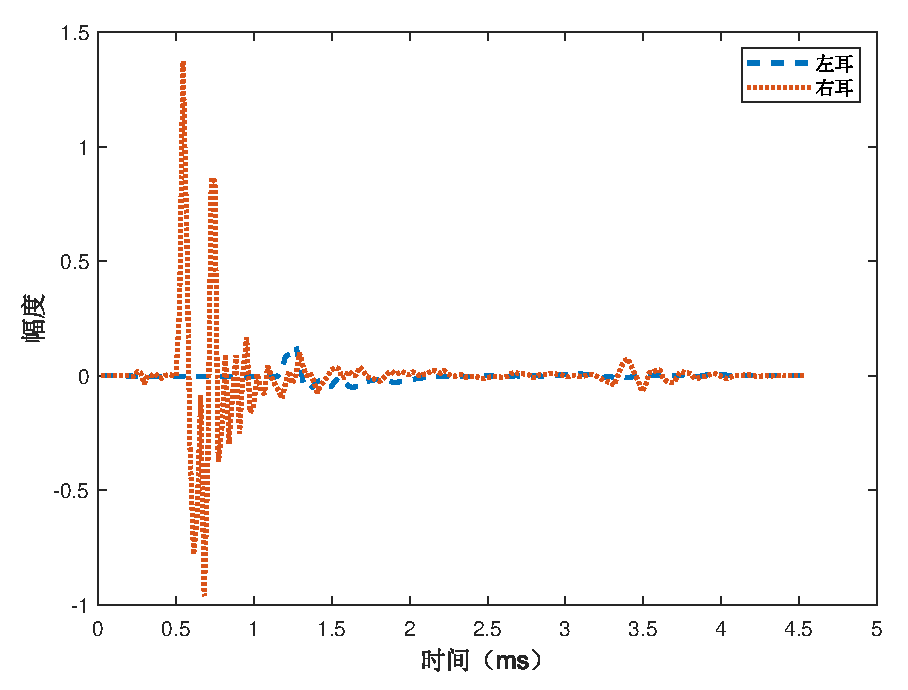
\includegraphics[width=0.48\textwidth]{figure/chapter3/80du_HRIR}}
\hfill
\subfigure[]{
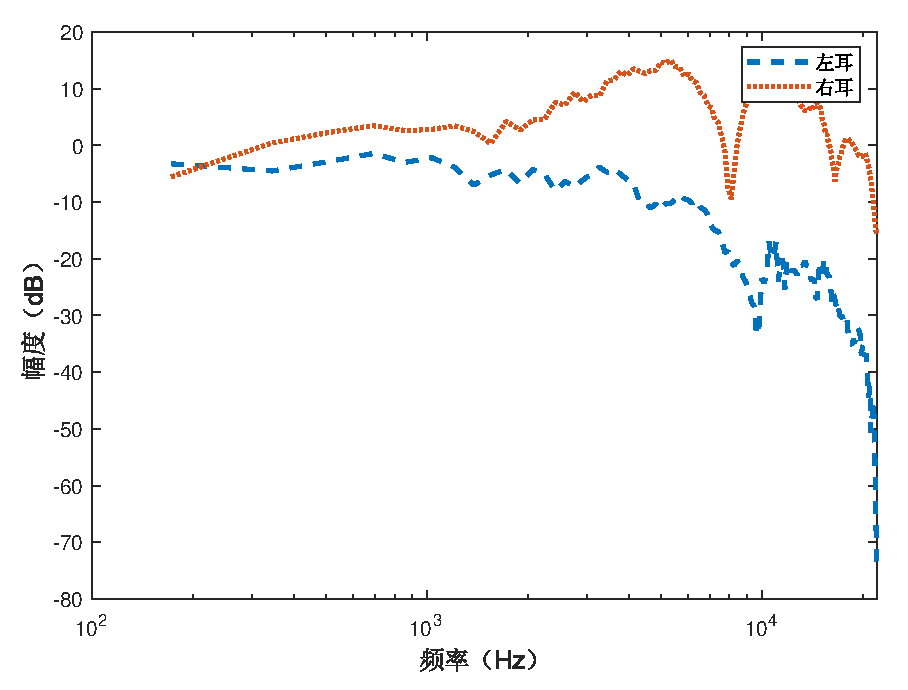
\includegraphics[width=0.48\textwidth]{figure/chapter3/80du_HRTF}}
\caption{CIPIC~数据库中声源位于水平面且方向为~$80^{\circ}$~时的左右耳~HRIR~和~HRTF~数据:(a)~HRIR,(b)~HRTF}
\label{fig:CIPIC_80du}
\end{figure}

\begin{figure}[H]
\centering
\subfigure[]{
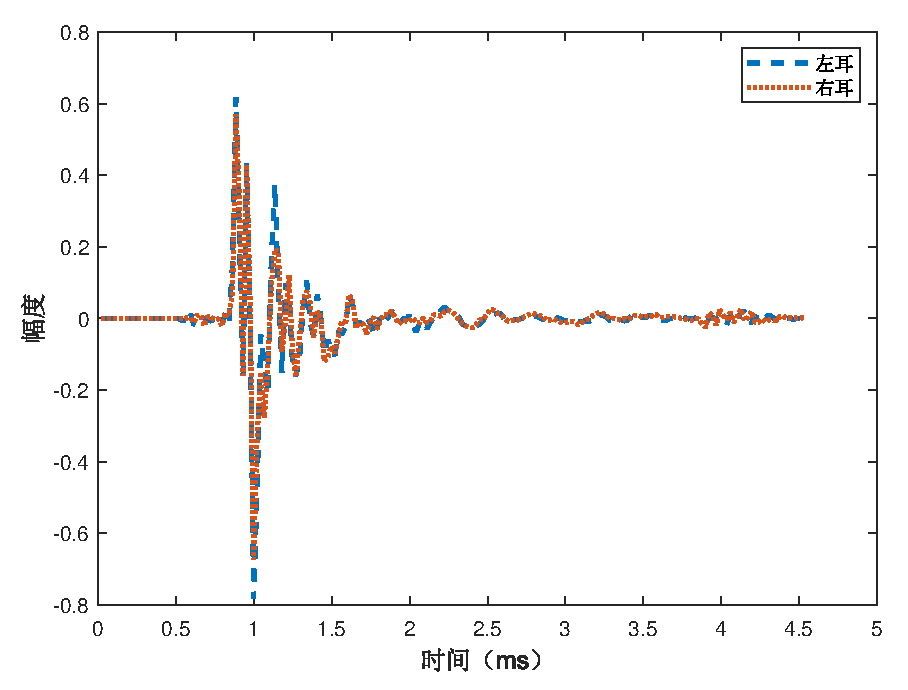
\includegraphics[width=0.48\textwidth]{figure/chapter3/0du_HRIR}}
\hfill
\subfigure[]{
\includegraphics[width=0.48\textwidth]{figure/chapter3/0du_HRTF}}
\caption{CIPIC~数据库中声源位于水平面且方向为~$0^{\circ}$~时的左右耳~HRIR~和~HRTF~数据:(a)~HRIR,(b)~HRTF}
\label{fig:CIPIC_0du}
\end{figure}

% 由于测量系统的力学和物理特性,所测量的HRTFs将不可避免地包含一定的噪声。为了避免噪声的影响,此处的结果展示采用~MESH2HRTF~数据库。


\subsection{HRTF~的球谐系数估计}\label{subsec.HRTF_coe}

% 突然想到一个问题,对于HRTF的分解求解,之前用的是空心球的公式,但是人头是不是应该用刚球? 但人头好像又不能看作是刚性球,刚性球是有条件的,人头的散射反射又不能忽略。  因此不能看作是刚球,所以还是应该使用空心球的公式进行计算。

由于~CIPIC~数据库采用双耳极坐标系,与球谐函数的角度定义不一致,所以在~HRTF~球谐分解之前,需要对~CIPIC~数据库的角度进行转换。
在转换过程中也可以借助~CIPIC~数据库的~SOFA~格式数据,在~SOFA~格式中,角度定义与图~\ref{fig:harmonics_theta_phi_definition}~类似,仅在俯仰角~$\theta$~的定义上不同,其俯仰角为方向矢量与水平面的夹角。

同时为了方便分析,本文对方位角重新定义。 图~\ref{fig:harmonics_theta_phi_definition}~中的俯仰角~$\theta$~为方向矢量与~$z$~正轴的夹角,$\theta=0^{\circ}~,~90^{\circ}~,180^{\circ}~$~分别表示正上方、水平面和正上方,其中水平面是指由原点指向正前方和正右(或左)方的两矢量决定的平面。方位角~$\phi$~为方向矢量在水平面的投影与中垂面的夹角,在水平面上,$\phi=0^ {\circ}~,~90^{\circ}~,180^{\circ}~,270^{\circ}~$~分别表示正前、正左、正后和正右方。
调整后,俯仰角不变,在水平面上,方位角~$\phi=0^{\circ}~,~90^{\circ}~,180^{\circ}~,270^{\circ}~$~分别表示正前、正右、正后和正左方。详见表格~\ref{tab.angel_transform}。

\begin{table}[H]
\centering
\caption{转换前后的角度定义}
\begin{tabular}{|c|c|c|c|}
\hline
   & SOFA~格式角度定义 & 球谐函数角度定义 & 最终角度定义 \\
\hline
俯仰角~$\theta$ & 矢量与水平面的夹角 &  矢量与~$x$~正轴的夹角& 矢量与~$x$~正轴的夹角  \\
 & $-90^{\circ} \leq \theta \leq 90^{\circ} $ & $0 \leq \theta \leq 180^{\circ} $ & $0 \leq \theta \leq 180^{\circ} $ \\
\hline
正上方 & $\theta = 90^{\circ}$ & $\theta = 0^{\circ}$ & $\theta = 0^{\circ}$ \\
水平面 & $\theta = 0^{\circ}$ & $\theta = 90^{\circ}$ & $\theta = 90^{\circ}$ \\
正下方 & $\theta = -90^{\circ}$ & $\theta = 180^{\circ}$ & $\theta = 180^{\circ}$ \\
\hline
正前方 & $\phi = 0^{\circ}$ & $\phi = 0^{\circ}$ & $\phi = 0^{\circ}$ \\
正右方 & $\phi = 270^{\circ}$ & $\phi = 270^{\circ}$ & $\phi = 90^{\circ}$ \\
正后方 & $\phi = 180^{\circ}$ & $\phi = 180^{\circ}$ & $\phi = 180^{\circ}$ \\
正左方 & $\phi = 90^{\circ}$ & $\phi = 90^{\circ}$ & $\phi = 270^{\circ}$ \\
\hline
\end{tabular}
\label{tab.angel_transform}
\end{table}

从~SOFA~格式角度定义到最终角度定义的转换公式为:
\begin{align}
\phi & = mod~\left( 360^{\circ}-\phi_{\text{SOFA}}, 360^{\circ} \right) \nonumber \\
\theta & =  90^{\circ} - \theta_{\text{SOFA}},
\end{align}
其中,$mod$~表示取余。

接下来对进行角度转换后的~HRTF~数据进行球谐分解。由~\ref{sec.SHdecomposition}~节可知,$P$~个方位的~HRTF~可以使用球谐函数进行分解:
\begin{equation}\label{HRTF_decomposition}
H_{\text{L,R}}(\theta_{p},\phi_{p},f)  = \sum_{n=0}^{N_{h}}\sum_{m=-n}^{n} \beta_{nm}^{L,R}(f)Y_{n}^{m}(\theta_{p},\phi_{p})
\end{equation}

球谐系数的求解方式~$\beta_{nm}^{L,R}(f)$~的方法与式~\eqref{eq.coeMat_random_sampling}~类似:
\begin{equation}
\bm{H}_{\text{L,R}} = \bm{Y} \bm{\beta_{nm}}^{\text{L,R}},
\end{equation}
其中,$\bm{Y}$~是大小为~$P \times (N_{h}+1)^2$~的矩阵,$\bm{H}_{\text{L,R}}$~和~$\bm{\beta_{nm}}^{\text{L,R}}$~是长度为~$P$~和~$(N_{h}+1)^2$~的列向量,
\begin{equation}
\bm{Y}=\left[
\begin{array}{ccccc}
Y_{0}^{0}\left(\theta_{1}, \phi_{1}\right) & \cdots & Y_{n}^{m}\left(\theta_{1}, \phi_{1}\right) & \cdots & Y_{N_{h}}^{N_{h}}\left(\theta_{1}, \phi_{1}\right) \\
Y_{0}^{0}\left(\theta_{2}, \phi_{2}\right) & \cdots & Y_{n}^{m}\left(\theta_{2}, \phi_{2}\right) & \cdots & Y_{N_{h}}^{N_{h}}\left(\theta_{2}, \phi_{2}\right) \\
\vdots & \ddots & \vdots & \vdots  & \vdots \\
Y_{0}^{0}\left(\theta_{P}, \phi_{P}\right) & \cdots & Y_{n}^{m}\left(\theta_{P}, \phi_{P}\right) & \cdots & Y_{N_{h}}^{N_{h}}\left(\theta_{P}, \phi_{P}\right)
\end{array}\right],
\end{equation}
\begin{equation}
\bm{H}_{\text{L,R}} = [H_{\text{L,R}}(\theta_{1},\phi_{1},f),~H_{\text{L,R}}(\theta_{2},\phi_{2},f)~,~\cdots~,~H_{\text{L,R}}(\theta_{P},\phi_{P},f)]^{T},
\end{equation}
\begin{equation}
\bm{\beta_{nm}}^{\text{L,R}} = [\beta_{0,0}^{\text{L,R}}~,\cdots,~\beta_{n,m}^{\text{L,R}}~,~\cdots~,~\beta_{N_{h},N_{h}}^{\text{L,R}}]^{T}.
\end{equation}


对于~HRTF~数据库来说,球面采样一般较为密集,假设采样点总数满足~$P>(N_{h}+1)^2$~,因此可以采用式~\eqref{eq.HRTF_Pinv}~进行球谐分量的求解。
\begin{equation}\label{eq.HRTF_Pinv}
\bm{\beta_{nm}}^{\text{L,R}} = \bm{Y}^{\dagger}\bm{H_{\text{L,R}}}= (\bm{Y}^{H}\bm{Y})^{-1}\bm{Y}^{H}\bm{H_{\text{L,R}}}.
\end{equation}

球谐分量~$\bm{\beta_{nm}}^{\text{L,R}}$~也可以用于重建任意方位的~HRTF~,又称为~HRTF~插值。任意方向~$(\theta,\phi)$~的~HRTF~的表达式为:
\begin{equation}
\hat{H}_{\text{L,R}}(\theta,\phi,f) = \bm{y} \bm{\beta_{nm}}^{\text{L,R}}.
\end{equation}

其中,$\bm{y} = \left[ Y_{0}^{0}(\theta,\phi)~,~ \cdots~,~Y_{n}^{m}(\theta,\phi)~,~\cdots~,~ Y_{N_{h}}^{N_{h}}(\theta,\phi)\right]$~为重建方位~ $(\theta,\phi)$~对应的球谐函数向量。

\section{HRTF~预处理}\label{sec.HRTF_pre}

从~\ref{sec.SHdecomposition}~节可知,直接使用低阶截断的~HRTF~分量进行双耳渲染会带来许多问题,因此需要引入~HRTF~预处理方法进行改进。一些~HRTF~预处理方法通过寻找对~HRTF~更为紧凑的表示,使大部分能量集中在球谐分解的低阶分量上。本节将对~HRTF~的预处理方法之一~——~双耳对准加以介绍,并且通过实验验证了该方法的有效性。




\subsection{预处理方法}

为了降低~HRTF~的低阶球谐表示所引起的误差,建议引入预处理来降低~HRTF~的有效球谐阶数。
对于式~\eqref{HRTF_decomposition}~中对~HRTF~的球谐分解,其高阶球谐分量主要是由高频处快速的相位变化导致的。并且研究表明,去除或者改变高频处的双耳相位差~(interaural phase difference~,~IPD)~在感知上无关紧要~\tcite{2015Efficient}。在此基础上,对~HRTF~进行相位修正的预处理方法被用于~HRTF~低阶球谐分解的扩展工作。
例如,对高频应用时间对准,即通过减去高频部分的线性相位部分来实现~IPD~均衡~\tcite{2018Binaural}\tcite{2018comparison},可以降低~HRTF~数据库的空间复杂度,从而降低所需的球谐分解阶次。


知觉研究表明,听觉系统在判断声源方位时所使用的声学信息是有选择性的,在自由场情况下,人耳听觉系统对单一声源进行定位时,主要定位因素双耳时间差~ITD~和双耳声级差~ILD~随着频率的作用范围如下所示:
\begin{compactitem}
\item 在频率小于~1.5~kHz~的情况下,双耳时间差~ITD~是方向定位的主要因素;
\item 在频率为~1.5~kHz~到~4~kHz~的情况下,双耳时间差~ITD~和双耳声级差~ILD~对方向定位共同起作用;
\item 在频率大于~4~kHz~到~5~kHz~的情况下,双耳声级差~ILD~是方向定位的主要因素。
\end{compactitem}


基于高频处~HRTF~的幅度部分对定位的感知起决定作用这一事实,在本研究中,采用了与之前相同的处理方法,对高频相位加以修正。主要关注对高频处~HRTF~幅度的近似,而相位从临界频率开始加以改变。

加以相位对准的头相关传递函数~
$H_{\text{L,R}}^{a}(\theta,\phi,f)$~可表示为:
\begin{equation}\label{eq.HRTF_pre}
H_{\text{L,R}}^{a}(\theta,\phi,f) =
\begin{cases}
 H_{\text{L,R}}(\theta,\phi,f)  ,  & f<f_{c} \\
 H_{\text{L,R}}(\theta,\phi,f) e^{i\zeta} , & f \geq f_{c},
\end{cases}
\end{equation}
其中,$f_{c}$~为临界频率,一般选取~1.5~kHz。对于给定的频率,$\zeta$~的表达式为:
\begin{align}
\zeta & = \angle \left(~ [ H_{\text{L,R}}(\theta,\phi,f)]^{*} H_{\text{L,R}}(\theta,\phi,f_{c})~\right) \nonumber \\
& = \angle \left(~ H_{\text{L,R}}(\theta,\phi,f_{c}) ~\right) - \angle \left(~ H_{\text{L,R}}(\theta,\phi,f) ~\right),
\end{align}
其中,$\angle(\cdot)$~表示取一个复数的相位信息。

上述公式给出了直接从~HRTF~数据中获取相位差的方法,也可以根据声源方位和人头尺寸等参数获取,如下所示:
\begin{equation}\label{eq.time_align}
\zeta = 2\pi (f_{c} - f) \tau_{p}^{\text{L,R}},
\end{equation}
其中,$\tau_{p}^{\text{L,R}}$~为声源位于~$(\theta_{p},\phi_{p})$~位置处对应的时间偏移,即头中心和耳朵之间的时间差。

假设为远场条件,此时声源信号可以看作平面波,因此$\tau_{p}^{\text{L,R}}$~的计算公式为:
\begin{equation}
\tau_{p}^{r}=\cos \left(\theta_{p}\right) \sin \left(\phi_{p}\right) a/c, \quad \tau_{p}^{l}=-\tau_{p}^{r}
\end{equation}

使用式~\eqref{eq.time_align}~通过时间差计算相位差从而对~HRTF~进行对准的方法一般被称为时间对准。时间对准的~HRTF~和相位对准的~HRTF~方法的原理基本一致,核心思想是将原有的~HRTF~中使用自由场下头中心处的声压对双耳声压进行归一化转换为使用双耳所在位置的声压对双耳声压进行归一化,此处方法已被证明是一种有效降低~HRTF~SH~阶次的稳健方法,有很多工作基于此进行~\tcite{2018Binaural}\tcite{2019Efficient}\tcite{ben2020binaural}。

和直接使用最小二乘方法求解头相关传递函数的球谐分量相比,该预处理方法一方面准确地表示头相关传递函数的幅度谱,并有效降低了头相关传递函数的分解阶次。

请注意,与其他以前建议的有效的~HRTF~表示方法不同,该相位校正过程是可逆的,这意味着从原始~HRTF~到经过对准的~HRTF~再到原始~HRTF~不会丢失任何信息。

\newpage
\subsection{实验结果与分析}\label{sec.Pre_result}

为了衡量~HRTF~预处理算法对球谐分解所带来的影响,定义~HRTF~球谐分解分量在~$n$~阶下的能量~$E_{\text{L,R}}(f,n)$~和所有阶次下的累积能量~$E_{\text{L,R}}^{C}(f,n)$~为:
\begin{equation}
E_{\text{L,R}}(f,n) = \sum_{m=-n}^{n} | \beta_{nm}^{\text{L,R}}(f) |^{2},
\end{equation}
\begin{equation}
E_{\text{L,R}}^{C}(f,n) = \sum_{n=0}^{N_{h}} \sum_{m=-n}^{n} | \beta_{nm}^{\text{L,R}}(f) |^{2}.
\end{equation}

为了避免测试环境对预处理前后阶次变化的影响,本节采用消声室环境下使用~Neumann~KU-100~在~2702~点球面列别捷夫采样下的远场数据库~\tcite{Benjamin2013A}。在计算过程中,对能量进行归一化,并对归一化能量取对数~$10\text{lg}\left( E_{\text{L,R}}(f,n)\right)$。预处理前后的球谐分量的能量分布如图~\ref{fig:pre_after}~所示,图中黑色实线表示有效球谐分解阶次,即前~$N$~阶球谐分量包含了~HRTF~$99\%$~的能量。

\begin{figure}[H]
\centering
\subfigure[]{
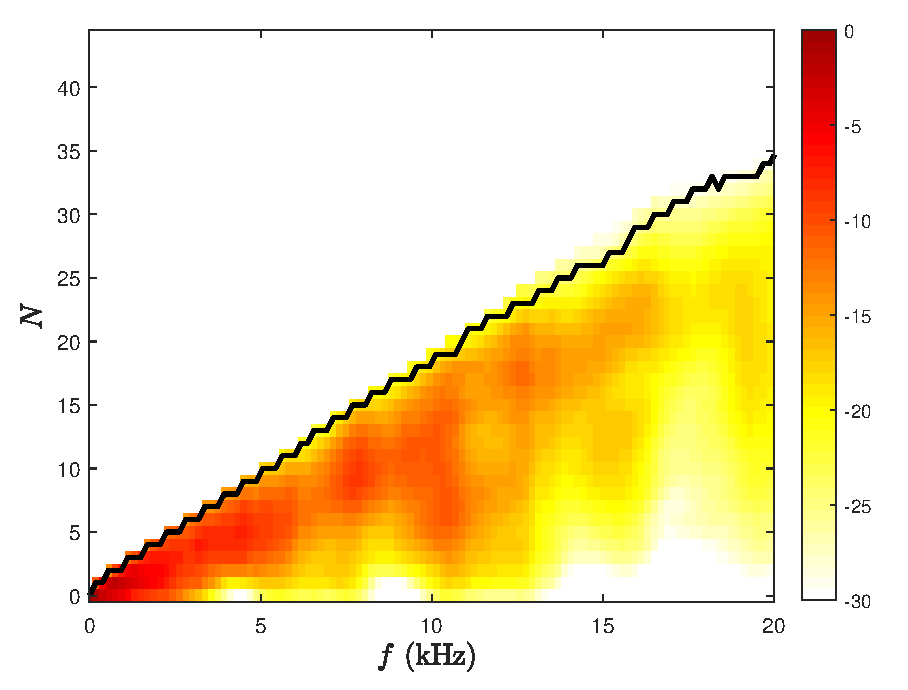
\includegraphics[width=0.48\textwidth]{figure/chapter3/nopre}}
\hfill
\subfigure[]{
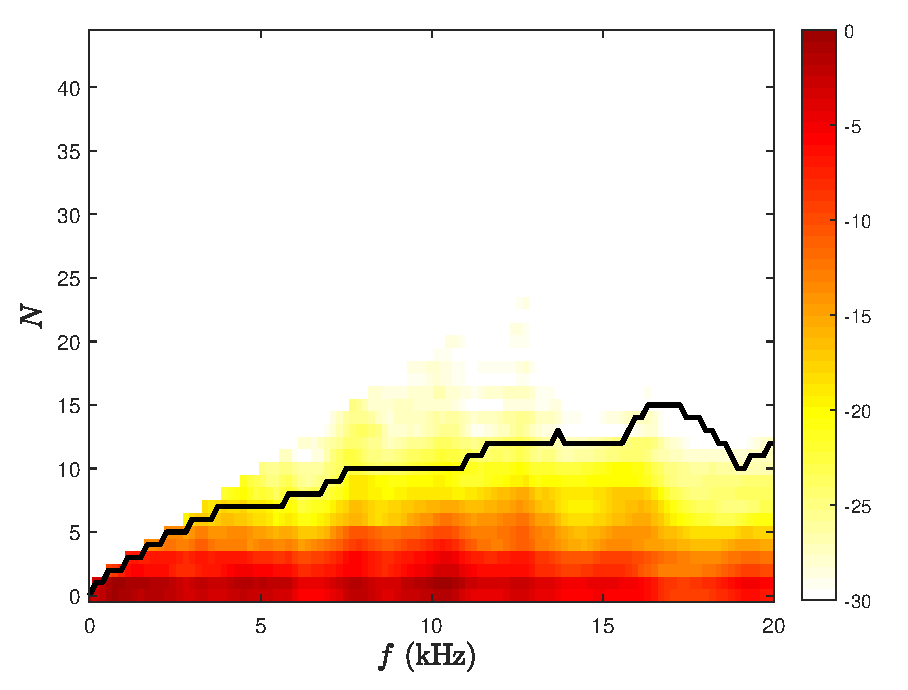
\includegraphics[width=0.48\textwidth]{figure/chapter3/pre}}
\caption{预处理前后~HRTF~的能量分布:~(a)预处理前,(b)预处理后}
\label{fig:pre_after}
\end{figure}


从图~\ref{fig:pre_after}~可以看出:
\begin{inparaenum}[(1)]

\item 未引入预处理时,HRTF~球谐分解所需阶次较大,并且随着频率的增加,球谐分解阶次逐渐增加;

\item 对头相关传递函数加以预处理后,HRTF~球谐分解所需阶次较小,并且随着频率的增加,球谐分解阶次趋于稳定;

\item 与频率相关的双耳对准预处理算法可以有效降低~HRTF~的分解阶次,由原来的~34~阶降低至~15~阶。

\end{inparaenum}

\section{本章小结}

本章对基于球谐分解的双耳渲染进行了详细的理论推导,并针对其存在的不匹配问题,对~HRTF~进行预处理。 首先,对声场的球谐系数估计进行推导,并且针对空心球和刚性球两种情况给出了不同的计算方法。其次对~HRTF~数据库、HRTF~的球谐系数估计以及对~HRTF~数据库进行球谐分解的前提~——~角度转换进行了详细介绍。并引入~HRTF~预处理方法,以降低~HRTF~的球谐分解阶次和提升双耳感知。实验结果表明,与频率相关的双耳对准预处理算法可以有效降低~HRTF~的分解阶次。


\chapter{基于声场扩阶的双耳渲染算法 }\label{chapter.AddWindow}

由于实际情况的限制,基于球谐分解的双耳渲染算法在声场和~HRTF~之间存在不匹配问题,第~\ref{chapter.HRTF}~章中对~HRTF~进行相位对准预处理,以降低~HRTF~的球谐分解阶次。声场在算法中和~HRTF~有着同等重要的地位, 但是目前的算法均集中于~HRTF~预处理。本章将从声场角度出发,提出一种新的声场扩阶算法,以提升声场的球谐分解阶次。首先对信号模型进行介绍,其次对声场扩阶算法的原理进行详细介绍,即通过对原始录制声场进行空域加窗,以实现对录制声场分解阶次的提升,接下来对本文采用的空域窗函数加以介绍。并且将声场扩阶方法与~HRTF~预处理方法相结合,给出整体算法框图,共同解决目前双耳渲染中存在的问题。

\section{信号模型}\label{sec.modelAndMusic}
% 可以加入: 即使同时存在两个语音信息,在大多数时频点也只有一个声源。参见test或者球阵定位的相关文章。

考虑位于远场的一个声源信号和~$Q$~个麦克风,将麦克风在某个时频点上的接收信号建模为:
\begin{equation}\label{eq.model}
\bm{S} = \bm{S}_{p} + \bm{S}_{d},
\end{equation}
其中,第一项~$\bm{S}_{p}$~表示平面波,与声源的方位相关。其中,声源方位可以是直达波,也可以是早期反射,描述为在该时频点上能量较大的信号。第二项~$\bm{S}_{d}$~表示扩散声场(diffuse filed),由来自许多方向的不相关的平面波组成。第一项和第二项分别表示声源分量和环境分量。

该模型假设来源于语音信号的稀疏性。对于语音信号来说,常采用短时傅里叶变换(Short Time Fourier Transform,STFT),其在时频域上具有稀疏性,语音能量不仅集中在少数时间帧上,更集中在少量的时频单元上。

其中,第一项~$\bm{S}_{p}$~对应的声源方位可以通过许多方法进行获取,估计声源的到达方向(direction of arrival,DOA)一直是人们关注的领域。基于波束形成、最大似然以及子空间方法等各种~DOA~估计方法之前已被广泛研究,并且在球形麦克风阵列上加以扩展~\tcite{2012Localization},接下来将简单介绍。

MUSIC~方法是非常经典的子空间~DOA~方法,其算法简单、高空间分辨率高,是目前比较流行的~DOA~估计算法之一,基于球形麦克风阵列的~MUSIC~方法可以在空域和球谐域上进行,本文主要关注基于球阵的球谐域~MUSIC~算法。对球形麦克风阵列的采集信号进行~SH~变换转换到球谐域的好处是,与传统的空域~MUSIC~算法相比,球谐域~MUSIC~算法通过解耦去除球谐域中与频率相关的分量,其阵列流形矩阵与频率无关,独立于阵列设置,且计算简单~\tcite{2012Localization}。

假设有~$J$~个幅度为~$s_{j}(f)$,来波方向为~$(\theta_{j},\phi_{j})$~的平面波,由公式~\eqref{SMic_pressure}~可得,第~$q$~个麦克风的接收信号和其球谐分解系数分别为:
\begin{equation}
   S(r,\theta_q,\phi_q,f)=
   \sum _{n=0}^{\infty}\sum _{m=-n}^{n}\sum_{j=1}^{J} s_{j}(f) b_n(kr) Y_n ^{m}(\theta_q,\phi_q) [Y_n ^{m}(\theta_j,\phi_j)]^{*},
\end{equation}
和
\begin{equation}\label{eq.Snm_Jplane}
   S_n ^m(r,f) =
    b_n(kr) \sum_{j=1}^{J} s_{j}(f) [Y_n ^{m}(\theta_j,\phi_j)]^{*}.
\end{equation}

定义~$s_n ^m(f) = S_n ^m(r,f) / b_n(kr)$~,式~\eqref{eq.Snm_Jplane}~可写为:
\begin{equation}
   s_n^m(f) =
    \sum_{j=1}^{J} s_{j}(f) [Y_n ^{m}(\theta_j,\phi_j)]^{*},
\end{equation}
其矩阵形式为:
\begin{equation}
   \bm{s_n^m} =
    \bm{Y^{H} s},
\end{equation}
其中,$\bm{s_n^m}$~是一个长度为~$(N_{s}+1)^2$~的向量:
\begin{equation}
\bm{s_n^m} = [~s_{0}^{0}(f)~,~s_{1}^{-1}(f)~,~s_{1}^{0}(f)~,~s_{1}^{1}(f)~,~\cdots~,~~s_{N_{s}}^{N_{s}}(f)]^{T},
\end{equation}
$\bm{s}$~是一个长度为~$J$~的平面波幅度向量:
\begin{equation}
\bm{s} = [~s_{1}(f)~,~s_{2}(f)~,~\cdots~,~s_{J}(f)~]^{T},
\end{equation}
$\bm{Y}$~是一个~$J\times(N_{s}+1)^2$~的球谐域流形矩阵,其中第~$j$~行为声源位于~$(\theta_{j},\phi_{j})$~方位处的球谐域流行向量,表示为:
\begin{equation}\label{eq.y}
\mathbf{y}(\theta_{j},\phi_{j}) = [~Y_{0}^{0}(\theta_{j},\phi_{j})~,~\cdots~,~Y_{n}^{m}(\theta_{j},\phi_{j})~,~Y_{N_{s}}^{N_{s}}(\theta_{j},\phi_{j})~]
\end{equation}
由式~\eqref{eq.y}~可知,球谐域~MUSIC~算法的阵列流形矩阵与频率无关,且独立于阵列设置,即与麦克风所在位置无关。

相关谱矩阵可以由下式得到:
\begin{equation}
\hat{\mathbf{S}}=\bm{s_n^m} [\bm{s_n^m}]^{H}
\end{equation}
则~MUSIC~谱函数可以表示为:
\begin{equation}
P_{MU}(\theta,\phi)=\frac{1}{\mathbf{y}(\theta,\phi) \mathbf{E}_{N_{s}} \mathbf{E}_{N_{s}}^{H} \mathbf{y}^{H}(\theta,\phi)},
\end{equation}
其中,矩阵~$\mathbf{E}_{N_{s}}$~是噪声子空间,每一列对应一个噪声特征向量,是矩阵~$\hat{\mathbf{S}}$~最小的~$(N_{s}+1)^2-J $~个特征值对应的特征向量,这些特征向量可以通过对矩阵~$\hat{\mathbf{S}}$~进行特征值分解获得。令~$(\theta,\phi)$~在空间中变化,搜索~$P_{MU}(\theta,\phi)$~的~$J$~个峰值,对应的角度即为平面波来波方向的估计值。

在本文中,如式~\eqref{eq.model}~所示,假设每一个时频点只存在一个平面波,此时~$J=1$,噪声子空间中特征向量的数目为~$(N_{s}+1)^2-1 $。

在此对球贝塞尔函数的零点问题(如图~\ref{fig:bn}~所示)给定位算法带来的影响加以讨论。如上述定义~$s_n ^m(f) = S_n ^m(r,f) / b_n(kr)$~所示,使用球谐域~MUSIC~算法进行定位时需要对所获取的球谐分量~$S_n ^m(r,f)$~除以~$b_{n}(kr)$。对于单个空心球来说,即需要除以~$j_{n}(kr)$,这将导致~$s_n ^m(f)$~为一极大值,带来很大的定位误差。对于刚性球来说,则可以很好地避免这个问题。


\section{声场扩阶原理}

本节将对所提出的声场扩阶原理进行详细介绍,首先给出了有界线性算子及其在球谐域的表示形式,以此为基础对空域加窗算子在球谐域上的表示进行了详细推导,得到加窗后信号的球谐系数表达式,并且对空域加窗带来的声场扩阶现象加以分析。

\subsection{有界线性算子}
对于一个在~$L^{2}(\mathbb{S}^{2})$~空间的有界线性算子~$\mathcal{B}$~\tcite{Hilbert},将~$S(\theta,\phi)$~映射到~$G(\theta,\phi)$(简便起见,麦克风位置~$r$~和频率~$f$~省略不写),记作:
\begin{equation}
G(\theta,\phi) = \left(\mathcal{B} S\right) (\theta,\phi)
\end{equation}
也可以简记为~$G = \mathcal{B} S $。在大多数情况下,$\mathcal{B}$~用于表示一个通用的有界操作符,或者在特定有界运算符的表示中用作统称。

在可分离的希尔伯特空间,对于一个给定的完备正交序列~$\{\psi\}_{n=1}^{\infty}$,任意一个有界线性算子~$\mathcal{B}$~可以使用一个无限矩阵~$\mathbf{B}^{(\psi)}$~等价表示。矩阵在第~$n$~行~$m$~列的元素~$b_{n,m}^{(\psi)}$~表示沿着~$\psi_{m}$~方向的输入与经过该有界线性算子~$\mathcal{B}$~后沿着~$\psi_{n}$~方向的输出之间的关系。

由于~$L^{2}(\mathbb{S}^{2})$~空间是可分离的,并且球谐函数是一个完备正交序列。因此,可以结合球谐分解得到有界线性算子在球谐域的表示形式。映射前后的信号可表示为:
\begin{equation}\label{S_pq_infty}
S(\theta,\phi) = \sum_{n=0}^{\infty}\sum_{m=-n}^{n} S_{n}^{m} Y_{n}^{m}(\theta,\phi).
\end{equation}
\begin{equation}\label{G_lm_infty}
G(\theta,\phi) =  \sum_{p=0}^{\infty} \sum_{q=-p}^{p} G_{p}^{q} Y_{p}^{q}(\theta,\phi).
\end{equation}

我们几乎只用球谐函数作为完备正交序列,因此可以去掉对基函数上标~$\psi$~的依赖性,简单地把~$\mathbf{B}^{(\psi)}$~写成~$\mathbf{B}$~的形式。

此时,算子~$\mathcal{B}$~可以用无限矩阵~$\mathbf{B}$~表示,其矩阵元素~$b_{p,n}^{q,m}$~表示的是以~$Y_{n}^{m}$~为输入,
经过算子~$\mathcal{B}$~后输出信号在~$Y_{p}^{q}$~方向的分量,表示为:
\begin{equation}\label{eq.b_lmpq}
b_{p,n}^{q,m} = \left< \mathcal{B}Y_{n}^{m},Y_{p}^{q} \right>,
\end{equation}
其中,$\left< \cdot \right>$~表示内积,式~\eqref{eq.b_lmpq}~可进一步表示为:

\begin{equation}
b_{p,n}^{q,m} = \int_{0}^{2\pi}\int _{0}^{\pi} B(\theta,\phi)Y_{n}^{m}(\theta,\phi) \left[Y_{p}^{q}(\theta,\phi) \right]^{*}\sin\theta d\theta d\phi
\end{equation}

在式~\eqref{eq.b_lmpq}~中,一对~$m$~和~$n$~对应矩阵~$\mathbf{B}$~的一列,即第~$n^2+n+m+1$~列,一对~$p$~和~$q$~对应矩阵~$\mathbf{B}$~的一行,即第~$p^2+p+q+1$~行,算子矩阵~$\mathbf{B}$~如下所示:

\begin{align}
\mathbf{B} & =\left[
\begin{array}{cccc}
b_{0,0} & b_{0,1} & b_{0,2} & \cdots  \\
b_{1,0} & b_{1,1} & b_{1,2} & \cdots  \\
b_{2,0} & b_{2,1} & b_{2,2} & \cdots   \\
\vdots & \vdots &  \vdots  & \ddots
\end{array}\right]
= \left[
\begin{array}{c|ccc|cc}
b_{0,0}^{0,0} & b_{0,1}^{0,-1} & b_{0,1}^{0,0} & b_{0,1}^{0,1} & b_{0,2}^{0,-2} & \cdots  \\
\hline
b_{1,0}^{-1,0} & b_{1,1}^{-1,-1} & b_{1,1}^{-1,0} & b_{1,1}^{-1,1} & b_{1,2}^{-1,-2} & \cdots  \\
b_{1,0}^{0,0} & b_{1,1}^{0,-1} & b_{1,1}^{0,0} & b_{1,1}^{0,1} & b_{1,2}^{0,-2} & \cdots  \\
b_{1,0}^{1,0} & b_{1,1}^{1,-1} & b_{1,1}^{1,0} & b_{1,1}^{1,1} & b_{1,2}^{1,-2} & \cdots  \\
\hline
b_{2,0}^{-2,0} & b_{2,1}^{-2,-1} & b_{2,1}^{-2,0} & b_{2,1}^{-2,1} & b_{2,2}^{-2,-2} & \cdots  \\
\vdots & \vdots &  \vdots  & \vdots &  \vdots & \ddots
\end{array}\right].
\end{align}

因此有界算子~$\mathcal{B}$~将~$S\in L^{2}\left(\mathbb{S}^{2}\right)$~的球谐系数~$S_ {n}^{m}=\left< S, Y_{n}^{m}\right> $~映射到~$G \in L^{2}\left(\mathbb{S}^{2}\right)$~的球谐系数~$G_{p}^{q} = \left<G,Y_{p}^{q}\right> = \left<\mathcal{B}S,Y_{p}^{q}\right>$,则~$G_{p}^{q} $~和~$G(\theta,\phi)$~可以表示为:
\begin{equation}\label{eq.G_lm}
G_{p}^{q}  = \sum_{n=0}^{\infty}\sum_{m=-n}^{n} S_{n}^{m} b_{p,n}^{q,m}
\end{equation}
\begin{equation}
G(\theta,\phi) = \sum_{p=0}^{\infty} \sum_{q=-p}^{p}\sum_{n=0}^{\infty}\sum_{m=-n}^{n} S_{n}^{m} b_{p,n}^{q,m} Y_{p}^{q}(\theta,\phi)
\end{equation}

对于复合算子~$\mathcal{P = B \cdot D }$,其算子矩阵可以简单地由各个算子的算子矩阵给出,其算子矩阵元素可表示为:
\begin{equation}
p_{p,s}^{q,t} = \sum_{n=0}^{\infty} \sum_{m=-n}^{m} b_{p,n}^{q,m} d_{n,s}^{m,t},
\end{equation}
其中,$p_{p,s}^{q,t}$、$b_{p,n}^{q,m}$~和~$d_{n,s}^{m,t}$~分别为~$\mathcal{P}$、$\mathcal{B}$~和~$\mathcal{D}$~的算子矩阵元素。

\subsection{空域加窗}\label{subsec.Addwindow}
在空间域使用窗函数对一个信号进行掩蔽,即将感兴趣的信号~$S(\theta,\phi)$~与设计合理的窗函数~$h(\theta,\phi)$~在空间域上逐点相乘。将空域加窗对应的空间掩蔽算子记为~$\mathcal{B}_{h}$~,则加窗后信号在空间域的表达式为:
\begin{equation}
\left( \mathcal{B}_{h} S\right)(\theta,\phi) = h(\theta,\phi)S(\theta,\phi),
\end{equation}
其中,$h(\theta,\phi)$~为空域窗函数。

空间掩蔽算子~$\mathcal{B}_{h}$~对应的算子矩阵元素为:
\begin{equation}
b_{p,n}^{q,m} = \int_{0}^{2\pi}\int _{0}^{\pi} h(\theta,\phi)Y_{n}^{m}(\theta,\phi) \left[Y_{p}^{q}(\theta,\phi) \right]^{*}\sin\theta d\theta d\phi.
\end{equation}


与式~\eqref{S_pq_infty}~和~\eqref{G_lm_infty}~类似,对窗函数~$h(\theta,\phi)$~进行球谐分解:
\begin{equation}\label{h_st_infty}
h(\theta,\phi) = \sum_{s=0}^{\infty} \sum_{t=-s}^{s} h_{s}^{t} Y_{s}^{t}(\theta,\phi)
\end{equation}
其中,$h_{s}^{t}$~为窗函数的球谐系数。

因此式~\eqref{eq.G_lm}~可以表示为:
\begin{align}
G_{p}^{q} &= \sum_{n=0}^{\infty}\sum_{m=-n}^{n} S_{n}^{m} b_{p,n}^{q,m} \nonumber \\
& = \sum_{n=0}^{\infty}\sum_{m=-n}^{n}  S_{n}^{m}\int_{0}^{2\pi}\int _{0}^{\pi} h(\theta,\phi)Y_{n}^{m}(\theta,\phi) \left[Y_{p}^{q}(\theta,\phi) \right]^{*}\sin\theta d\theta d\phi \nonumber \\
& = \sum_{n=0}^{\infty}\sum_{m=-n}^{n}  S_{n}^{m}\int_{0}^{2\pi}\int _{0}^{\pi} \sum_{s=0}^{\infty} \sum_{t=-s}^{s} h_{s}^{t} Y_{s}^{t}(\theta,\phi) Y_{n}^{m}(\theta,\phi) \left[Y_{p}^{q}(\theta,\phi) \right]^{*}\sin\theta d\theta d\phi \nonumber \\
& = \sum_{n=0}^{\infty}\sum_{m=-n}^{n} S_{n}^{m}\sum_{s=0}^{\infty} \sum_{t=-s}^{s} h_{s}^{t}\int_{0}^{2\pi}\int _{0}^{\pi}Y_{s}^{t}(\theta,\phi) Y_{n}^{m}(\theta,\phi) \left[Y_{p}^{q}(\theta,\phi) \right]^{*}\sin\theta d\theta d\phi
\end{align}

为上式的积分定义一个简记法:
\begin{equation}\label{y_stlmpq}
y(s,t;n,m;p,q) \triangleq \int_{0}^{2\pi}\int _{0}^{\pi}Y_{s}^{t}(\theta,\phi) Y_{n}^{m}(\theta,\phi) \left[Y_{p}^{q}(\theta,\phi) \right]^{*}\sin\theta d\theta d\phi,
\end{equation}
此时,空间掩蔽算子~$\mathcal{B}_{h}$~对应的算子矩阵元素为:
\begin{equation}
b_{p,n}^{q,m} = \sum_{s=0}^{\infty} \sum_{t=-s}^{s} h_{s}^{t} y(s,t;n,m;p,q).
\end{equation}
加窗后信号的球谐分解系数可以简洁表示为:
\begin{equation}\label{eq.AddWindow_infty}
G_{p}^{q} = \sum_{n=0}^{\infty} \sum_{m=-n}^{n} S_{n}^{m}\sum_{s=0}^{\infty} \sum_{t=-s}^{s} h_{s}^{t}y(s,t;n,m;p,q).
\end{equation}

在量子力学中经常出现包含三个球谐函数的积分,可以用~Wigner~$3j$~符号表示~\tcite{Wigner_3j},式~\eqref{y_stlmpq}~可表示为:
\begin{equation}
y(s,t;n,m;p,q) = (-1)^{q} \sqrt{\frac{(2 s+1)(2 n+1)(2 p+1)}{4 \pi}}\left(\begin{array}{ccc}
s & n & p \\
0 & 0 & 0
\end{array}\right)\left(\begin{array}{ccc}
s & n & p \\
t & m & -q
\end{array}\right),
\end{equation}
其中,后两项不是矩阵,而是~Wigner~$3j$~符号,将在下文对该符号的定义和计算公式进行简单介绍。


Wigner~$3j$~符号是~Wigner~在文献~\cite{Wigner_3j}~中定义的~$3j$~符号,定义为:
\begin{equation}
\left(\begin{array}{ccc}
j_{1} & j_{2} & j_{3} \\
m_{1} & m_{2} & m_{3}
\end{array}\right) \triangleq \frac{(-1)^{j_{1}-j_{2}-m_{3}}}{\sqrt{2 j_{3}+1}} s_{j_{3}, m_{1}, m_{2}}^{j_{1}, j_{2}} \delta_{m_{1}+m_{2}+m_{3}, 0} ,
\end{equation}
其中~$s_{j 3, m_{1}, m_{2}}^{j_{1}, j_{2}}$~的表达式为:
\begin{align*}
s_{j_{3}, m_{1}, m_{2}}^{j_{1}, j_{2}} &=
\frac{\sqrt{\left(j_{3}+j_{1}-j_{2}\right) !\left(j_{3}-j_{1}+j_{2}\right) !\left(j_{1}+j_{2}-j_{3}\right) !\left(j_{3}-m_{3}\right) !\left(j_{3}+m_{3}\right) !}}{\sqrt{\left(j_{1}+j_{2}+j_{3}+1\right) !\left(j_{1}-m_{1}\right) !\left(j_{1}+m_{1}\right) !\left(j_{2}-m_{2}\right) !\left(j_{2}+m_{2}\right) !}}
\end{align*}
\begin{align*}
&  \times \sum_{t} \frac{(-1)^{t+j_{2}+m_{2}} \sqrt{2 j_{3}+1}\left(j_{3}+j_{2}+m_{1}-t\right) !\left(j_{1}-m_{1}+t\right) !}{\left(j_{3}-j_{1}+j_{2}-t\right) !\left(j_{3}-m_{3}-t\right) !(t) !\left(j_{1}-j_{2}+m_{3}+t\right) !}
\end{align*}
在关于~$t$~的求和项中要求所有阶乘内的参数都是非负的。

必须同时满足以下条件,Wigner~$3j$~符号才不是非零值:
\begin{equation}\label{eigner_if}
\begin{split}
m_{1}+m_{2}+m_{3}  = 0 \\
|j_{2}-j_{3}|  \leq j_{1}  \leq j_{2}+j_{3} \\
|j_{1}-j_{3}|  \leq j_{2}  \leq j_{1}+j_{3} \\
|j_{1}-j_{2}|  \leq j_{3}  \leq j_{1}+j_{2} \\
|m_{k}| \leq j_{k}~~,k = 1,2,3
\end{split}
\end{equation}

定义和计算Wigner~$3j$~符号的方法还有很多,其中最广泛使用的是~Racah~公式~\tcite{messiah1961quantum}:
\begin{equation}
\begin{array}{l}
\left(\begin{array}{ccc}
j_{1} & j_{2} & j_{3} \\
m_{1} & m_{2} & m_{3}
\end{array}\right)
=(-1)^{j_{1}-j_{2}-m_{3}} \sqrt{\Delta\left(j_{1}, j_{2}, j_{3}\right)} \\
\times \sqrt{\left(j_{1}-m_{1}\right) !\left(j_{1}+m_{1}\right) !\left(j_{2}-m_{2}\right) !\left(j_{2}+m_{2}\right) !\left(j_{3}-m_{3}\right) !\left(j_{3}+m_{3}\right) !} \\
\end{array}
\end{equation}
\begin{equation*}
\times \sum_{t} \frac{(-1)^{t}}{(t) !\left(j_{1}+j_{2}-j_{3}-t\right) !\left(j_{1}-m_{1}-t\right) !\left(j_{2}+m_{2}-t\right) !\left(j_{3}-j_{2}+m_{1}+t\right) !\left(j_{3}-j_{1}-m_{2}+t\right) !}
\end{equation*}
\\
其中~$\Delta\left(j_{1}, j_{2}, j_{3}\right)$~的表达式为:
\begin{equation*}
\Delta\left(j_{1}, j_{2}, j_{3}\right)=\frac{\left(j_{1}+j_{2}-j_{3}\right) !\left(j_{1}-j_{2}+j_{3}\right) !\left(j_{2}-j_{1}+j_{3}\right) !}{\left(j_{1}+j_{2}+j_{3}+1\right) !}
\end{equation*}

\subsection{空域加窗后的声场阶次}\label{sec.Enlarge_order}

在实际情况中,需要对式~\eqref{S_pq_infty}\eqref{G_lm_infty}\eqref{h_st_infty}~进行截断处理,假设加窗前信号、加窗后信号和窗函数球谐分解的最高阶次分别为~$N_{s}$、$N_{g}$~和~$N_{h'}$,由式~\eqref{eq.AddWindow_N}~可知~$N_{g}$~是由~$N_{s}$~和~$N_{h'}$~共同决定的。
\begin{equation}\label{eq.AddWindow_N}
G_{p}^{q} = \sum_{n=0}^{N_{s}} \sum_{m=-n}^{n} S_{n}^{m}\sum_{s=0}^{N_{h'}} \sum_{t=-s}^{s} h_{s}^{t}y(s,t;n,m;p,q)~,~~~~ 0\leq p \leq N_{g}.
\end{equation}

对于轴对称问题,即窗函数沿水平角~$\phi$~为常数的特殊情况,$N_{s}$、$N_{g}$~和~$N_{h'}$~有显示关系式。此时~$h(\theta,\phi) =h(\theta)$,窗函数的球谐系数为:

\begin{align}\label{h_st_constant}
h_{s}^{t} & = \int_{0}^{2\pi}\int_{0}^{\pi} h(\theta) \left[Y_{s}^{t}(\theta,\phi) \right]^{*}\sin\theta d\theta d\phi \nonumber\\
& = 2\pi \delta_{t,0} \sqrt{\frac{2s+1}{4\pi}} \int_{0}^{\pi}h(\theta) P_{s}^{t}(\cos\theta)\sin\theta d\theta \nonumber\\
& = \sqrt{\frac{4\pi}{2s+1}}h_{s}\delta_{t,0}~,
\end{align}
其中,$h_{s}$~只与~$s$~有关,这个性质是通过求解~$\phi$~的积分得到的,将原始的二维积分简化为一维,关联勒让德函数退化为勒让德函数。在这种情况下,$h_{s}$~可表示为:

\begin{align}
h_{s} & = \frac{2s+1}{2}\int _{0}^{\pi}h(\theta)P_{s}(\cos\theta)\sin\theta d\theta \nonumber \\
h(\theta) & = \sum_{s=0}^{\infty} h_{s}P_{s}(\cos\theta)~,
\end{align}
其中,$P_{s}(\cdot)$~为~$s$~阶勒让德函数。

结合式~\eqref{h_st_constant}~和式~\eqref{eigner_if}~可知,只有当~$m = q$~且~$|p-s| \leq n \leq |p+s|$~时,$y(s,t;n,m;p,q)$~才为非零值。此时,式~\eqref{eq.AddWindow_N}~可表示为:
\begin{equation}\label{eq.AddWindow_constant}
\begin{aligned}
G_{p}^{q}=(-1)^{q} \sqrt{\frac{(2p+1)}{4 \pi}} \sum_{s=0}^{N_{h'}} \sum_{n=|p-s|}^{p+s} h_{s}^{0} & S_{n}^{q} \sqrt{(2 s+1)(2 n+1)} \\
& \times\left(\begin{array}{ccc}
s & n & p \\
0 & 0 & 0
\end{array}\right)\left(\begin{array}{ccc}
s & n & p \\
0 & q & -q
\end{array}\right)
\end{aligned}
\end{equation}
由式~\eqref{eq.AddWindow_constant}可知,对于~$p \leq N_{h'}$,加窗后信号的球谐系数~$G_{p}^{q}$~是原始信号球谐系数~$S_{n}^{q}$~在阶次~$0 \leq n \leq p+N_{h'}$~上的加权和,对于~$p \geq N_{h'}$,加窗后信号分量~$G_{p}^{q}$~是原始信号分量~$S_{n}^{q}$~在阶次~$\left|p -N_{h'} \right| \leq n \leq p + N_{h'}$~上的加权和。因此,加窗后信号的球谐系数是原始信号的频谱平滑,平滑的程度取决于窗的带宽和频谱响应的形状。
并且,加窗后信号的球谐分解阶次最高可达到~$N_{g}=N_{s}+N_{h'}$。


\section{空域窗函数}\label{sec.window}

如上节所示,通过对原始信号进行空域加窗可以实现声场扩阶,本节将对采用的窗函数加以介绍。

本文中采用~Von Mises Fisher~函数~\tcite{2009Spatial}\tcite{2007Smoothing}\tcite{2002Spatial}~作为三维空间的窗函数,其可以认为是多元高斯函数在球坐标系下的近似。
在~$p-1$~维球体~$\mathbb{S}^{~p-1}$~上,Von Mises Fisher~函数的表达式为:
\begin{equation}\label{eq.Von}
h(\Omega ; \mu, \kappa)=C_{p}(\kappa) \exp ^{\kappa \bm{\mu}^{T} \bm{\Omega}} \sin \theta
\end{equation}
其中,主瓣方向(对称轴方向)向量~$\bm{\mu}$~是一个单位向量,即~$\|\bm{\mu}\|=1$,$(\cdot)^{T}$~表示转置,
$C_{p}$~是归一化系数:
\begin{equation*}
C_{p}(\kappa)=\frac{\kappa^{d}}{2 \pi^{d+1} I_{d}(\kappa)},
\end{equation*}
其中,$I_{d}(\kappa)$~是~$d$~阶第一类修正贝塞尔函数 ,$d=p/2-1$,$\kappa$~是集中因子,取值范围为~$\kappa \geq 0$。

集中因子~$\kappa$~是衡量~Von Mises Fisher~函数在主瓣方向附近聚集程度(或是方向分散度)的参数,$\kappa$~值越大,函数越集中于主瓣方向。当~$\kappa \rightarrow \infty$~时,Von Mises Fisher~函数成为一个~$\delta$~函数,$\kappa=0$~时,函数各向同性。因此可以认为集中因子~$\kappa$~控制着~Von Mises Fisher~函数的宽度 。

在笛卡尔坐标系下,$\bm{\mu}=\left[\sin \theta_{o} \cos \phi_{o} ~,~ \sin \theta_{o} \sin \phi_{o} ~,~  \cos \theta_{o}\right]^{T}$,其中~$\theta_{o}$~和~$\phi_{o}$~分别表示主瓣方向的俯仰角和水平角,$\bm{\Omega}=\left[\sin \theta \cos \phi ~,~ \sin \theta \sin \phi ~,~ \cos \theta\right]^{T}$。此时~$\bm{\mu}^{T}$~和~$\bm{\Omega}$~的内积可以表示为~$\bm{\mu}^{T}\bm{\Omega}=\sin \theta_{o} \sin\theta \cos \left(\phi-\phi_{o}\right)+\cos \theta_{o} \cos \theta$。

将~$\mu^{T} \Omega$~带入式~\eqref{eq.Von}~,并且假设~$p=3$,此时为二维球体~$\mathbb{S}^{2}$,即普通球面,也就是欧几里得空间~$\mathbb{R}^{3}$,Von Mises Fisher~函数的表达式为:
\begin{equation}\label{eq.Von_p3}
h \left(\theta, \phi \mid \theta_{o}, \phi_{o}, \kappa\right)
=C_{p}(\kappa) \exp ^{\kappa\left[\sin \theta_{0} \sin \theta \cos \left(\phi-\phi_{o}\right)+\cos \theta_{o} \cos \theta\right]} \sin \theta.
\end{equation}
式~\eqref{eq.Von_p3}~构成了~Von Mises Fisher~函数的一般形式。假设~$(\theta_{0},\phi_{0})=(0^{\circ},0^{\circ})$,此时~$\bm{\mu}=\left[ 0,0,1\right]^{T}$,窗函数的空间分布随着~$\kappa$~的变化如图~\ref{fig:Fishon_3D}~所示,其中红色的点表示在某个固定的集中因子~$\kappa$~下窗函数幅值较大的位置。

\begin{figure}[H]
\centering
\subfigure[]{
\includegraphics[width=0.306\textwidth]{figure/chapter4/k_10}}
\hfill
\subfigure[]{
\includegraphics[width=0.306\textwidth]{figure/chapter4/k_100}}
\hfill
\subfigure[]{
\includegraphics[width=0.306\textwidth]{figure/chapter4/k_600}}
\caption{二维球体~$\mathbb{S}^{2}$~窗函数:~(a)~$\kappa=10$,(b)~$\kappa=100$,(c)~$\kappa=600$}
\label{fig:Fishon_3D}
\end{figure}

对于~$p=2$~的一维球体~$\mathbb{S}^{1}$,Von Mises Fisher~函数的表达式为:
\begin{equation}
h(\phi)=\frac{1}{2 \pi I_{0}(\kappa)} e^{\kappa \cos \left(\phi-\phi_{0}\right)}, \quad\left|\phi-\phi_{0}\right| \leq \pi
\end{equation}
假设主瓣方向~$\phi_{0}= 0^{\circ}$,窗函数在半个空间内的分布随集中因子~$\kappa$~的变化如图~\ref{fig:Fishon_2D}~所示。综合图~\ref{fig:Fishon_3D}~和~\ref{fig:Fishon_2D}~可以看出,集中因子$\kappa$~越大,窗函数的宽度越窄,函数越集中于主瓣方向,且主瓣方向的幅值越大。
\begin{figure}[!h]
\centering
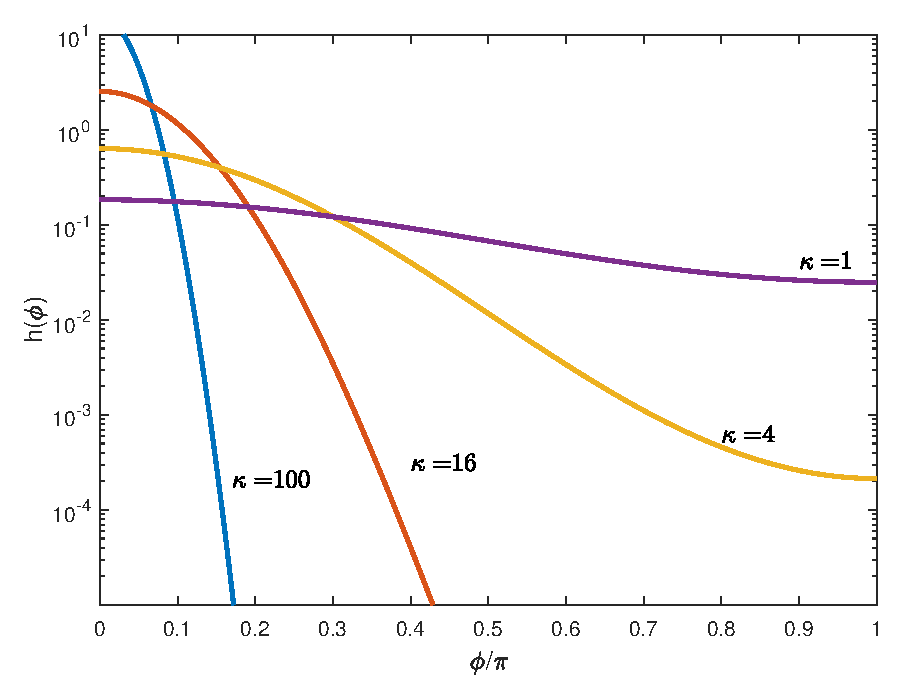
\includegraphics[width=0.6\textwidth]{figure/chapter4/FishVon_2D}
\caption{一维球体~$\mathbb{S}^{1}$~窗函数 }
\label{fig:Fishon_2D}
\end{figure}

本文中,在对原始声场进行空域加窗时,关于窗函数的选取原则如下:

(1)窗函数的主瓣方向:选取该时频点上平面波的来波方向,即球谐域~MUSIC~算法的结果;

(2)集中因子~$\kappa$:需要根据频率进行选择。设定目标半径~$R_{T}$,对于某一频率~$f$~,根据~$N_{T} = k R_{T} = 2\pi f R_{T}$~计算目标阶次,选择合适的集中因子~$\kappa$~使窗函数的球谐系数在前~$N_{T}$~阶的累积能量达到总能量的~$90\%$(或~$99\%$~等其他接近于~1~的数值)。

接下来对窗函数的球谐系数获取方法进行简单介绍。在上述选取原则的指导下,已经可以得到空域窗函数的具体表达式,因此可以在空间上任意位置取采样。相比于麦克风阵列的球谐系数获取,窗函数球谐系数的获取不受空间采样点数的限制,因此可以直接采用式~\eqref{eq.HRTF_Pinv}~的方式进行求解。


\section{整体算法框架}

基于球谐分解的双耳渲染算法直接在球谐域进行处理,如前所述,实际系统中录制声场的阶次受硬件设备的限制,因此和~HRTF~数据之间存在不匹配问题,HRTF~的直接低阶截断会对双耳信号带来损伤。本文所提出的算法分别从声场和~HRTF~两方面出发,共同解决二者之间的不匹配问题。接下来将对本文的内容进行总结,包括第~\ref{sec.SHdecomposition}~节、第~\ref{chapter.HRTF}~章和第~\ref{chapter.AddWindow}~章。


首先,第~\ref{sec.SHdecomposition}~节中对基于球谐分解的双耳渲染算法框架进行了详细介绍,给出了如何利用声场和~HRTF~的球谐系数获取双耳信号的方法。
第~\ref{chapter.HRTF}~章首先介绍了声场和~HRTF~球谐系数的获取方法,接下来引入了相位对准的~HRTF~预处理方法,并通过实验验证了该方法可以有效降低~HRTF~的球谐分解阶次。
第~\ref{chapter.AddWindow}~章创新性提出通过空域加窗的方法来提升录制声场的阶次。首先对信号模型及球谐域~MUSIC~定位算法进行了介绍,接下来对空域加窗可以实现声场阶次提升的原理进行推导,并对所采用的窗函数加以介绍。

以上三部分是本算法的理论基础,接下来给出引入声场扩阶和~HRTF~预处理的基于球谐分解的双耳渲染算法流程,如图~\ref{fig:algorithm}~所示。其中,STFT~和~ISTFT~分别为短时傅里叶变换及其逆变换,SFT~为球傅里叶变换。

\begin{figure}[H]
\centering
\includegraphics[width=0.88\textwidth]{figure/chapter4/algorithm}
\caption{引入声场扩阶和~HRTF~预处理的基于球谐分解的双耳渲染算法流程图}
\label{fig:algorithm}
\end{figure}

\section{本章小结}
本章对同时引入声场扩阶和~HRTF~预处理的基于球谐分解的双耳渲染算法进行了详细介绍。首先对信号模型进行描述,并给出了球谐域~MUSIC~定位算法以获取单时频点上的平面波来波方向。其次从有界线性算子出发,在球谐域上对加窗后信号的球谐系数表达式进行详细推导,并通过分析发现空域加窗可以实现声场阶次的提升。接下来对采用的窗函数及其选取原则和球谐系数求解方法加以介绍。最后将前三节的声场扩阶和第三章的~HRTF~预处理相结合,给出了总体算法框架。



\chapter{ 实验结果及分析 }

随着越来越多的技术进入消费者市场,有必要评估沉浸式音频体验的质量,以量化和优化技术,提高听众体验的真实性。质量评价的目的是测量听者对虚拟听觉环境的感知。在评价双耳沉浸式环境的质量时,我们需要考虑各种物理特征,包括声源定位精度、感知声源宽度(Apparent Source Width,ASW)、音质质量和损伤以及室内声学和环境相关属性~\tcite{2002Spatial}。

本章首先对评价指标及其计算方法进行详细介绍,主要包括声源定位精度和感知声源宽度两方面。然后从实验的角度出发,对本文所提出的双耳渲染算法的性能进行评估。

\section{ 评价指标 }\label{sec.evaulation}

声源定位是听众通过确定方位角、仰角和距离来定位声源的能力。在声源定位精度方面,主要采用的指标为双耳时间差~ITD~和双耳声级差~ILD~。瑞利在~1907~年将双耳时间差~ITD~和双耳声级差~ILD~引入作为声源定位因素,称为瑞利双因素理论。
该理论指出人耳听觉系统可以利用低频的~ITD~信息和高频的~ILD~信息决定声源方向。

感知声源宽度是对声源或声场在感知听觉宽度这一属性上的度量。这一主观属性与一种客观测量相关,最明显的是双耳听觉互相关系数。因此在空间感的感知方面,主要采用的指标为双耳听觉互相关系数~IACC。大量的主客观实验数据显示,双耳听觉互相关系数与声重放的空间主观感知有很强的相关性,可以用来衡量感知声源宽度。双耳听觉互相关系数定义为双耳归一化互相关函数的最大值,与空间感主观评测呈现负相关关系,即~IACC~值越小,双耳信号相关性越差,对应的声场越趋向于扩散场,因此感知声源更宽。

接下来将对三个指标的计算方法进行详细介绍。

\subsection{ 双耳时间差 }

双耳时间差(Interaural~Time~Difference,~ITD)是对声源方向定位的一个重要因素,其主要作用于低频段范围(小于~1.5~kHz),其表示的是声波从声源到双耳传输的时间差。
当声源位于中垂面(原点指向正前方和正上方的两个矢量构成的平面)时,声波从声源到达双耳的距离相等,传输所需的时间也相等,此时~ITD~为~0~。当声源偏离中垂面时,声波到达左、右耳的距离不同,对应的时间不同,此时双耳时间差不再为~0。

以水平面为例,如果不考虑头部对时间差的影响,可以将双耳近似为空间中相距~$2a$~的两点,如图~\ref{fig:ITD_compute}~中左图所示。则对于来波方向为~$\phi$~的远场平面波,其到达双耳的距离差为~$2a\sin\phi$,双耳时间差为:
\begin{equation}\label{ITD_1}
\text{ITD}(\phi)=\frac{2a}{c}\sin\phi
\end{equation}
式中:$c$~为声速。$\text{ITD}>0$~表示右耳比左耳先到达;$\text{ITD}<0$~正好相反。

如果考虑头部对时间差的影响,可以用刚球模型来近似人头,球面上相对的两点分别表示左右耳,如图~\ref{fig:ITD_compute}~中右图所示。该模型考虑了声波在头部弯曲表面~$a\phi$~的传输时间,此时式~\eqref{ITD_1}~可写为:
\begin{equation}\label{ITD_2}
\text{ITD}(\phi)=\frac{a}{c}(\sin\phi+\phi),~~~~~ 0\leq \phi \leq \frac{\pi}{2}
\end{equation}
上式给出了部分入射角的~ITD~计算公式,其他入射角的公式可以通过对称性得到。式~\eqref{ITD_2}~被称为~Woodworth~公式。

\begin{figure}[H]
\centering
\includegraphics[width=0.9\textwidth]{figure/chapter5/ITD_compute_theory}
\caption{ITD计算示意图\tcite{book_xiebosun}}
\label{fig:ITD_compute}
\end{figure}

当信号从正前方附近入射时,$\sin\phi\approx\phi$~,式~\eqref{ITD_1}~和~\eqref{ITD_2}~结果近似相等。
但对于其他角度,式~\eqref{ITD_1}~和~\eqref{ITD_2}~结果有一定差别。并且式~\eqref{ITD_1}~和~\eqref{ITD_2}~只适用于求解已知声源方位角时的理论~ITD~,对于一个未知声源方位的双耳信号,需要使用下述的三种方法进行求解。

(1)时域互相关法:

假设声源在左右耳产生的声压为~$b_{\text{L}}(t)$~和~$b_{\text{R}}(t)$,两路信号的互相关函数为:
%\begin{equation}\label{eq.IACC_ITD_1}
%\psi_{\text{LR}}(\tau) = \frac{\int_{t_{1}}^{t_{2}} b_{\text{L}}(t)b_{\text{R}}(t+\tau)dt}{\sqrt{\int_{t_{1}}^{t_{2}} b_{\text{L}}^{2}(t)dt\int_{t_{1}}^{t_{2}} b_{\text{R}}^{2}(t)dt}}
%\end{equation}

\begin{equation}\label{eq.IACC_ITD_1}
\psi_{\text{LR}}(\tau) = \frac{\int_{-\infty}^{\infty} b_{\text{L}}(t+\tau)b_{\text{R}}(t)dt}{\sqrt{\int_{-\infty}^{\infty} b_{\text{L}}^{2}(t)dt ~ \int_{-\infty}^{\infty} b_{\text{R}}^{2}(t)dt}}
\end{equation}

如果两路信号的时域表示为~$b_{{\text{L}}}(t)=g _{{\text{L}}} s(t+t_{{\text{L}}})+n_{{\text{L}}}(t)$,$b_{{\text{R}}}(t)=g _{{\text{R}}} s(t+t_{{\text{R}}})+n_{\text{R}}(t)$,$g _{{\text{L}}}$~与~$g _{{\text{R}}}$~分别反映声源信号~$s(t)$~到达左右耳处的幅度衰减函数,$t_{\text{L}}$~和~$t_{\text{R}}$~分别表示声源到达左右耳处所需的时间。由于~$n_{{\text{L}}}(t)$~和~$n_{{\text{R}}}(t)$~为加性随机噪声,与声源信号不相关,且互相独立,因此:
\begin{align}
     \psi_{{\text{L}}{\text{R}} }(\tau)&=g_{\text{L}} g_{\text{R}}r_{ss}(\tau-t_{\text{L}}+t_{\text{R}})+g _{\text{L}}r_{sn_{\text{R}}}(\tau-t_{\text{L}})+g_{\text{R}}r_{sn_{\text{L}}}(\tau+t_{\text{R}})+r_{ n_{\text{L}}n_{\text{R}}}  \nonumber \\
     &=g_{\text{L}} g_{\text{R}} r_{ss}(\tau-t_{\text{L}}+t_{\text{R}}),
\end{align}
其中,$r_{ss}$~和~$r_{ n_{\text{L}}n_{\text{R}}}$~分别表示信号的自相关函数和噪声的互相关函数,$r_{sn_{\text{L}}}$~和~$r_{sn_{\text{R}}}$~表示信号与噪声的互相关函数。

由互相关函数的性质可知,当~$\tau=t_{{\text{L}}}-t_{{\text{R}}}$~时,互相关函数~$\psi_{{\text{L}}{\text{R}}}(\tau)$~取最大值。所以双耳信号~$b_{\text{L}}(t)$~和~$b_{\text{R}}(t)$~之间的时延估计值为:
\begin{equation}
     \hat{\tau}_{\text{L}\text{R}}=\arg \max \limits_{\tau}~\psi_{\text{L}\text{R}}(\tau),
\end{equation}
式中,$\tau\in[-\tau _\text{max},\tau _\text{max}]$,$\tau _\text{max}$~在双耳信号计算中一般取~$1~\mathrm{ms}$。在麦克风阵列中,$\tau_{max}$~与阵元间距、声速和采样频率有关。

(2)频域相干法~\tcite{fangyi}:

对左右耳信号~$b_{\text{L}}(t)$~和~$b_{\text{R}}(t)$~进行短时傅里叶变换~(STFT)~转换到频域,表示为~$B_{\text{L}}(\mathscr{T},f)$~和~
$B_{\text{R}}(\mathscr{T},f)$,其中~$\mathscr{T}$~为时间帧,$f$~为频率。

两路信号之间的频域相干函数定义为:
\begin{equation}
\Gamma_{B_{\text{L}} B_{\text{R}}}(\mathscr{T},f)=\frac{P_{B_{\text{L}}B_{\text{R}}}(\mathscr{T}, f)}{\sqrt{P_{B_{\text{L}}B_{\text{L}}}(\mathscr{T}, f) P_{B_{\text{R}}B_{\text{R}}}(\mathscr{T},f)}},
\end{equation}
其中,$P_{B_{\text{L}}B_{\text{L}}}(\mathscr{T}, f)$~和~$P_{B_{\text{R}}B_{\text{R}}}(\mathscr{T},f)$~分别为 $B_{\text{L}}(\mathscr{T},f)$~和~
$B_{\text{R}}(\mathscr{T},f)$~的自功率谱,$P_{B_{\text{L}}B_{\text{R}}}(\mathscr{T},f)$~为 $B_{\text{L}}(\mathscr{T},f)$~
和 $B_{\text{R}}(\mathscr{T},f)$~的互功率谱,计算公式为:
\begin{align}
P_{B_{\text{i}}B_{\text{i}}}(\mathscr{T},f)
& =\alpha P_{B_{\text{i}}B_{\text{i}}}(\mathscr{T}-1,f)+
(1-\alpha)\left|B_{\text{i}}(\mathscr{T}, f)\right|^{2}, \quad i=\text{L},\text{R} \nonumber \\
P_{B_{\text{L}}B_{\text{R}}}(\mathscr{T},f) & =\alpha P_{B_{\text{L}}B_{\text{R}}}(\mathscr{T}-1,f)+
(1-\alpha) B_{\text{L}}(\mathscr{T},f) B_{\text{R}}^{*}(\mathscr{T},f)
\end{align}
其中 $\alpha$ 为相邻帧之间的平滑因子。

理想情况下单个声源在两个麦克风处的相干函数为:
\begin{equation}
\Gamma(f) = e^{j2\pi f\tau}
\end{equation}
当频率固定时,理想相干函数仅与时间差~$\tau$~有关。

此时,可以使用双耳信号的相干函数与多个~$\tau$~构成的理想相干函数库进行匹配,二者相关系数最高时所对应的~$\tau$~即为双耳信号的~ITD。也可以计算双耳信号相干函数的相位~$\psi$~,此时某个频点下的~ITD~为:
\begin{equation}
\text{ITD} = \frac{\psi}{2\pi f}
\end{equation}

\newpage
(3)改进的频域相干法:

在频域相干法中,使用关心频段内的所有频率进行~ITD~的计算,本方法对其改善,加入频率有效性判断。在每个频率计算一个频域相干函数,利用频率相干函数的幅度值大小判断该频率的有效性。当某个频率的相干函数幅度高于频段内幅度均值时,则认为该频率有效,最后只采用相关性大的频率进行~ITD~的求解。此种方法可以选取更为可靠的频率进行计算,降低了干扰频率带来的影响,从而进一步提高~ITD~计算结果的准确性和可靠性。

上文对三种计算~ITD~的方法进行了详细介绍,需要注意的是~ITD~是在低频段对声源定位的主要因素,所以在计算时需要对信号加以处理。对于时域计算方法,需要对双耳信号进行截止频率为~1.5~kHz~的低通滤波;对于频域计算方法,只需要对~1.5~kHz~以下的频率进行计算。

\subsection{ 双耳声级差 }

双耳声级差(Interaural~Level~Difference,~ILD)是声源方向定位的另一个重要因素,其主要作用于中高频,这是由于头部对声波有一定的反射和散射作用,高频时其作用更加明显。当声源偏离中垂面时,与声源同侧耳处的声压有所提升,异侧耳的声压有所衰减。因此,双耳声级差是声源方向和频率的函数。在单声源情况下,ILD~在低频时很小,且基本不随声源方向的改变而改变。随着频率的增加,ILD~逐渐增加,表现出与声源方向及频率的复杂关系~\tcite{book_xiebosun}。心理声学表明,大约在~1.5~kHz~以上,ILD~才开始作为一个有效的方向定位因素。

对于一个双耳信号,ILD~在某个频率~$f$~处的计算方式为:
\begin{equation}
\text{ILD}(f)=20\text{lg}\left|\frac{B_{\text{R}}(f)}{B_{\text{L}}(f)}\right|
\end{equation}
式中,~$B_{\text{R}}(f)$~和~$B_{\text{R}}(f)$~分别是左耳信号和右耳信号的频域声压。ILD~$> 0$~表示右耳比左耳先到达,ILD~$< 0$~相反。

有时也需要计算一定频率范围 $f_{\mathrm{L}} \leqslant f \leqslant f_{\mathrm{H}}$~内的平均双耳声级差,通过分别计算左右耳信号在某个频段内的总能量来获取~ILD:
\begin{equation}\label{eq.ILD_band}
\operatorname{ILD} =10 \text{lg} \left( \frac{\int_{f_{\mathrm{L}}}^{f_{\mathrm{H}}}\left|B_{\mathrm{L}}\left( f \right)\right|^{2} d f}{\int_{f_{\mathrm{L}}}^{f_{\mathrm{H}}}\left|B_{\mathrm{R}}\left(f \right)\right|^{2} d f} \right)
\end{equation}
在上式中选择不同的频率积分范围,即可得到该频带内的平均 ~ILD,例如,1/3~倍频程带。

在实际计算过程中,需要对式~\eqref{eq.ILD_band}~离散化求解:
\begin{equation}
\operatorname{ILD} =10 \text{lg} \left(\frac{ \sum_{f_{\mathrm{L}}}^{f_{\mathrm{H}}}\left|B_{\mathrm{L}}\left( f \right)\right|^{2} } { \sum_{f_{\mathrm{L}}}^{f_{\mathrm{H}}}\left|B_{\mathrm{R}}\left(f \right)\right|^{2} }\right)
\end{equation}

与~ITD~的计算相似,ILD~是声源在中高频段定位的主要因素,因此在计算过程中应该选取~1.5~kHz~以上的频率。由于语音的常用采样率为~16~kHz~,因此本文最终选取~$1.5\sim 8$~kHz~频段进行平均~ILD~的计算。

\subsection{ 双耳相关性 }
在室内声学中,空间感(Spaciousness)是总体空间印象的一个重要部分,是衡量厅堂音质的重要主观评价指标。
% 室内不同的时空设置可以影响距离感知和声像拓宽,以及沉浸或被声音包围的感觉,因而也有人将空间感称为感知声源宽度。
大量的研究表明,厅堂的早期反射对于空间感至关重要,特别是~1.5~kHz~以下的低频成分。Amdo~的研究表明厅堂的空间感与分立反射声的空间方向分布有关,并提出以双耳听觉互相关系数~\tcite{book_xiebosun}(Interaural Cross-Correlation,IACC)作为衡量空间感的一个客观指标。

IACC~是双耳信号空间感评测的重要指标,同时可以用于预测感知声源宽度。其测量两个耳朵信号的相似度, 通过计算双耳信号的归一化互相关函数的最大值而来,互相关分析用于表明在给定的一段时间内两个时域波形的相似程度。 归一化互相关函数定义如式~\eqref{eq.IACC_ITD_1}~所示,通常最大化互相关是在~$-1\mathrm{~ms} \leq \tau \leq 1\mathrm{~ms} $~范围内计算~$\psi_{\text{LR}}(\tau)$~的最大值:
\begin{equation}
\mathrm{IACC} = \underset{-1 \mathrm{~ms}~<~\tau~<~1 \mathrm{~ms}}{\operatorname{max}} ~~\psi_{\text{LR}}(\tau)
\end{equation}

由定义可知,所有的~$0 \leq \text{IACC} \leq 1$。IACC~为~1~表示两个信号完全相关,当信号具有较低的相似度或存在随机相关时,IACC~趋近于~0。

有时还会引入半波整流和低通滤波以模拟在高频时听觉系统中发生的包络提取,这种改进的早期~IACC~称为~$\mathrm{IACC}_{E}$,更适合预测~ASW。与~ITD~类似,本文在计算~IACC~前对信号进行截止频率为~1.5~kHz~的低通滤波。

最小可觉差(Just Noticeable Difference,JND)也被称为差别阈值线,体现人们对改变或者误差的容忍度,是测量两种事物差异的数量单位。如果误差~$\Delta$~和~JND~之比小于~1,即~$\Delta$~小于~JND,可以近似认为二者在感知上无差别。

对于~IACC~来说,其最小可觉差~\tcite{2018comparison}\tcite{JND}可以通过下式计算:
\begin{equation}\label{eq.JND_IACC}
\mathrm{JND}(x)=\max \left( 0.557-0.379 x-0.178 x^{2}~, ~0.007 \right)
\end{equation}
其中,$x$~表示参考双耳信号的~IACC。

为了避免在相除过程中~JND~作为分母取值为~0,对最小值加以约束,即式~\eqref{eq.JND_IACC}~中的限制~JND$(0.99)=0.007$。


\section{实验结果及分析}

在本节中,将使用第~\ref{sec.evaulation}~节所介绍的评价指标对本文所提出的方法进行评估。接下来对参与评估的算法和信号进行简单介绍。

首先,选取了一个参考信号,其声场和~HRTF~的球谐分解均为~34~阶,并且麦克风阵列半径为~0.1~米(接近人头尺寸),参见式~\eqref{eq.BL}~和式~\eqref{eq.BR}~获取双耳信号,记作~Original。参与比较的算法包括以下三个:

\begin{inparaenum}[(1)]

\item 直接基于低阶球谐分解的双耳渲染算法。声场的球谐分解为~$N_{s}$~阶,HRTF~直接进行低阶截断,且球谐分解的阶次与声场保持一致,记作~LS;

\item 引入~HRTF~预处理的双耳渲染算法。声场的球谐分解为~$N_{s}$~阶,对~HRTF~进行相位对准预处理,使其能量更加集中在低频,HRTF~的球谐分解阶次仍为~$N_{s}$~阶,记作~HRTF Pre~;

\item 同时引入声场扩阶和~HRTF~预处理的双耳渲染算法。将声场的球谐分解阶次从~$N_{s}$~提升为~$N_{T}$~阶,并对~HRTF~进行相位对准预处理,且球谐分解阶次为~$N_{T}$~阶,记作~EO+HRTF Pre,其中~EO~表示扩阶(Enalrge Order)。

\end{inparaenum}

\subsection{消声室环境下各算法性能对比}

仿真环境为消声室环境,麦克风阵列采用~Eigenmike~球阵,其包含~32~个麦克风,半径为~0.042~米,对应的球谐函数分解阶次~$N_{s}=4$~阶。麦克风阵列和声源位于同一水平面,即俯仰角为~$\theta=90^{\circ}$~,且相距~2~米。声源以~Eigenmike~为圆心均匀运动,即声源相对麦克风阵列的方位角~$\phi$~均匀变化。方位角~$\phi$~的取值范围从~$0^{\circ}$(即正前方)沿顺时针方向到~$90^{\circ}$(即正右方),角度间隔为~$10^{\circ}$,其它方位的结论可以较为容易地通过对称来获取。
声源信号包括两类,白噪声信号和语音信号。

消声室情况下,主要采用双耳时间差~ITD~和双耳声级差~ILD~这两个评价指标,并且通过计算和对比三种待评估算法~(~LS、HRTF Pre~和~EO+HRTF Pre)~对应的双耳信号与参考双耳信号~Original~在~ITD~和~ILD~上的误差~$\Delta_{\text{ITD}}$~和~$\Delta_{\text{ILD}}$~来进行评估,如式~\eqref{eq.delta_ITDILD}~所示。误差越小,则认为该算法越优。
\begin{align}\label{eq.delta_ITDILD}
\Delta_{\text{ITD}}  &= \left|~ \text{ITD}_{\text{case}} - \text{ITD}_{\text{Original}} ~\right| \nonumber\\
\Delta_{\text{ILD}}  &= \left|~ \text{ILD}_{\text{case}} - \text{ILD}_{\text{Original}} ~\right|
\end{align}
其中,case~表示~LS、HRTF Pre~和~EO+HRTF Pre。


不同声源类型(白噪声、语音)、不同方位角对双耳信号的影响如图~\ref{fig.xiaoshengshi_eigenmike_phiChange_whitenoise}~所示,图~(a)~和图~(b)~为声源为白噪声信号,位于不同方位角时三种算法对应的双耳信号的~$\Delta_{\text{ITD}}$~和~$\Delta_{\text{ILD}}$~结果,图~(c)~和图~(d)~为声源为语音信号,位于不同方位角时三种算法对应的双耳信号的~$\Delta_{\text{ITD}}$~和~$\Delta_{\text{ILD}}$~结果。

\begin{figure}[H]
\centering
\subfigure[]{
\includegraphics[width=0.48\textwidth]{error_ITD_xiaoshengshi_eigenmike_phiChange_whitenoise}}
\hfill
\subfigure[]{
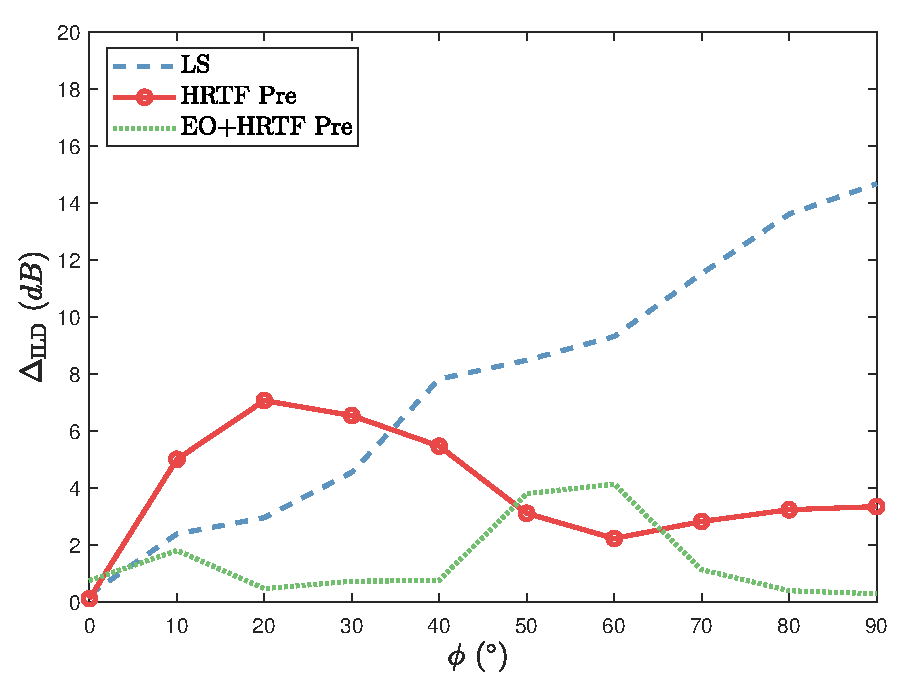
\includegraphics[width=0.48\textwidth]{error_ILD_xiaoshengshi_eigenmike_phiChange_whitenoise}}
\vfill
\subfigure[]{
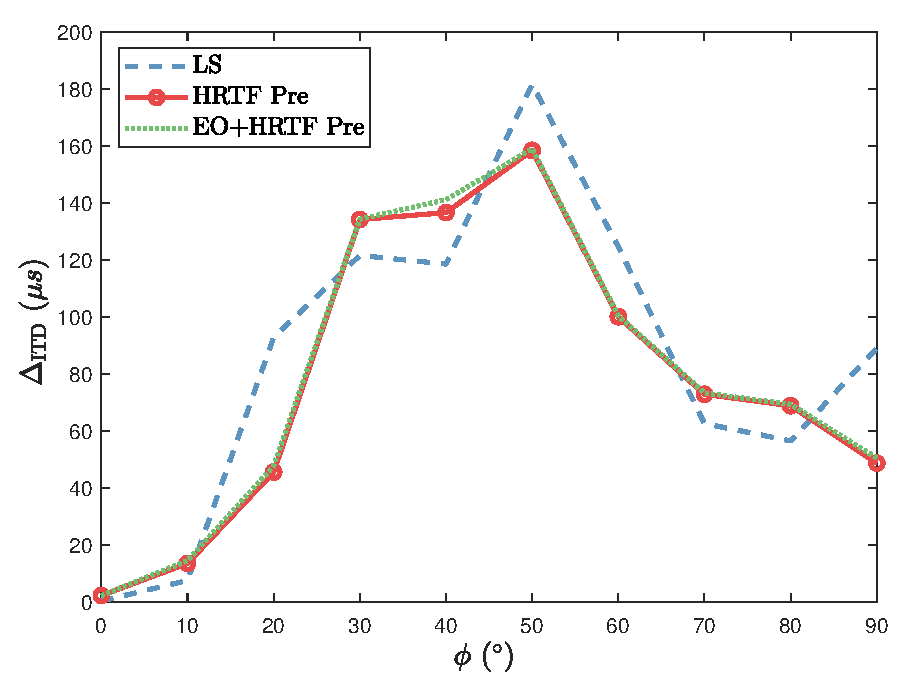
\includegraphics[width=0.48\textwidth]{error_ITD_xiaoshengshi_eigenmike_phiChange_audio}}
\hfill
\subfigure[]{
\includegraphics[width=0.48\textwidth]{error_ILD_xiaoshengshi_eigenmike_phiChange_audio}}
\caption{消声室环境下两种声源信号在不同方位角处的实验结果:白噪声:~(a)~ITD;(b)~ILD;语音:~(c)~ITD;(d)~ILD}
\label{fig.xiaoshengshi_eigenmike_phiChange_whitenoise}
\end{figure}


从图~\ref{fig.xiaoshengshi_eigenmike_phiChange_whitenoise}~可以看出:
\begin{inparaenum}[(1)]

\item 无论是白噪声信号还是语音信号,LS、HRTF Pre~和~EO + HRTF Pre~算法的~$\Delta_{\text{ITD}}$~结果基本一致,这是因为~HRTF Pre~算法进行相位对准的起始频率为~1.5~kHz,EO + HRTF Pre~算法在引入声场扩阶的过程中,当~$N_{T}>N_{s}$~时才开始进行处理,根据~$N_{T} =k R_{T}=2\pi f R_{T}/c$,$R_{T}=0.1$~米和原有声场阶次~$N_{s}=4$~阶可知,进行声场扩阶的起始频率为~2.7~kHz。而评价指标~ITD~的关注频率范围为~1.5~kHz~以下,此频段内~HRTF Pre~和~EO + HRTF Pre~算法并未对双耳信号进行任何处理,因此三种算法的~$\Delta_{\text{ITD}}$~结果没有区别。

\item 无论是白噪声信号还是语音信号,EO + HRTF Pre~算法的~$\Delta_{\text{ILD}}$~结果最小,并且在任意方位角下均可达到较小的误差。LS~算法与~Original~的差距最大,且随着方位角的变化,误差一直增大。

\item 相较于~LS~算法,HRTF Pre~算法在大多数方位角下的~$\Delta_{\text{ILD}}$~有所降低,更加接近~Originial~算法,但是在部分角度($10^{\circ}$、$20^{\circ}$)HRTF Pre~算法的误差大于~LS~算法,进一步分析发现~HRTF Pre~算法在这些角度出现~ILD~的正负错误,可能会带来少量的声源定位错误,而改进方法~EO + HRTF Pre~并未出现此问题。

\item 相比于白噪声信号,语音信号的~ITD~和~ILD~结果有少许变化,这是因为语音信号的能量主要集中在低频,并且在各频点上的能量分布不均,而白噪声在整个频谱上均匀分布,避免了计算波动。但是两种声源类型对应的综合结论一致。

\end{inparaenum}

上图展示了~1.5~kHz~到~8~kHz~频段内平均~ILD~的结果,接下来以方位角~$\phi=40^{\circ}$~为例,对三种算法所获取的双耳信号与参考信号在~8~kHz~以下频段内单个频点处的~$\Delta_{\text{ILD}}$~结果进行展示,如图~\ref{fig:xiaoshengshi_eigenmike_40du}~所示。

\begin{figure}[!h]
\centering
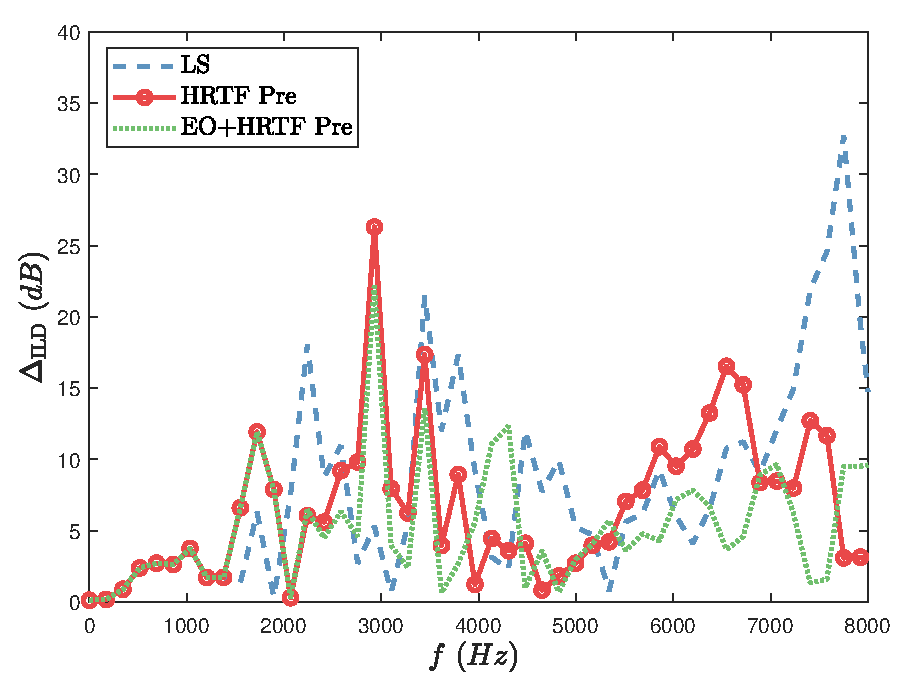
\includegraphics[width=0.6\textwidth]{error_xiaoshengshi_eigenmike_40du}
\caption{消声室情况下方位角~$\phi=40^{\circ}$~时单个频点处的~$\Delta_{\text{ILD}}$~结果}
\label{fig:xiaoshengshi_eigenmike_40du}
\end{figure}

从图~\ref{fig:xiaoshengshi_eigenmike_40du}~可以看出:

\begin{inparaenum}[(1)]

\item 综合整个频段来看, EO + HRTF Pre~算法的~$\Delta_{\text{ILD}}$~结果最小,尤其是在~5~kHz~以上的高频,现有的研究表明,ILD~是高频定位因素,1.5~kHz以上~ILD~才开始对定位起作用,频率大于~4~kHz~时,ILD~才是方向定位的主要因素。HRTF Pre~算法次之,LS~算法的~ $\Delta_{\text{ILD}}$~最大,与图~\ref{fig.xiaoshengshi_eigenmike_phiChange_whitenoise}~中~1.5~kHz~到~8~kHz~频段内平均~$\Delta_{\text{ILD}}$~的结论一致。

\item 相比于~LS~算法,HRTF Pre~和~EO + HRTF Pre~算法的~ILD~开始在~1.5~kHz~有所调整。相比于~HRTF Pre~算法,EO + HRTF Pre~算法的~ILD~开始在~2.7~kHz~有所调整,与图~\ref{fig.xiaoshengshi_eigenmike_phiChange_whitenoise}~的讨论中频率相关的结论一致。
\end{inparaenum}





\subsection{空心球与刚性球的性能对比}\label{subsec.open_rigid}

仿真环境为消声室环境,麦克风阵列采用含有~32~个麦克风的空心球阵,对应的球谐函数分解阶次~$N_{s}=4$~阶。空心球阵的半径从~0.01~米到~0.1~米均匀取值,间隔为~0.01~米。麦克风阵列和声源位于同一水平面,俯仰角为~$\theta=90^{\circ}$,且相距~2~米,声源位于麦克风阵列的正右方,即方位角~$\phi=90^{\circ}$。
声源信号包括两类,白噪声信号和语音信号。

不同声源类型(白噪声、语音)、不同麦克风阵列半径~$R$~对双耳信号的影响如图~\ref{fig.xiaoshengshi_eigenmike_r_eigChange_whitenoise}~所示,其中图~(a)~和图~(b)~是声源为白噪声信号,采用不同麦克风阵列半径时三种算法对应的双耳信号与参考双耳信号之间的~$\Delta_{\text{ITD}}$~和~$\Delta_{\text{ILD}}$~结果,图~(c)~和图~(d)~是声源为语音信号,采用不同麦克风阵列半径时三种算法的~$\Delta_{\text{ITD}}$~和~$\Delta_{\text{ILD}}$~结果。

\begin{figure}[!h]
\centering
\subfigure[]{
\includegraphics[width=0.48\textwidth]{error_ITD_xiaoshengshi_eigenmike_r_eigChange_whitenoise}}
\hfill
\subfigure[]{
\includegraphics[width=0.48\textwidth]{error_ILD_xiaoshengshi_eigenmike_r_eigChange_whitenoise}}
\vfill
\subfigure[]{
\includegraphics[width=0.48\textwidth]{error_ITD_xiaoshengshi_eigenmike_r_eigChange_audio}}
\subfigure[]{
\includegraphics[width=0.48\textwidth]{error_ILD_xiaoshengshi_eigenmike_r_eigChange_audio}}
\caption{空心球情况下两种声源信号在不同麦克风阵列半径时的实验结果:白噪声:~(a)~ITD;(b)~ILD;语音:~(c)~ITD;(d)~ILD}
\label{fig.xiaoshengshi_eigenmike_r_eigChange_whitenoise}
\end{figure}

从图~\ref{fig.xiaoshengshi_eigenmike_r_eigChange_whitenoise} ~可以看出:
\begin{inparaenum}[(1)]

\item 无论是白噪声信号还是语音信号,LS、HRTF Pre~和~ EO + HRTF Pre~算法的~$\Delta_{\text{ITD}}$~结果完全一致,与图~\ref{fig.xiaoshengshi_eigenmike_phiChange_whitenoise}~的讨论一致。并且当麦克风阵列半径接近人头尺寸时,$\Delta_{\text{ITD}}$~达到较小的值。

\item 无论是白噪声信号还是语音信号,HRTF Pre~和~ EO + HRTF Pre~算法的~$\Delta_{\text{ILD}}$~结果远小于~LS~算法,且~ EO + HRTF Pre~算法更适合半径较小的空心球阵(小于等于~0.05~m),HRTF Pre~算法更适合尺寸较大的麦克风阵列。

\item 当麦克风阵列半径~$R$~大于等于~0.05~m~时,声场扩阶算法开始不起作用,甚至对~ILD~有一定的损伤,$\Delta_{\text{ILD}}$~大于~HRTF Pre~算法。这是因为空心球阵情况下会存在球贝塞尔函数零点问题,零点的引入会对声场扩阶算法中的球谐域~MUSIC~定位算法有影响,导致错误的声场扩阶。

\item 半径~$R=0.1$~米时,HRTF Pre~和~EO + HRTF Pre~算法的~$\Delta_{\text{ITD}}$~和~$\Delta_{\text{ILD}}$~结果完全一致,这是因为~EO + HRTF Pre~算法的目标球体半径~$R_{T}=0.1$,此时两种算法等效。

\end{inparaenum}

对球贝塞尔函数的零点进行进一步分析,图~\ref{fig.xiaoshengshi_r_eig_bessel_zero}~给出了~EO + HRTF Pre~算法在不同麦克风阵列半径下三种算法所获取的双耳信号与参考信号在~8~kHz~以下频段内单个频点处的~ILD~结果,以及~4~阶球贝塞尔函数~$j_{4}(kR)$~在不同半径~$R$~下随频率~$f$~的变化情况。

\begin{figure}[H]
\centering
\subfigure[]{
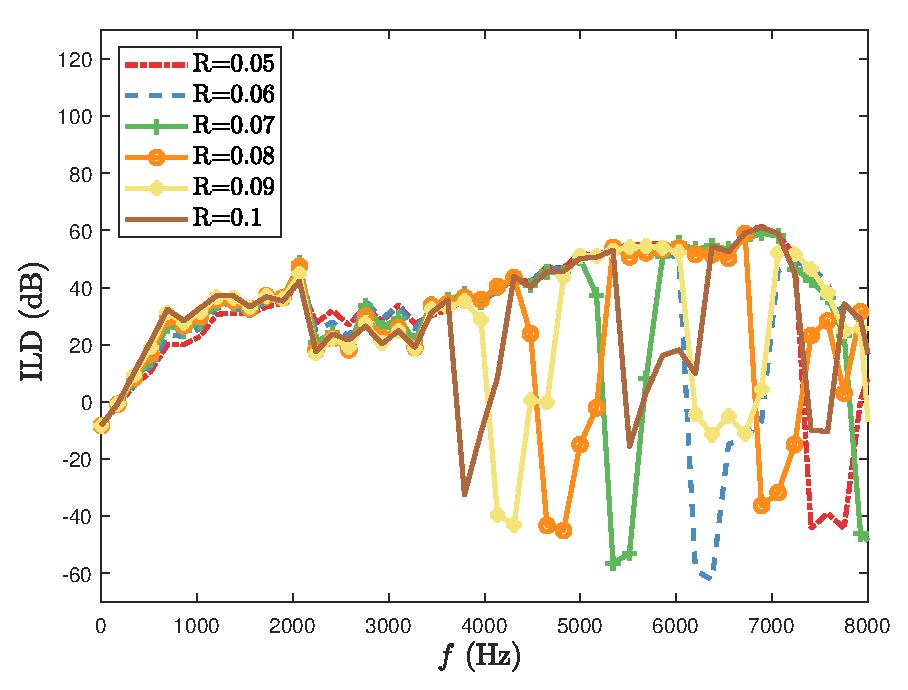
\includegraphics[width=0.48\textwidth]{xiaoshengshi_r_eig_bessel_zero}}
\hfill
\subfigure[]{
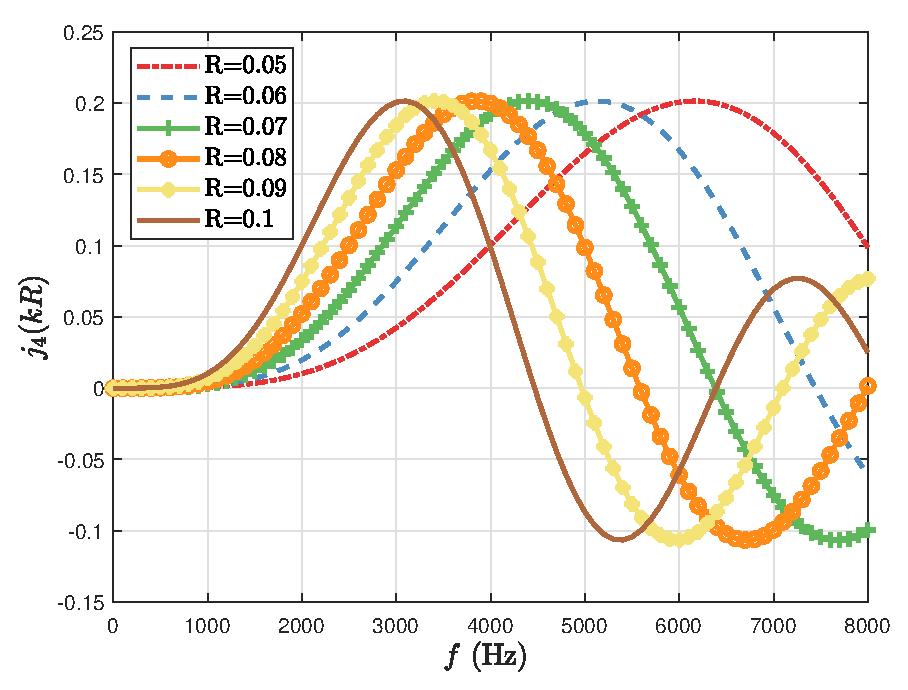
\includegraphics[width=0.48\textwidth]{bessel_4order}}
\caption{消声室情况下不同麦克风阵列半径在各个频点的~ILD~}
\label{fig.xiaoshengshi_r_eig_bessel_zero}
\end{figure}

从图~\ref{fig.xiaoshengshi_r_eig_bessel_zero}~可以看出:

\begin{inparaenum}[(1)]

\item 本实验中声源的方位角~$\phi=90^{\circ}$,ILD~应该为正值,而图~(a)~中部分频率的~ILD~出现负值,且其绝对值较大,严重影响了平均~ILD~结果,因此导致了图~\ref{fig.xiaoshengshi_eigenmike_r_eigChange_whitenoise} (b)~和~(d)~中的~ILD~损伤现象。

\item 对比图~(a)~和图~(b)~可以看出,固定麦克风半径~$R$,ILD~出现错误的频率位于该半径下球贝塞尔函数的零点处或零点附近,这是因为零点的存在导致球谐域~MUSIC~定位算法的错误,从而导致~ILD~错误。

\item 图~(b)~中,对于~4~阶球贝塞尔函数来说,$R\geq0.05$~时,零点开始出现在~8~kHz~以下的频段,且半径~$R$~越大,开始出现零点的频率越小,8~kHz~以下的频段零点出现的次数越多。这也导致了半径越大, EO + HRTF Pre~算法的~ILD~结果与~Original~算法的差距越大。
\end{inparaenum}



在第~\ref{section_microphone_array_coe}~节中对空心球和刚性球进行了详细讨论,并且已经从原理上证明,由于散射声场的存在,刚性球可以避免球贝塞尔函数的零点问题,从而解决空心球带来的一些问题,更加适用于实际系统。

接下来采用刚性球阵进行仿真实验,其余实验设置均保持不变,并且只关注~ EO + HRTF Pre~算法出现~ILD~损伤的情况,即麦克风阵列半径从~0.05~米到~0.1~米均匀取值,间隔为~0.01~米。
图~\ref{fig.rigid_xiaoshengshi_r_eig_whitenoise}~给出了刚性球情况下,不同声源类型和不同麦克风阵列半径下三种算法对应的双耳信号与参考双耳信号之间的~$\Delta_{\text{ITD}}$~和~$\Delta_{\text{ILD}}$~结果,图~\ref{fig:xiaoshengshi_rigid_ILD_fre}~给出了~EO + HRTF Pre~算法在采用不同麦克风阵列半径的刚性球情况下,三种算法所获取的双耳信号与参考信号在~8~kHz~以下频段内单个频点处的~ILD~结果。

\begin{figure}[H]
\centering
\subfigure[]{
\includegraphics[width=0.48\textwidth]{error_ITD_rigid_xiaoshengshi_r_eig_whitenoise}}
\hfill
\subfigure[]{
\includegraphics[width=0.48\textwidth]{error_ILD_rigid_xiaoshengshi_r_eig_whitenoise}}
\vfill
\subfigure[]{
\includegraphics[width=0.48\textwidth]{error_ITD_rigid_xiaoshengshi_r_eig_audio}}
\hfill
\subfigure[]{
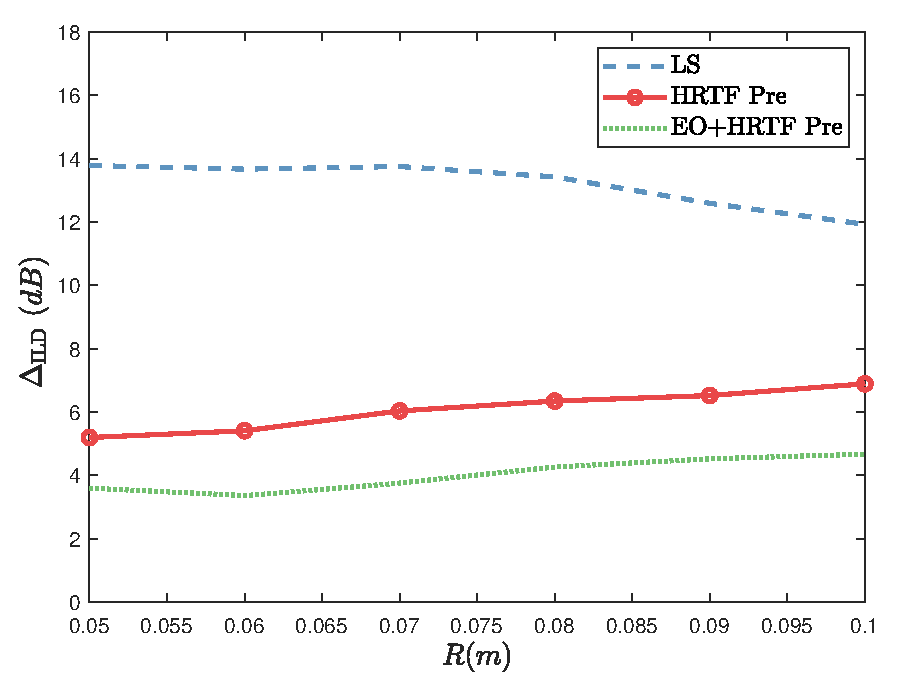
\includegraphics[width=0.48\textwidth]{error_ILD_rigid_xiaoshengshi_r_eig_audio}}
\caption{刚性球情况下两种声源信号在不同麦克风阵列半径时的实验结果:白噪声:~(a)~ITD;(b)~ILD;语音:~(c)~ITD;(d)~ILD}
\label{fig.rigid_xiaoshengshi_r_eig_whitenoise}
\end{figure}

\begin{figure}[H]
\centering
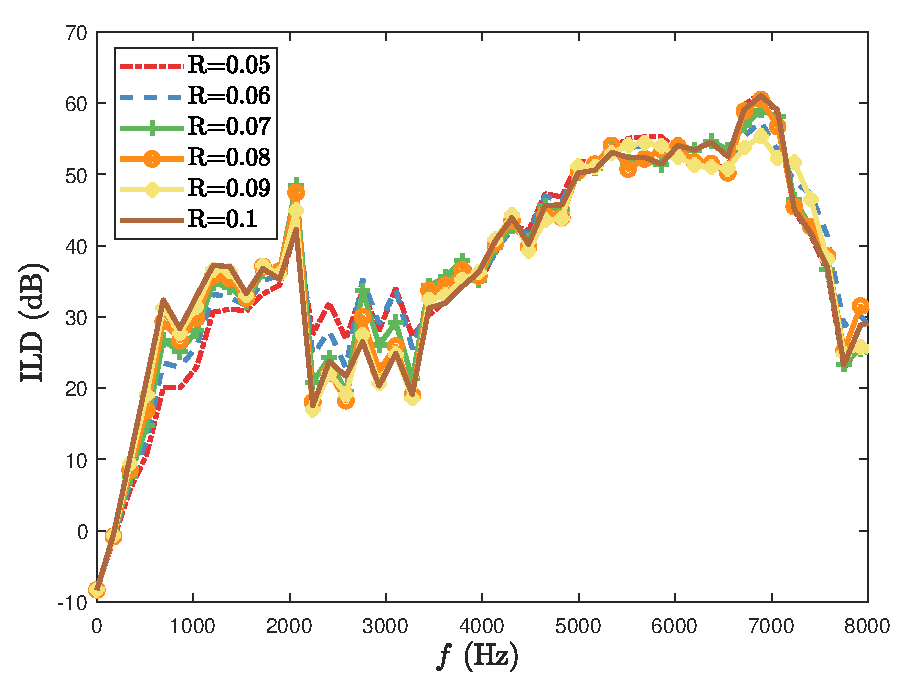
\includegraphics[width=0.6\textwidth]{xiaoshengshi_rigid_ILD_fre}
\caption{刚性球情况下采用不同麦克风阵列半径的单频点~ILD~结果}
\label{fig:xiaoshengshi_rigid_ILD_fre}
\end{figure}


从图~\ref{fig.rigid_xiaoshengshi_r_eig_whitenoise}~和~\ref{fig:xiaoshengshi_rigid_ILD_fre}~可以看出:

\begin{inparaenum}[(1)]

\item 无论是白噪声信号还是语音信号,刚性球情况下~EO + HRTF Pre~算法在各个半径的~$\Delta_{\text{ILD}}$~结果最小,HRTF Pre~算法次之,LS~算法的误差最大,且远大于~HRTF Pre~和~EO + HRTF Pre~算法。

\item 刚性球的使用避免了~EO + HRTF Pre~算法在空心球情况中较大的麦克风阵列半径下的~ILD~损伤现象,因此~EO + HRTF Pre~算法在刚性球情况下适用于研究范围内的任意半径。

\item 对比图~\ref{fig.xiaoshengshi_r_eig_bessel_zero}(a)~和~图~\ref{fig:xiaoshengshi_rigid_ILD_fre}~可以看出,刚性球可以避免球贝塞尔函数的零点给~EO + HRTF Pre~算法带来的~ILD~正负错误,体现了刚性球的优越性。

\end{inparaenum}

\subsection{混响环境下各算法性能对比}

本实验的仿真环境为混响环境,声源在混响室的传播可以用镜像模型方法(Image Source Method,ISM)产生~\tcite{1979Image}。
镜像模型方法通常以矩形结构房间为基本模型,可通过调节墙壁反射系数~$\beta$、房间尺寸大小、声源位置及麦克风接收位置等参数来获得房间冲激响应,目前已经广泛应用于各种仿真实验中。其基本思想是用虚拟镜像来等效地替代声源在墙壁发生的反射,进而确定反射声的传播路径,一旦确定房间设置(尺寸、反射系数)及声源与麦克风的位置,既可计算所有的镜像声源坐标和对应的能量衰减系数。

反射系数的取值范围是~$0$~到~$1$~之间,本文选取的反射系数为~$0$、$0.3$、$0.5$~和~$0.7$,分别对应无混响、低混响、中等混响和强混响的声学环境。混响的强弱也可以用混响时间~$T_{60}$~这一指标来描述,其表示的是在扩散声场中当声源停止后从初始的声压级衰减~60~dB~时所对应的时间,描述了室内混响声的衰减快慢。
常用的两个计算公式为艾润公式和赛宾公式~\tcite{book_xiebosun}:
\begin{align}
T_{60} & = 0.161 \frac{V}{-S ~\text{ln}(1-\alpha)} \nonumber\\
T_{60} & = 0.161 \frac{V}{S \alpha}
\end{align}
其中,$V$~为房间的体积,$S$~为总的吸声面积,$\alpha$~为平均吸声系数,$\alpha = 1-\beta^{2}$,$\beta$~为反射系数。

混响环境下~IACC~是一个重要评价指标,因此本实验中同时使用双耳时间差~ITD、双耳声级差~ILD~和双耳互相关系数~IACC~这三个评价指标对各种算法进行分析。和~$\Delta_{\text{ITD}}$、$\Delta_{\text{ILD}}$~类似,引入~$\Delta_{\text{IACC}}$:
\begin{align}\label{eq.delta_IACC}
\Delta_{\text{IACC}} &= \left|~\text{IACC}_{\text{case}} - \text{IACC}_{\text{Original}} ~\right|
\end{align}
其中,case~表示~LS、HRTF Pre~和~EO+HRTF Pre。

本实验选取尺寸为~$5~\mathrm m\times7~\mathrm m\times3~\mathrm m$~的房间,反射系数为~$0$、$0.3$、$0.5$~和~$0.7$。麦克风阵列采用~Eigenmike~球阵,其包含~32~个麦克风,对应的球谐函数分解阶次~$N_{s}=4$~阶,半径为~0.042~米。Eigenmike~位于房间中心,与声源处于~$z=1.5$~米的同一水平面上,且相距~2~米。声源位于麦克风阵列的正右方,即方位角~$\phi=90^{\circ}$。
声源信号包括两类,白噪声信号和语音信号。

不同声源类型(白噪声、语音)、不同反射系数对双耳信号的影响如表~\ref{tab:ITD}、\ref{tab:ILD}~和~\ref{tab:IACC}~所示,分别为三种算法对应的双耳信号与参考双耳信号之间的~$\Delta_{\text{ITD}}$、$\Delta_{\text{ILD}}$~和~$\Delta_{\text{IACC}}$~结果。表~\ref{tab:IACC}~中的~JND~为参考双耳信号~Original~的~IACC~对应的最小可觉差,参见式~\eqref{eq.JND_IACC}。

\begin{table}[H]
  \centering
  \caption{两种声源信号在不同反射系数下的~$\Delta_{\text{ITD}}~(\mu s)$~}
  {\zihao{5}
    \begin{tabular}{m{3cm}<{\centering}m{1cm}<{\centering}m{1cm}<{\centering}m{1cm}<{\centering}m{1cm}<{\centering}m{0.2cm}<{\centering}m{1cm}<{\centering}m{1cm}<{\centering}m{1cm}<{\centering}m{1cm}<{\centering}}
    \toprule[1.5pt]
     & \multicolumn{4}{c}{白噪声信号}~ & & \multicolumn{4}{c}{语音信号} \\
    \cmidrule{2-5}  \cmidrule{7-10}
    反射系数                    & 0 & 0.3  & 0.5 & 0.7 & & 0   & 0.3  & 0.5 & 0.7 \\ \hline
    LS            & 67 & 26  & 12  & 7   & & 163 & 12   & 6   & 4 \\ \hline
    HRTF Pre      & 66 & 27  & 14  & 8   & & 123 & 34   & 12  & 5 \\ \hline
    EO+HRTF Pre   & 66 & 27  & 14  & 7   & & 124 & 33   & 12  & 5 \\
    \toprule[1.5pt]
    \end{tabular}%
  }
  \label{tab:ITD}%
\end{table}%

从表~\ref{tab:ITD}~可以看出:无论是白噪声信号还是语音信号,三种算法在各个反射系数下的~$\Delta_{\text{ITD}}$~基本一致,语音信号情况下三种算法之间的误差相对较大,这是因为语音信号在各频点上的能量分布不均导致的计算波动。整体结论与之前的实验一致,HRTF Pre~和~EO+HRTF Pre~算法并未对~LS~算法的~ITD~加以改变。


\begin{table}[H]
  \centering
  \caption{两种声源信号在不同反射系数下的~$\Delta_{\text{ILD}}~(dB)$~}
  {\zihao{5}
    \begin{tabular}{m{3cm}<{\centering}m{1cm}<{\centering}m{1cm}<{\centering}m{1cm}<{\centering}m{1cm}<{\centering}m{0.2cm}<{\centering}m{1cm}<{\centering}m{1cm}<{\centering}m{1cm}<{\centering}m{1cm}<{\centering}}
    \toprule[1.5pt]
     & \multicolumn{4}{c}{白噪声信号}~ & & \multicolumn{4}{c}{语音信号} \\
    \cmidrule{2-5}  \cmidrule{7-10}
    反射系数                    & 0     & 0.3   & 0.5   & 0.7  & & 0     & 0.3   & 0.5   & 0.7 \\ \hline
    LS            & 14.8  & 9.3   & 6.4   & 3.6  & & 14.3  & 6.1   & 3.2   & 3.4  \\ \hline
    HRTF Pre      & 3.4   & 3.9   & 3.6   & 1.9  & & 5.8   & 2.1   & 1.9   & 0.7 \\ \hline
    EO+HRTF Pre   & 0.5   & 0.6   & 0.7   & 0.8  & & 4.6   & 0.4   & 2.1   & 1.9 \\
    \toprule[1.5pt]
    \end{tabular}%
  }
  \label{tab:ILD}%
\end{table}%


\begin{table}[H]
  \centering
  \caption{两种声源信号在不同反射系数下的~$\Delta_{\text{IACC}}$~}
  {\zihao{5}
    \begin{tabular}{m{3cm}<{\centering}m{1cm}<{\centering}m{1cm}<{\centering}m{1cm}<{\centering}m{1cm}<{\centering}m{0.2cm}<{\centering}m{1cm}<{\centering}m{1cm}<{\centering}m{1cm}<{\centering}m{1cm}<{\centering}}
    \toprule[1.5pt]
     & \multicolumn{4}{c}{白噪声信号}~ & & \multicolumn{4}{c}{语音信号} \\
    \cmidrule{2-5}  \cmidrule{7-10}
    反射系数                    & 0       & 0.3     & 0.5     & 0.7     & & 0       & 0.3     & 0.5     & 0.7 \\ \hline
    LS            & 0.2866  & 0.0775  & 0.0172  & 0.0017  & & 0.1066  & 0.0176  & 0.0040  & 0.0005  \\ \hline
    HRTF Pre      & 0.1897  & 0.0319  & 0.0076  & 0.0095  & & 0.0589  & 0.0018  & 0.0008  & 0.0011 \\ \hline
    EO+HRTF Pre   & 0.1866  & 0.0467  & 0.0028  & 0.0071  & & 0.0947  & 0.0153  & 0.0031  & 0.0001 \\ \hline
    JND           & 0.2847  & 0.0955  & 0.0260  & 0.0070  & & 0.1049  & 0.0220  & 0.0085  & 0.0070 \\
    \toprule[1.5pt]
    \end{tabular}%
  }
  \label{tab:IACC}%
\end{table}%

从表~\ref{tab:ILD}~可以看出:
\begin{inparaenum}[(1)]

\item 无论是白噪声信号还是语音信号,相较于~LS~算法,HRTF Pre~算法和~EO+HRTF Pre~算法的~$\Delta_{\text{ILD}}$~明显降低。

\item 对于白噪声信号,EO+HRTF Pre~算法的~$\Delta_{\text{ILD}}$~最小,小于~1~dB,HRTF Pre~次之,LS~算法的误差最大。 对于语音信号,不同混响情况下,HRTF Pre~和~EO+HRTF Pre~算法的差异不大。ILD~是一个高频定位因素,因此相对来说白噪声下的结果更为可靠,即~EO+HRTF Pre~算法最优。

\end{inparaenum}


从表~\ref{tab:IACC}~可以看出:
\begin{inparaenum}[(1)]

\item 无论是白噪声信号还是语音信号,在大多数混响环境下(反射系数为~0.7~除外),相较于~LS~算法,HRTF Pre~和~EO + HRTF Pre~算法的~$\Delta_{\text{IACC}}$~有所下降。

\item 反射系数为~0.7~时,对于白噪声信号,HRTF Pre~和~EO + HRTF Pre~算法的~$\Delta_{\text{IACC}}$~与~JND~基本一致,且大于~LS~算法。对于语音信号,三种算法的~$\Delta_{\text{IACC}}$~均远小于~JND。
    但是无论是白噪声信号还是语音信号,其~$\Delta_ {\text{IACC}}$~的数值都很小,$10^{-3}$~量级,可以认为三种算法在空间感上的差异性很小。

\end{inparaenum}

综上所述,HRTF Pre~和~EO+HRTF Pre~算法均对~LS~算法加以提升,EO+HRTF Pre~算法对~HRTF Pre~算法在大多数情况下加以提升,部分情况下保持不变。并且本文所提出的算法~EO+HRTF Pre~在任意混响条件下均可达到好的效果。



\section{本章小结}

本章主要对所提出的双耳渲染算法进行评估。首先介绍了双耳信号的三个评价指标及其计算方法,包括用于评估声源定位精度的双耳时间差~ITD~和双耳声级差~ILD,以及用于评估空间感知的双耳听觉互相关系数~IACC。

实验方面,从消声室和混响室两种环境对算法进行评估。消声室情况下首先探索了不同声源方位和声源类型对双耳信号的影响,结果表明,两种声源信号下,本文所提出的双耳渲染算法在声源位于任意方位角的情况下均可达到较小的误差。
接下来对使用不同阵列半径的空心球和刚性球进行双耳渲染的性能加以对比,详细阐述空心球存在的零点问题及其对定位算法带来的影响,证明了刚性球的优越性。结果表明,空心球只适用于半径较小的球体,以避免球贝塞尔零点出现在关注频段内,而刚性球在任意半径下均可达到最小的误差。
最后在不同的混响环境和不同声源类型下,对三种双耳渲染算法进行对比分析,结果表明,本文所提出的双耳渲染算法在多种混响情况下均能达到较好的效果。
\chapter{ 总结与展望  }

\section{全文总结}

近年来,增强现实中的双耳渲染技术一直受到科学界众多学者的关注,在虚拟声学、建筑声学、语音通信、信息系统、媒体社交、教育和游戏娱乐等领域有着广泛的应用。
% 其主要包括对声场的录制及后续的双耳渲染算法。在声场录制方面,球形麦克风阵列凭借其三维结构及巧妙的麦克风配置,可以更好地采集声场的特征,具有高质量、高保真的录制效果,是多通道录制与重构、空间音频技术的重要工具。
本论文主要研究了基于球谐分解的双耳渲染技术,从录制声场和头相关传递函数两方面出发,对原始算法加以改进,进一步提升双耳信号的感知性能,并且使用球形麦克风阵列对所提出的算法进行评估。

本文的研究工作主要包括以下几个方面:

1. 对典型的双耳渲染算法进行了概述和总结,对本文所关注的基于球谐分解的双耳渲染算法及其存在的问题进行深入研究,并对声场的正交球谐分解等基础理论加以详细介绍,为后续工作奠定理论基础。

2. 研究了基于球谐分解的双耳渲染算法中声场和头相关传递函数的球谐分解及系数获取方法。在声场方面,分析了空心球和刚性球的特点,给出了正确获取声场系数所需的麦克风数目,以及两种阵列所获取的声场系数的区别,并说明了刚性球的优越性。在头相关传递函数方面,首先对其获取方式进行概述,并对本文所采用的两种数据库加以详细介绍,最后给出了球谐系数的获取方法。

3. 研究了头相关传递函数的预处理方法,并通过实验验证了该方法的有效性。本文采用与频率相关的相位对准预处理方法,基于高频处头相关传递函数的幅度部分对定位的感知起决定作用这一事实,对高频处的相位加以修正。该预处理方法一方面准确地表示头相关传递函数的幅度谱,并有效降低了头相关传递函数的分解阶次。最后在现有的头相关传递函数数据库上进行仿真实验,结果表明该预处理算法可以将头相关传递函数的分解阶次由原来的~34~阶降低至~15~阶。

4. 提出了一种新的声场扩阶理论,并且将声场扩阶理论、头相关传递函数预处理和基于球谐分解的双耳渲染算法相结合,实现了基于声场扩阶的双耳渲染算法,给出总体算法框架。该声场扩阶理论对麦克风阵列的采集声场进行分析,将入射声场分解为直达波和混响场的叠加。根据直达波入射方向进行空间加窗处理,可以实现声场分量的阶次提升,同时扩大控制区域的半径。除此之外,引入球谐域~MUSIC~定位算法以获取声源的入射方向,对采用的空域窗函数进行介绍并给出了相应的选取原则和球谐系数的获取方法。

5. 通过实验将本文所提出的算法与对标算法进行对比和分析,验证了本算法的有效性。在消声室和混响环境下,从双耳时间差、双耳声级差和双耳听觉互相关系数这三个评价指标出发,对双耳信号的声源定位精度和空间感知进行评估。实验结果表明,在不同的混响情况下、声源位于不同方向、采用不同声源类型时,本文所提出的双耳渲染算法均能达到较好的效果,优于现有算法。并且在消声室环境下,对空心球和刚性球在不同双耳渲染算法下的性能进行对比,分析空心球存在的零点问题及其危害,验证了刚性球的优越性。


\section{工作展望}

本文以基于球谐分解的双耳渲染算法为基础,在声场和头相关传递函数两方面对原始算法加以改进,提出了一种新的声场扩阶理论,并提出一种新的双耳渲染算法,进一步提升了双耳信号的感知性能。本文虽然取得了一定的成果,但是由于时间有限,仍有部分内容没有深入研究,主要集中在以下两个方面:

1. 目前本文所提出的双耳渲染算法还未在实际系统上进行,可以借助已有的实验设备,建立一个演示系统,并在此基础上进行更广范围的听音评测。

2. 未来随着个性化听觉感知的发展,双耳渲染技术与个性化头相关传递函数的结合很有必要,可以将本文采用的头相关传递函数数据库更换为听者特有的头相关传递函数。



\backmatter % 参考文献之前
\bibliographystyle{nputhesis}
\bibliography{JieruChen_bibtex}
% 如果参考文献中有&需要展示,应该使用\&
%\Appendix
%This is appendix.

\Thanks

时光飞逝,转眼间已经要说再见,在西工大度过的七年时光历历在目,有着太多的不舍。学习和成长的过程,离不开老师的悉心教导和同学的关心帮助,在此我要向大家表示我最真诚的感谢。

首先要特别感谢我的两位指导老师:张雯教授和陈景东教授。从论文选题到研究工作的开展以及论文的撰写,都是在两位老师的指导下进行的。两位老师认真负责、精益求精的工作态度、渊博的知识储备、平易近人的处事方法深深影响了我,永远是我科研和生活的人生榜样。从本科毕业设计到现在,这三年多的时间里,我从刚开始的科研小白到现在有一定的理解和成果,都离不开两位老师的耐心指导,一次次的讨论让我对自己的研究方向和工作内容有了清晰的认知,使我的学习能力与动手能力得到了提升。老师们不仅在科研上给予帮助,还非常关心我们的生活情况和就业进展。

感谢教研室的师兄师姐和师弟师妹们,他们在整个研究生生涯中给予了我很多帮助,一起度过了很多快乐的时光。在探讨交流过程中,我吸收了很多宝贵的经验,为科研工作奠定基础。其中特别感谢郗经纬同学,在遇到问题时共同讨论、互帮互助,还有同级的陈奕彤和李梦真,在整个论文的撰写过程中相互鼓励,正是这种合作精神,给我们的研究生生涯画上了一个完美的句号。感谢张俊卿师兄在我遇到不懂的问题时给予分析和建议,对论文提出修改意见,同时感谢帮我审阅论文的师妹尤新雅、胡轩琦、师弟王佳乐,感谢你们提出的宝贵意见。感谢我硕士期间的宝藏舍友们,每天回到宿舍都会有一个开心轻松的氛围,互相关心,相信我们七年的友谊在之后的时间里可以得到更好的发展。

在此,还要感谢我的家人和男朋友对我无微不至的关心与理解。你们是我的坚强后盾,对我的任何决定都给予支持,让我可以毫无顾虑地勇往直前。在我遇到困难和压力时,你们的陪伴和鼓励使我能够保持乐观的心态,做出更好的成绩。

同时,我还要感谢我的班主任李道江老师和就业指导中心这个大家庭,在我的生涯规划和求职过程中给予指导和关心。最后还要向本领域进行相关研究的学者专家,以及各位审阅评议论文的老师表示由衷的感谢!

\Work

\noindent
\textbf{发表学术论文}
\begin{enumerate}
	\renewcommand{\labelenumi}{[\theenumi]}
	\item Zhu L, Yang T, Zhong Y, et al. Scalable and Versatile Transfer of Sensitive Two-dimensional Materials[J]. Nano Letters, 2022, 22(6): 2342–2349. 仅作展示,不代表真实发表
\end{enumerate}

~\\

\noindent
\textbf{发表专利}
\begin{enumerate}
%	\renewcommand{\labelenumi}{[\theenumi]}
	\item 专利名称:
	\item 
\end{enumerate}
\statement
%\end{CJK} % 保证中文格式的pdf书签
\end{document}